The kinematic variable distributions for the NUHM2 model with $m_{1/2}$ from 350~{\GeV} to 800~{\GeV} in $1 < \mathrm{SR}\ell \ell$-$m_{\ell \ell} < 60$~{\GeV} are shown in this section.

% m12 = 350
\begin{figure}[htbp]
    \begin{center}
        \begin{subfigure}[b]{0.48\textwidth}
            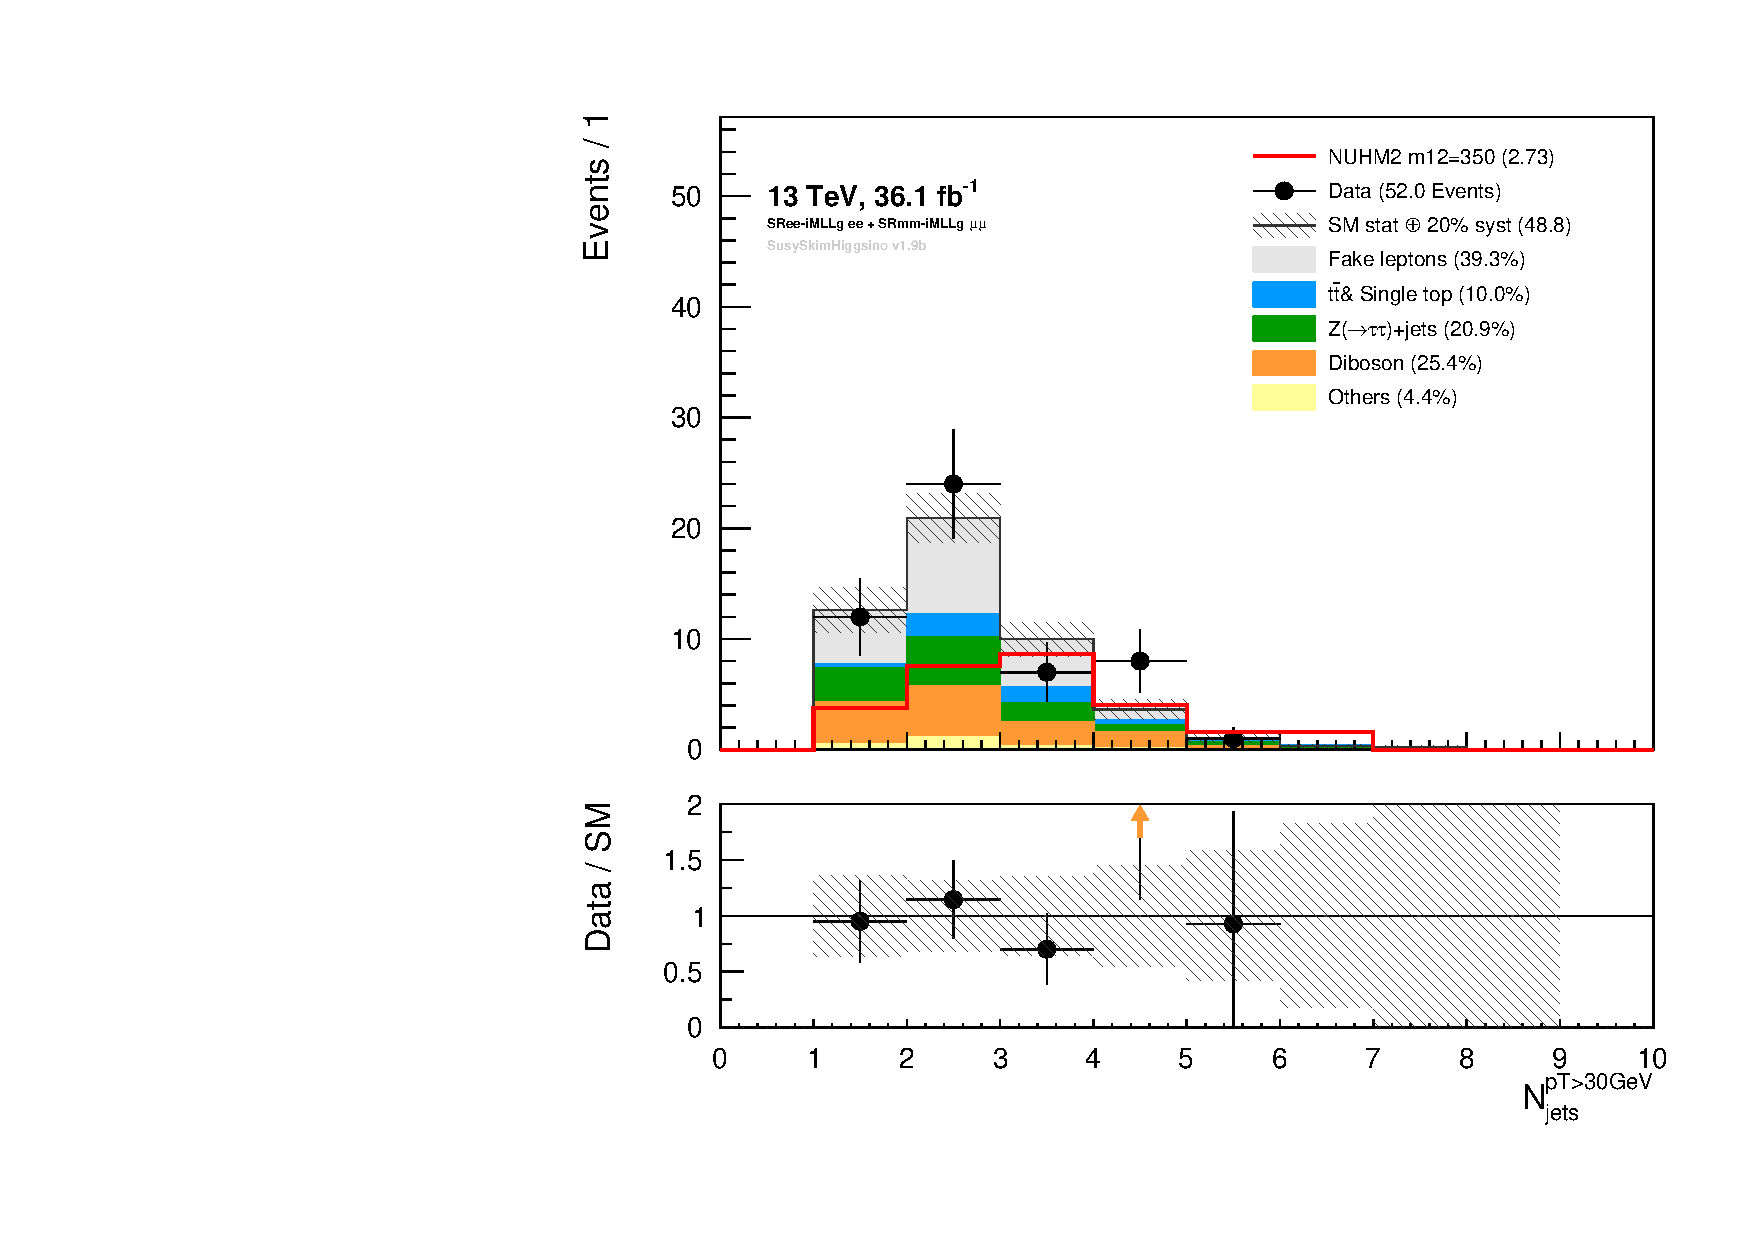
\includegraphics[scale=0.3]{NUHM2_m12_350_and_Bkg_nJet30_SFOS_N_minus_one_distribution_in_SR_times_10_on_Nsig.pdf}
            \caption{$N^{30}_{\mathrm{jets}}$}
            \label{fig:event_nuhm2_m12_350_nJet30_SFOS}
        \end{subfigure}
        \begin{subfigure}[b]{0.48\textwidth}
            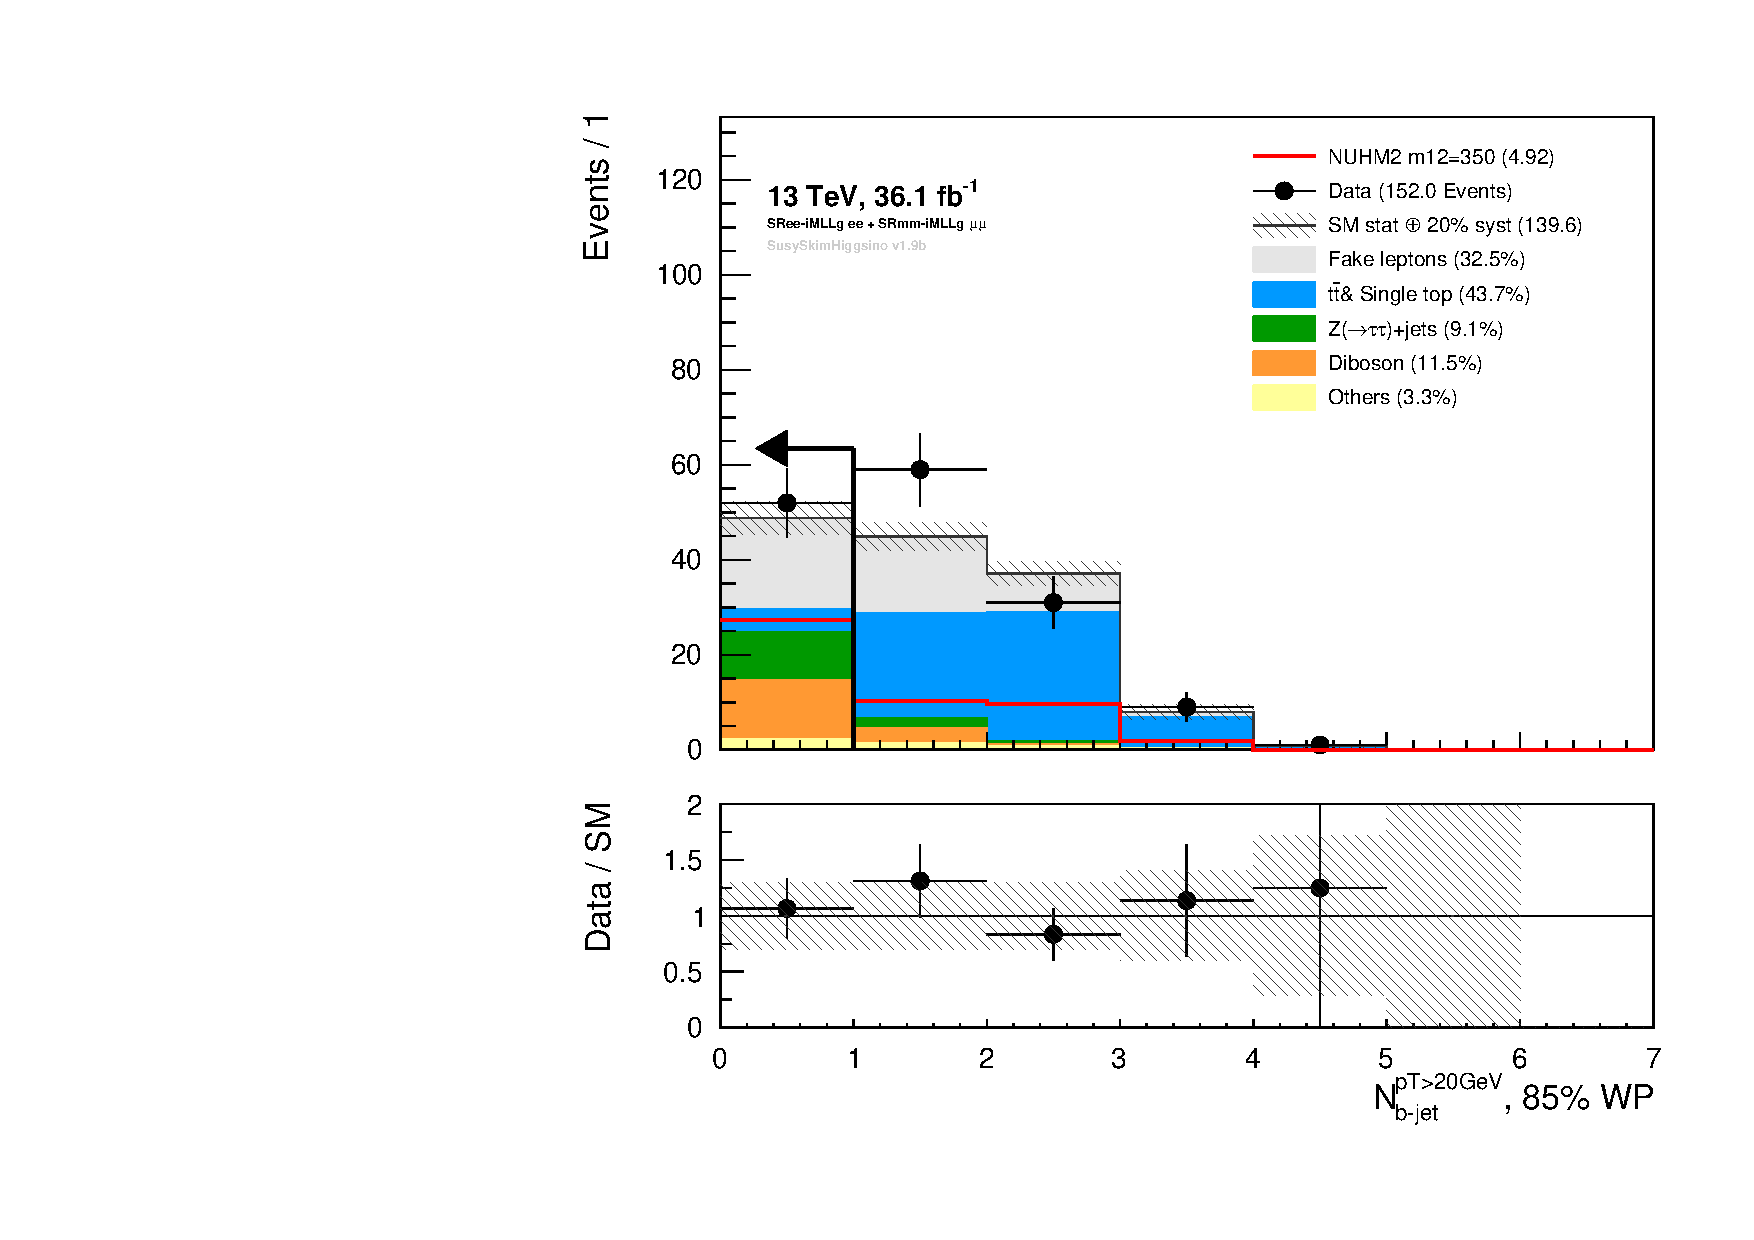
\includegraphics[scale=0.3]{NUHM2_m12_350_and_Bkg_nBJet20_MV2c10_SFOS_N_minus_one_distribution_in_SR_times_10_on_Nsig.pdf}
            \caption{$N^{20}_{\mathrm{b-jets}}$}
            \label{fig:event_nuhm2_m12_350_nBJet20_SFOS}
        \end{subfigure}
        \begin{subfigure}[b]{0.48\textwidth}
            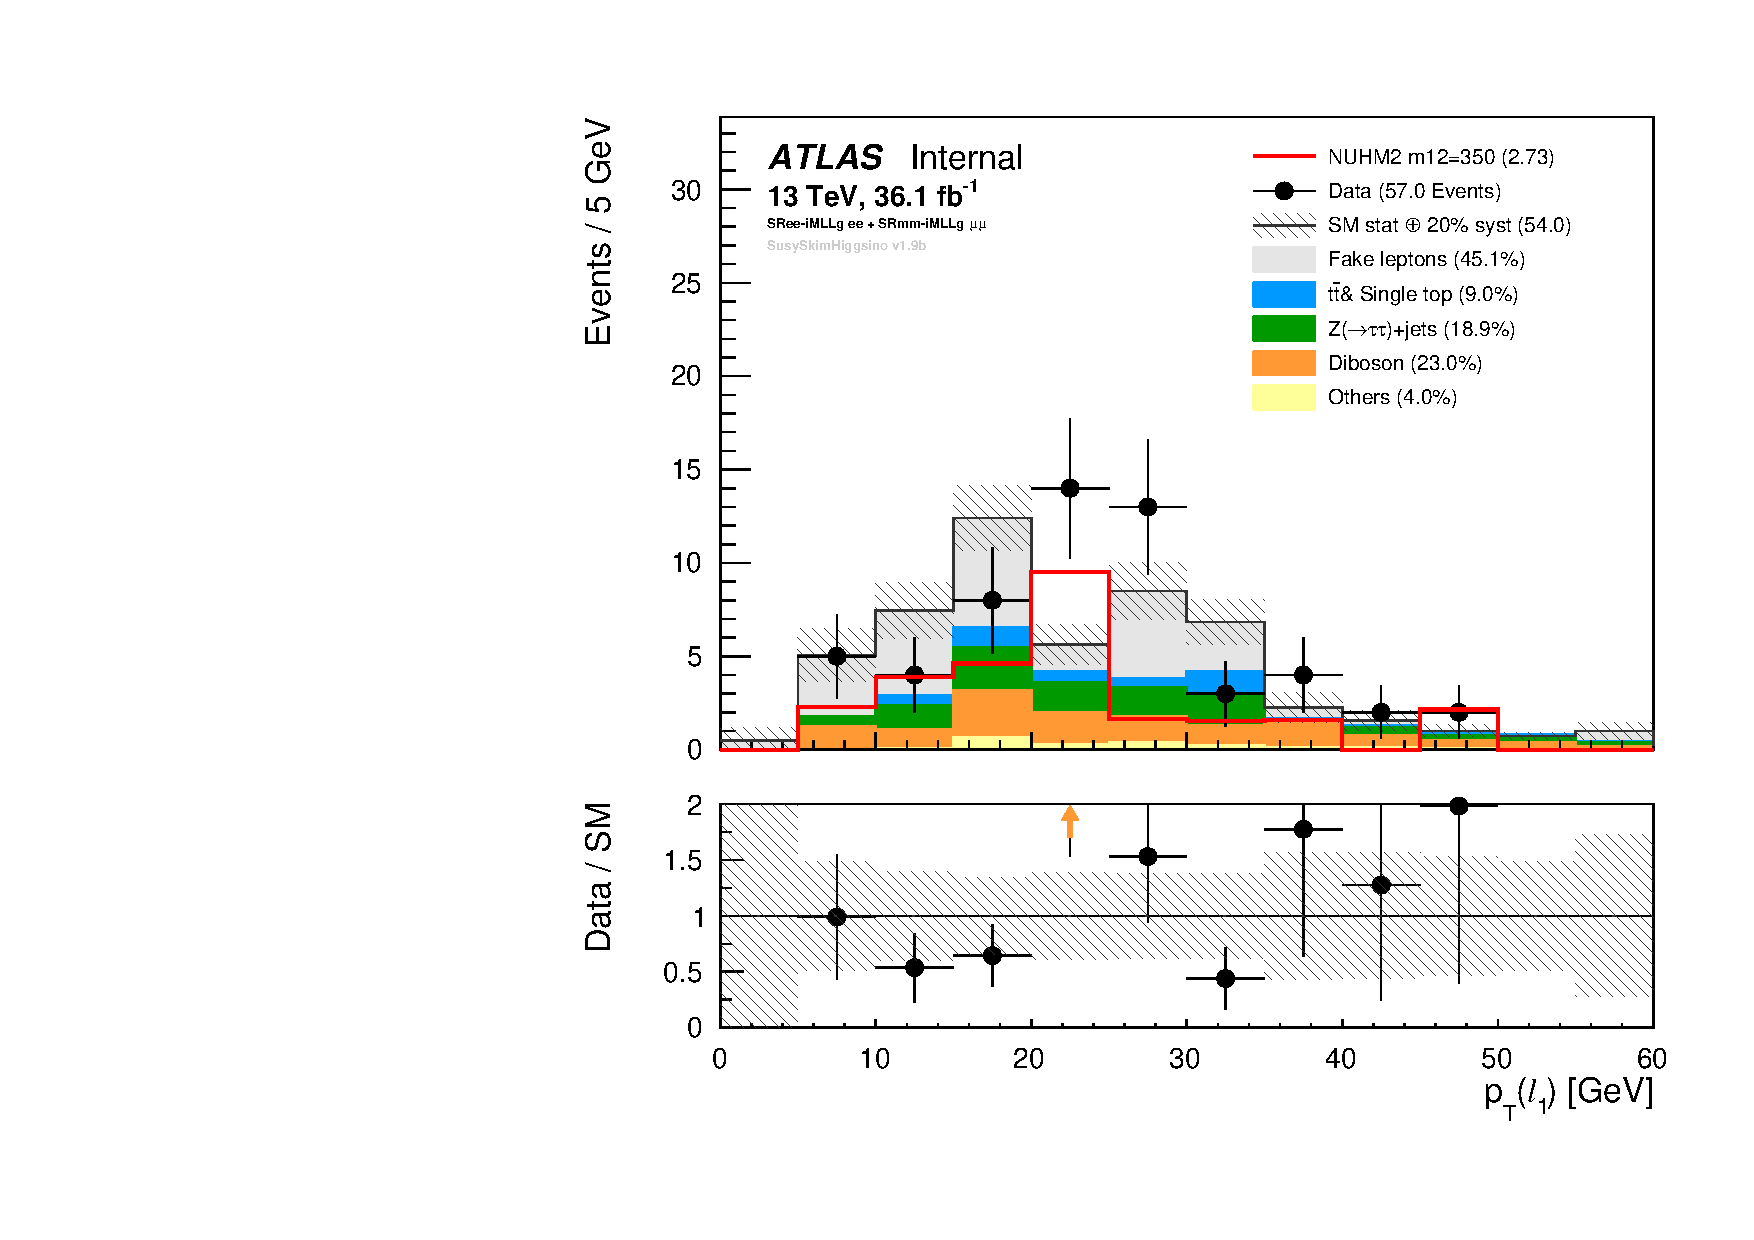
\includegraphics[scale=0.3]{NUHM2_m12_350_and_Bkg_lep1Pt_SFOS_N_minus_one_distribution_in_SR_times_10_on_Nsig.pdf}
            \caption{$p^{\ell_1}_{\mathrm{T}}$}
            \label{fig:event_nuhm2_m12_350_lep1Pt_SFOS}
        \end{subfigure}
        \begin{subfigure}[b]{0.48\textwidth}
            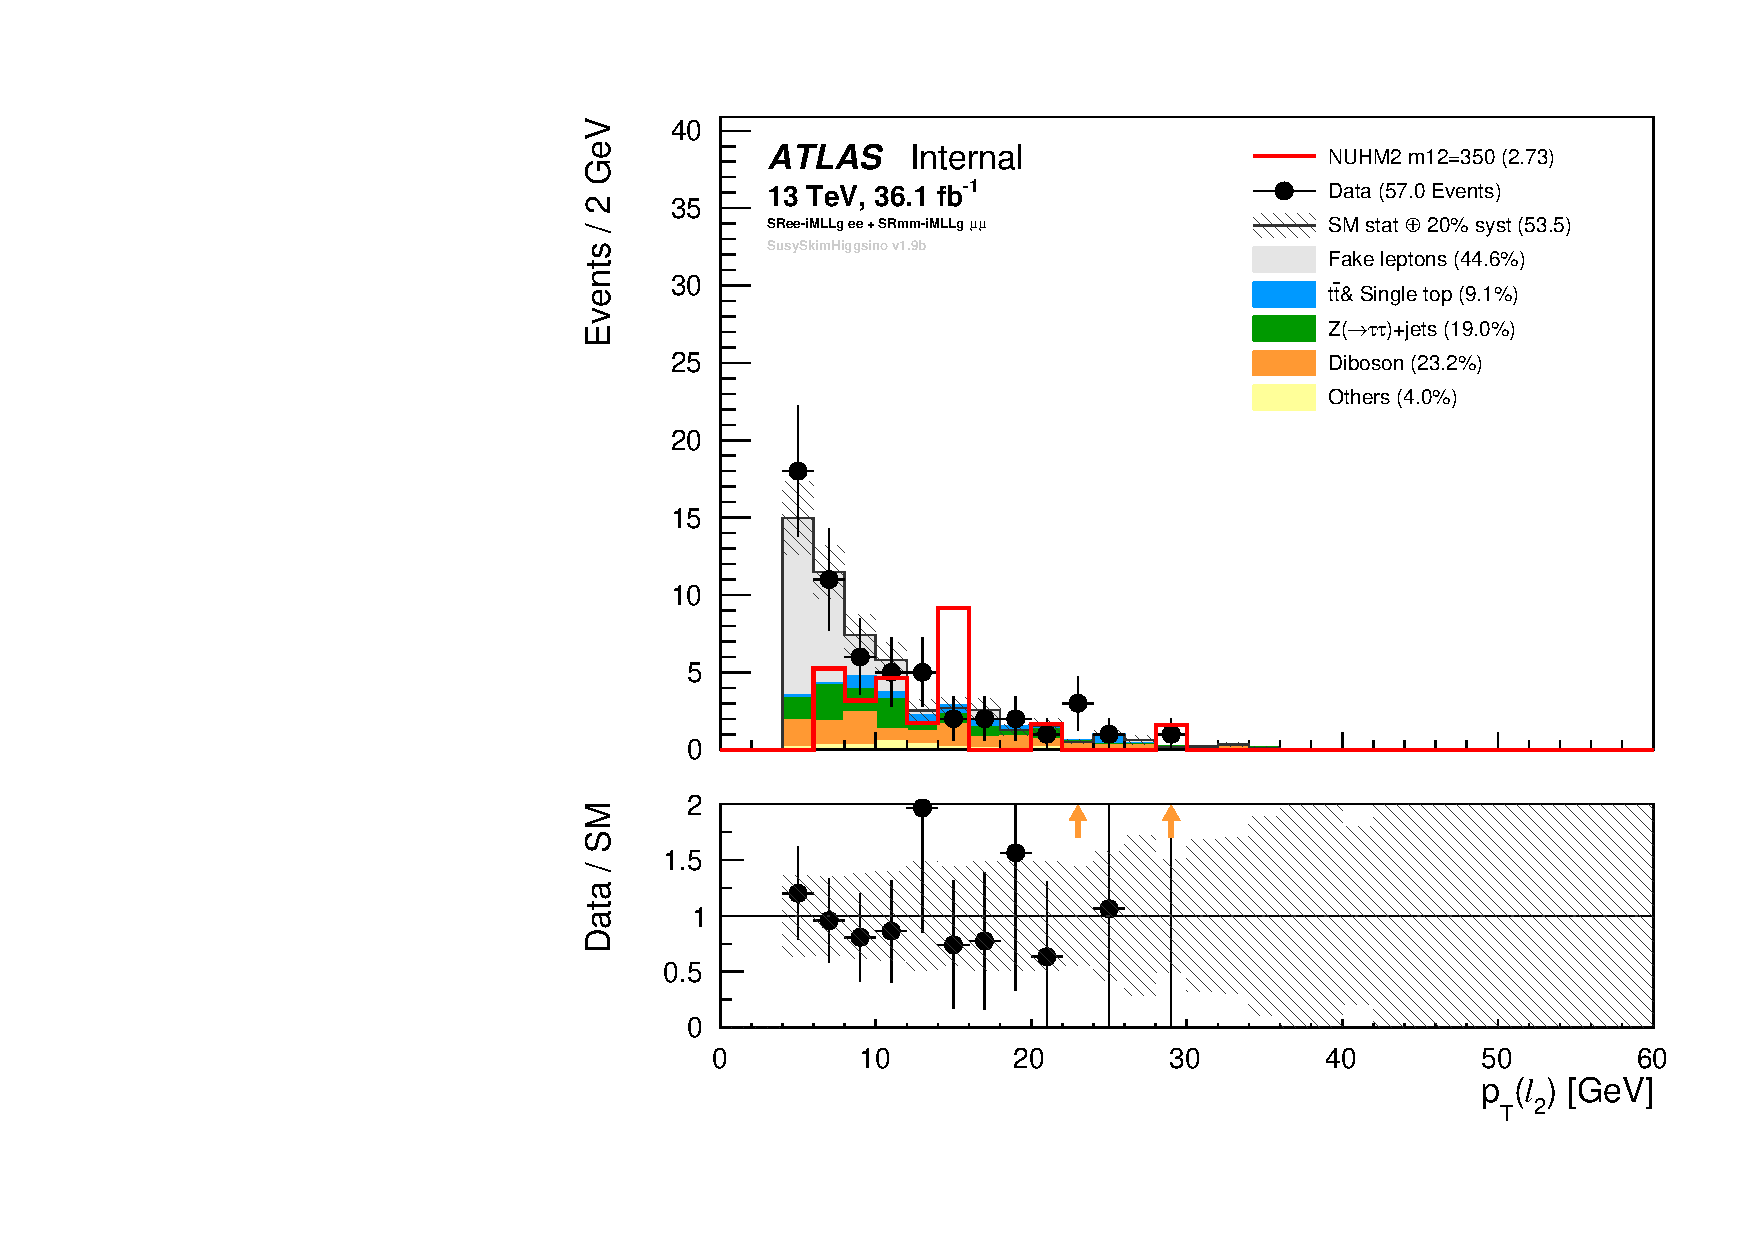
\includegraphics[scale=0.3]{NUHM2_m12_350_and_Bkg_lep2Pt_SFOS_N_minus_one_distribution_in_SR_times_10_on_Nsig.pdf}
            \caption{$p^{\ell_2}_{\mathrm{T}}$}
            \label{fig:event_nuhm2_m12_350_lep2Pt_SFOS}
        \end{subfigure}
        \begin{subfigure}[b]{0.48\textwidth}
            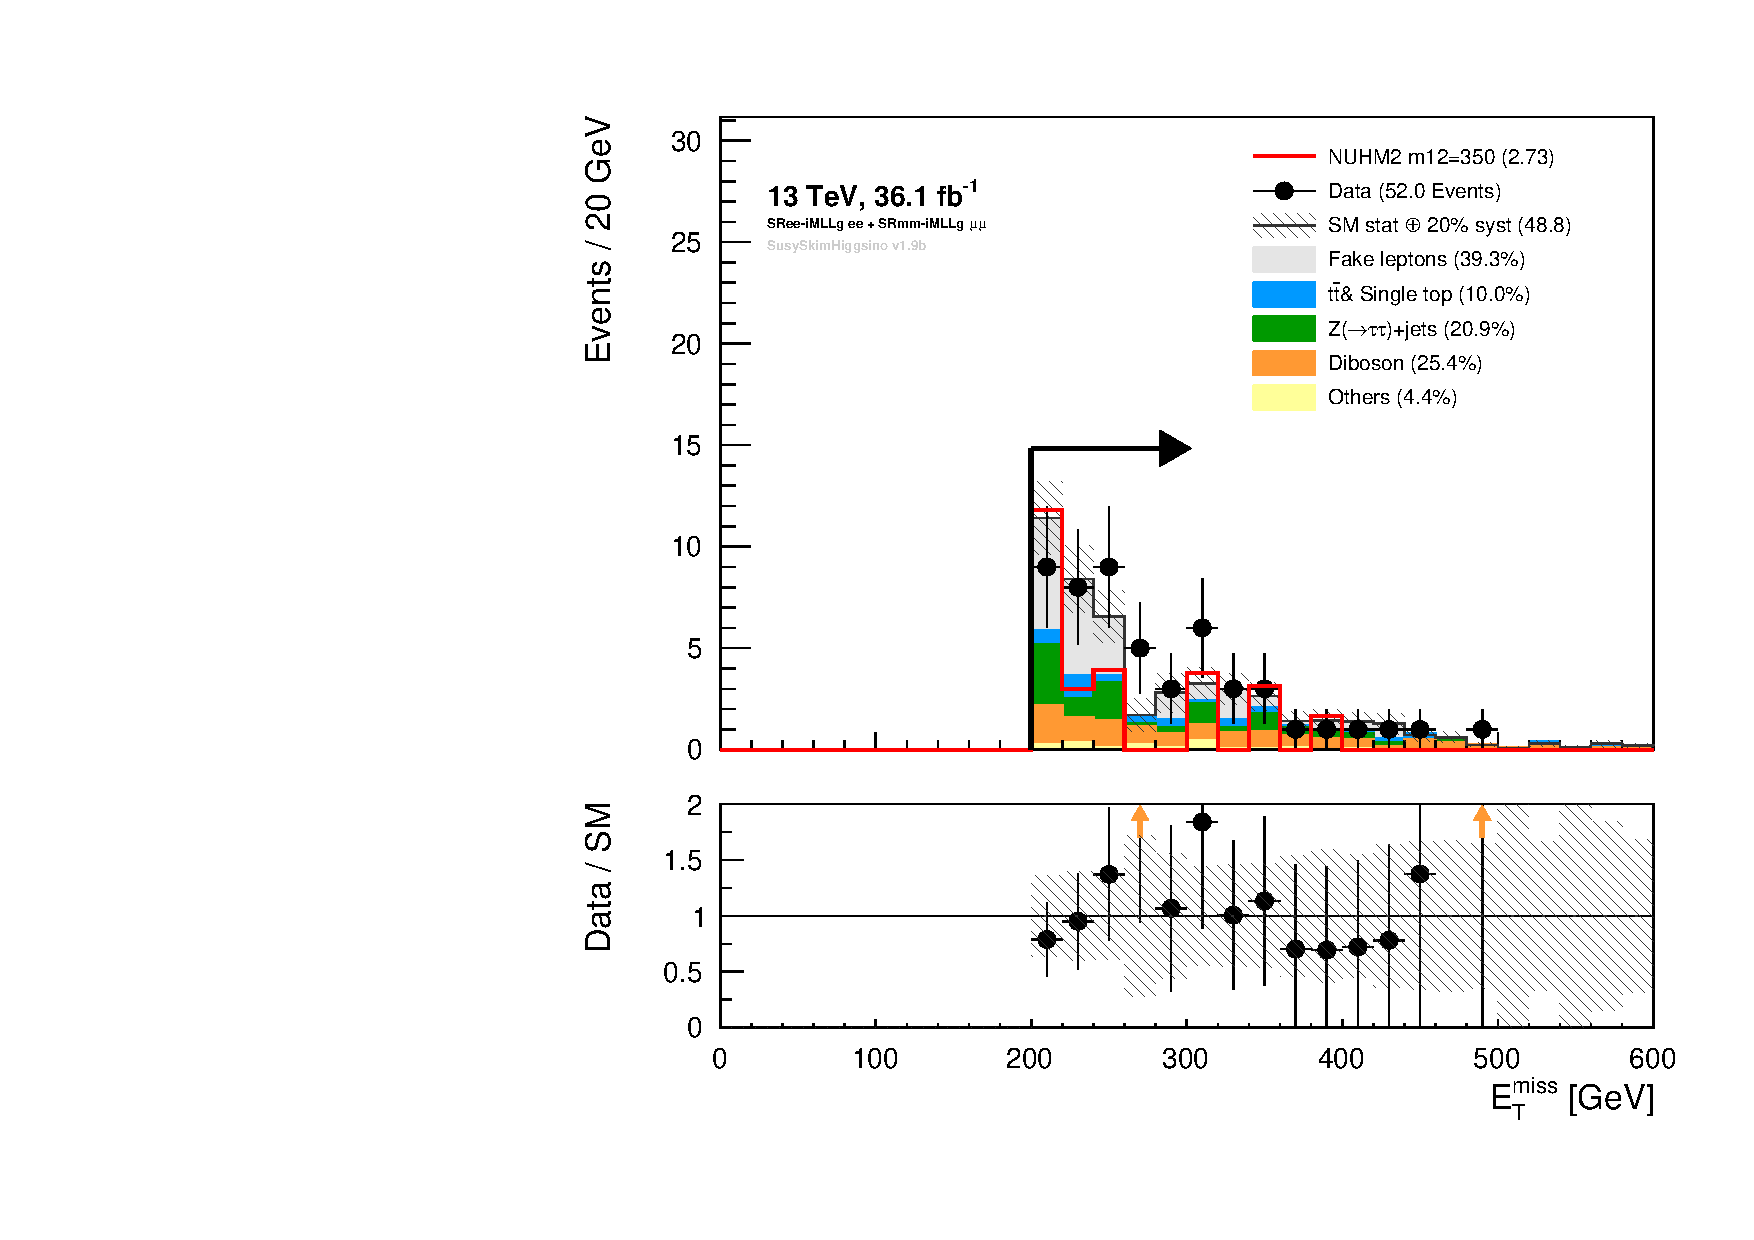
\includegraphics[scale=0.3]{NUHM2_m12_350_and_Bkg_met_Et_SFOS_N_minus_one_distribution_in_SR_times_10_on_Nsig.pdf}
            \caption{$E^{\mathrm{miss}}_{\mathrm{T}}$}
            \label{fig:event_nuhm2_m12_350_met_SFOS}
        \end{subfigure}
        \begin{subfigure}[b]{0.48\textwidth}
            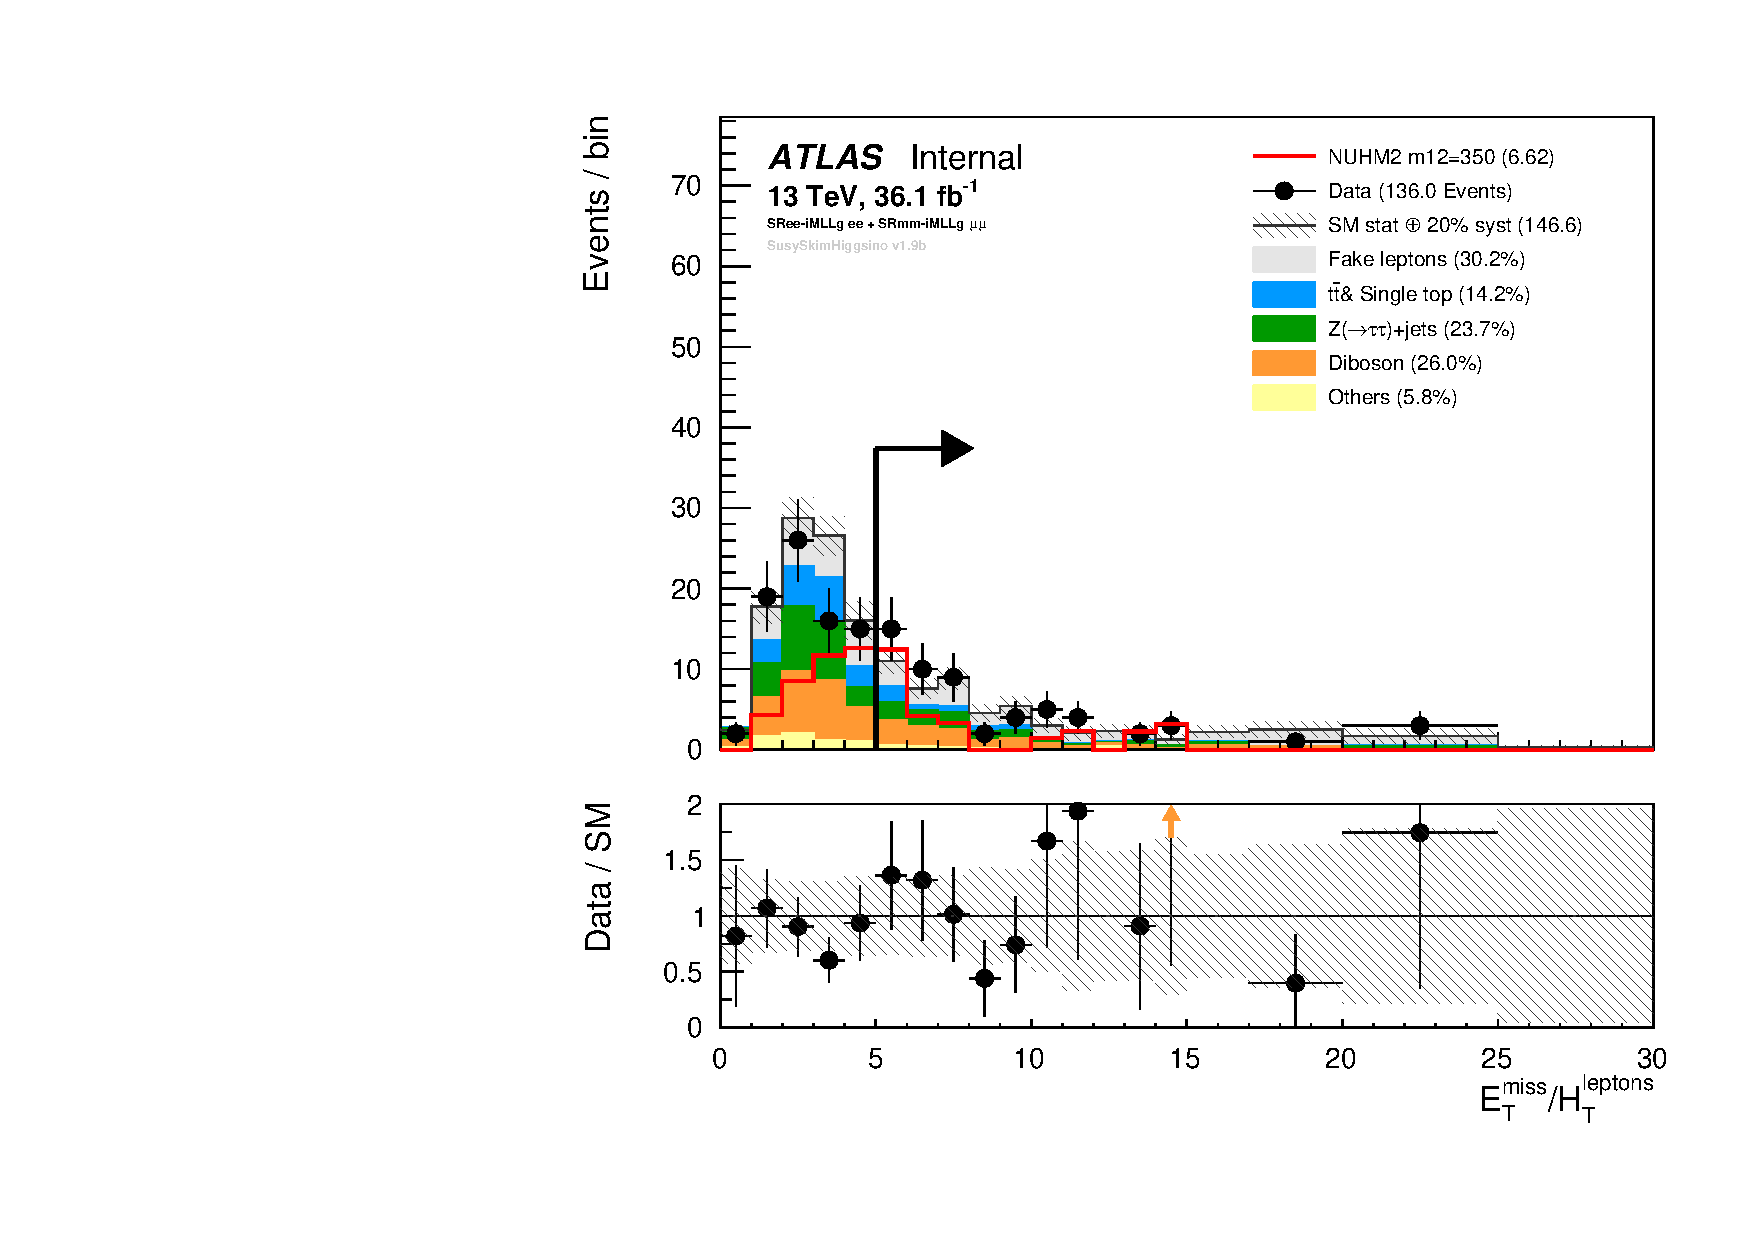
\includegraphics[scale=0.3]{NUHM2_m12_350_and_Bkg_METOverHTLep_SFOS_N_minus_one_distribution_in_SR_times_10_on_Nsig.pdf}
            \caption{$E^{\mathrm{miss}}_{\mathrm{T}} / H^{\mathrm{leptons}}_{\mathrm{T}}$}
            \label{fig:event_nuhm2_m12_350_METOverHTLep_SFOS}
        \end{subfigure}
    \end{center}
    \caption{The `$N-1$' distributions for NUHM2 model with $m_{1/2} = 350$~{\GeV} in SR region $1 < $SR$\ell \ell$-$m_{\ell \ell} < 60$~{\GeV}.
    The NUHM2 distributions are multiplied by 10 but the number of events in the legend use its actual values.}
    \label{fig:event_nuhm2_kinematic_in_SR_SFOS_m12_350_1}
\end{figure}

\begin{figure}[htbp]
    \begin{center}
        \begin{subfigure}[b]{0.48\textwidth}
            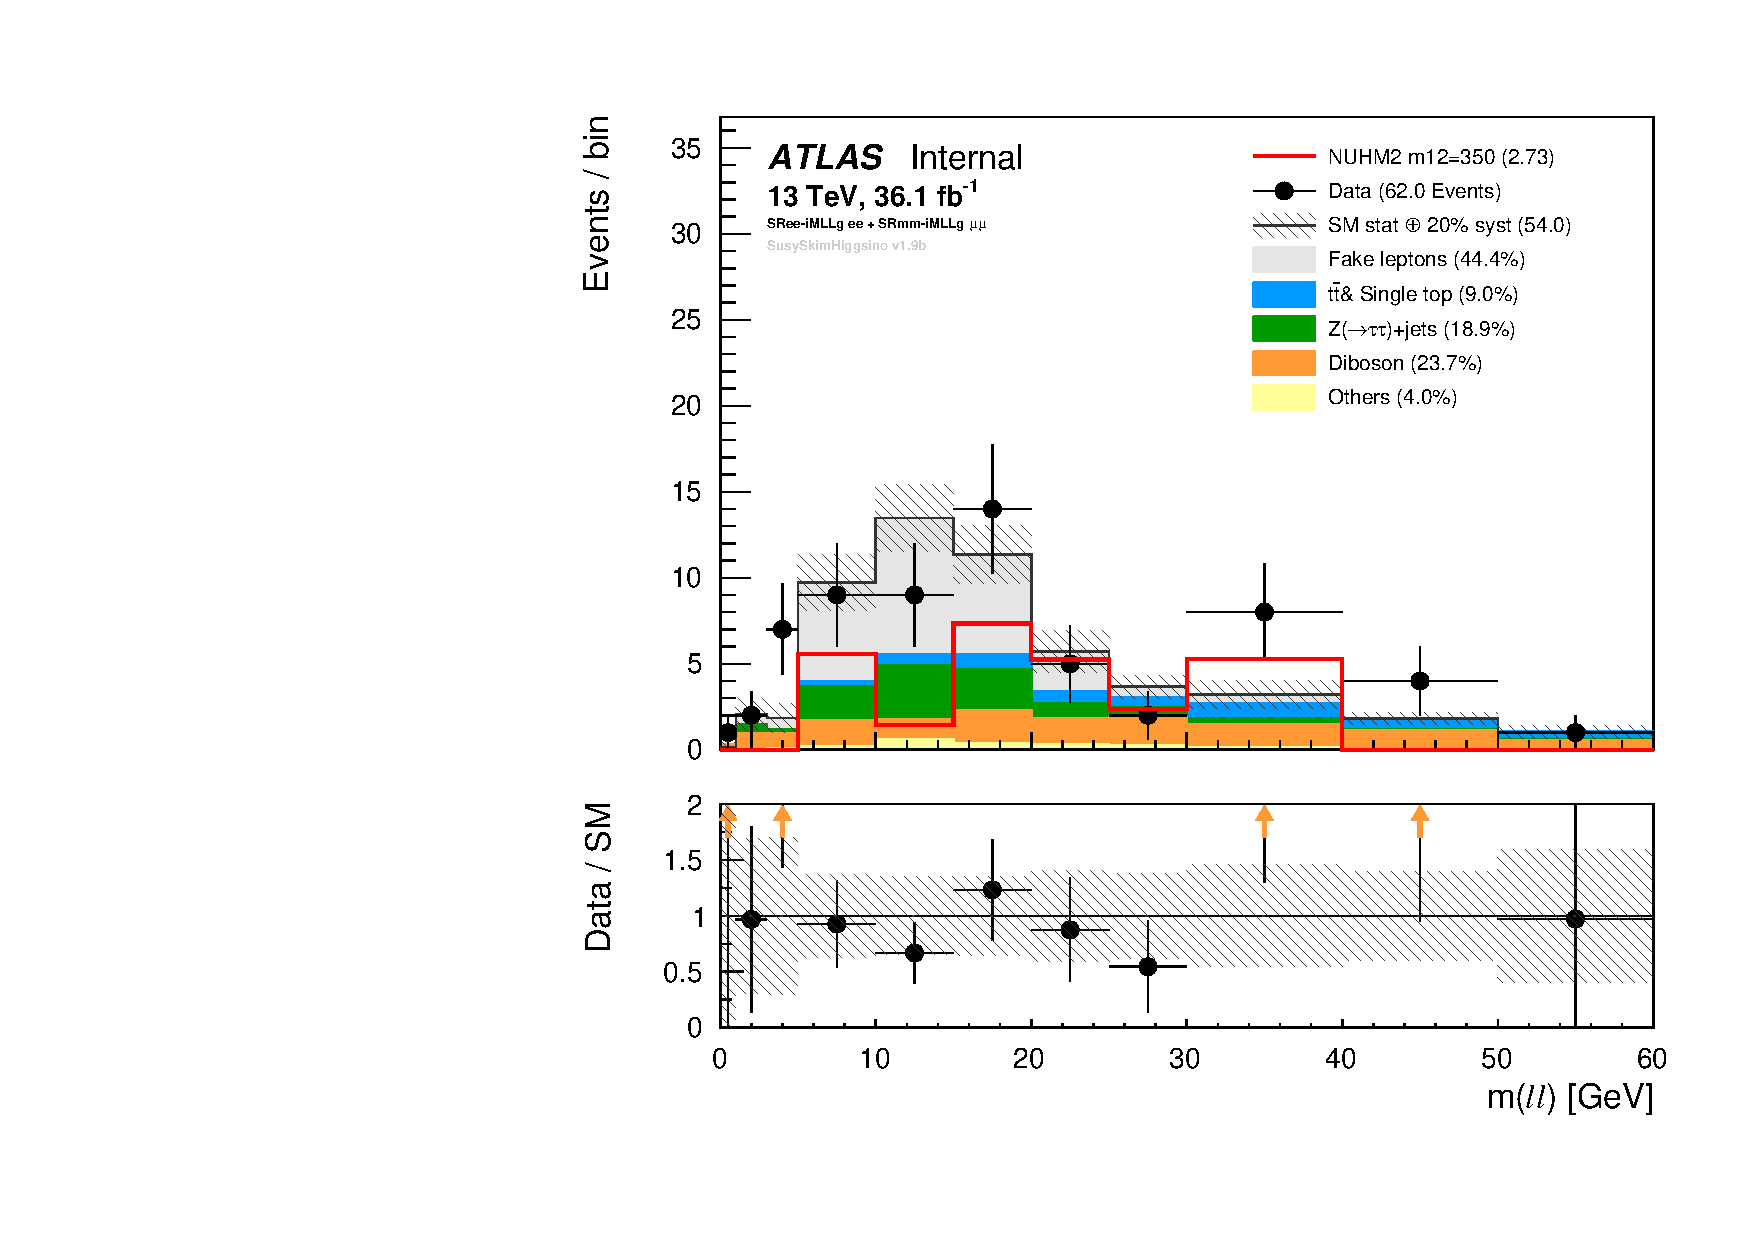
\includegraphics[scale=0.3]{NUHM2_m12_350_and_Bkg_mll_SFOS_N_minus_one_distribution_in_SR_times_10_on_Nsig.pdf}
            \caption{$m_{\ell\ell}$}
            \label{fig:event_nuhm2_m12_350_mll_SFOS}
        \end{subfigure}
        \begin{subfigure}[b]{0.48\textwidth}
            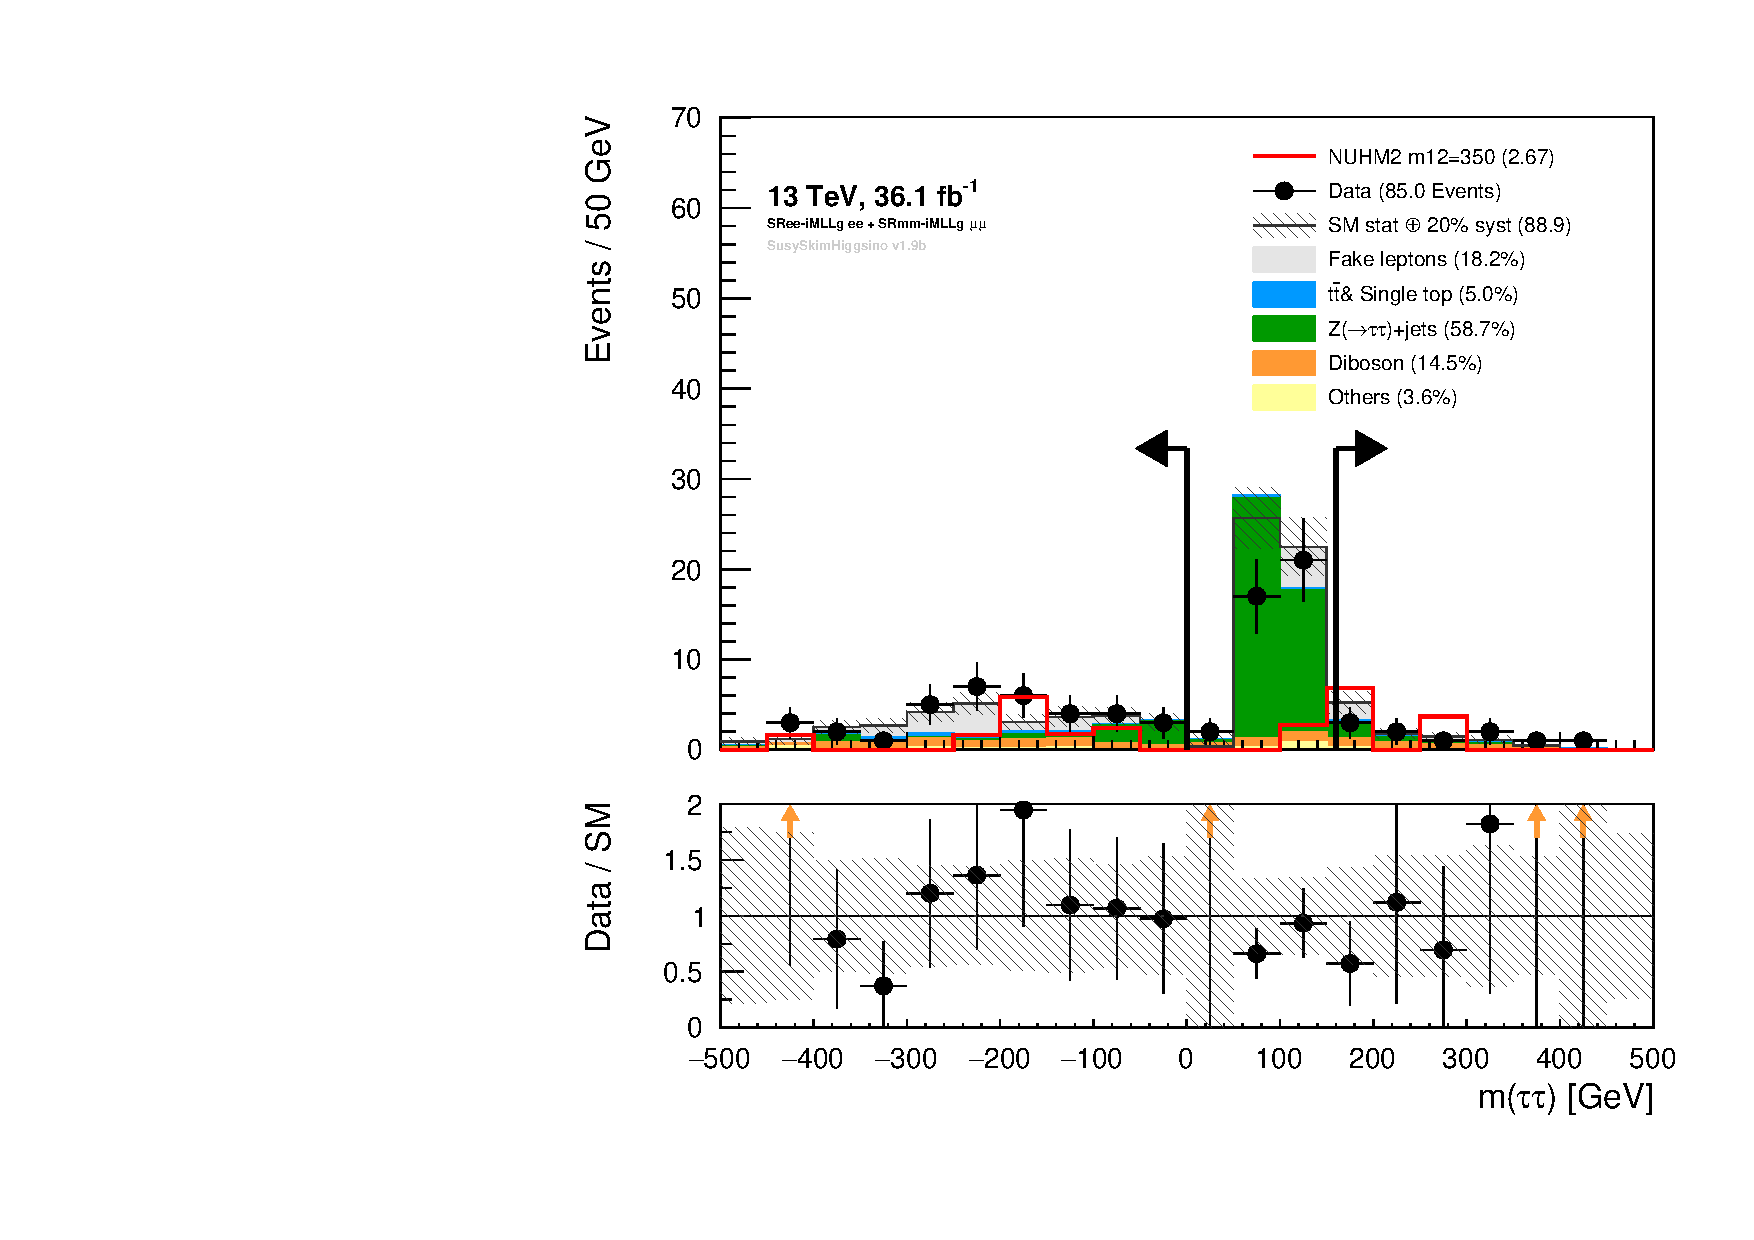
\includegraphics[scale=0.3]{NUHM2_m12_350_and_Bkg_MTauTau_SFOS_N_minus_one_distribution_in_SR_times_10_on_Nsig.pdf}
            \caption{$m_{\tau\tau}$}
            \label{fig:event_nuhm2_m12_350_MTauTau_SFOS}
        \end{subfigure}
        \begin{subfigure}[b]{0.48\textwidth}
            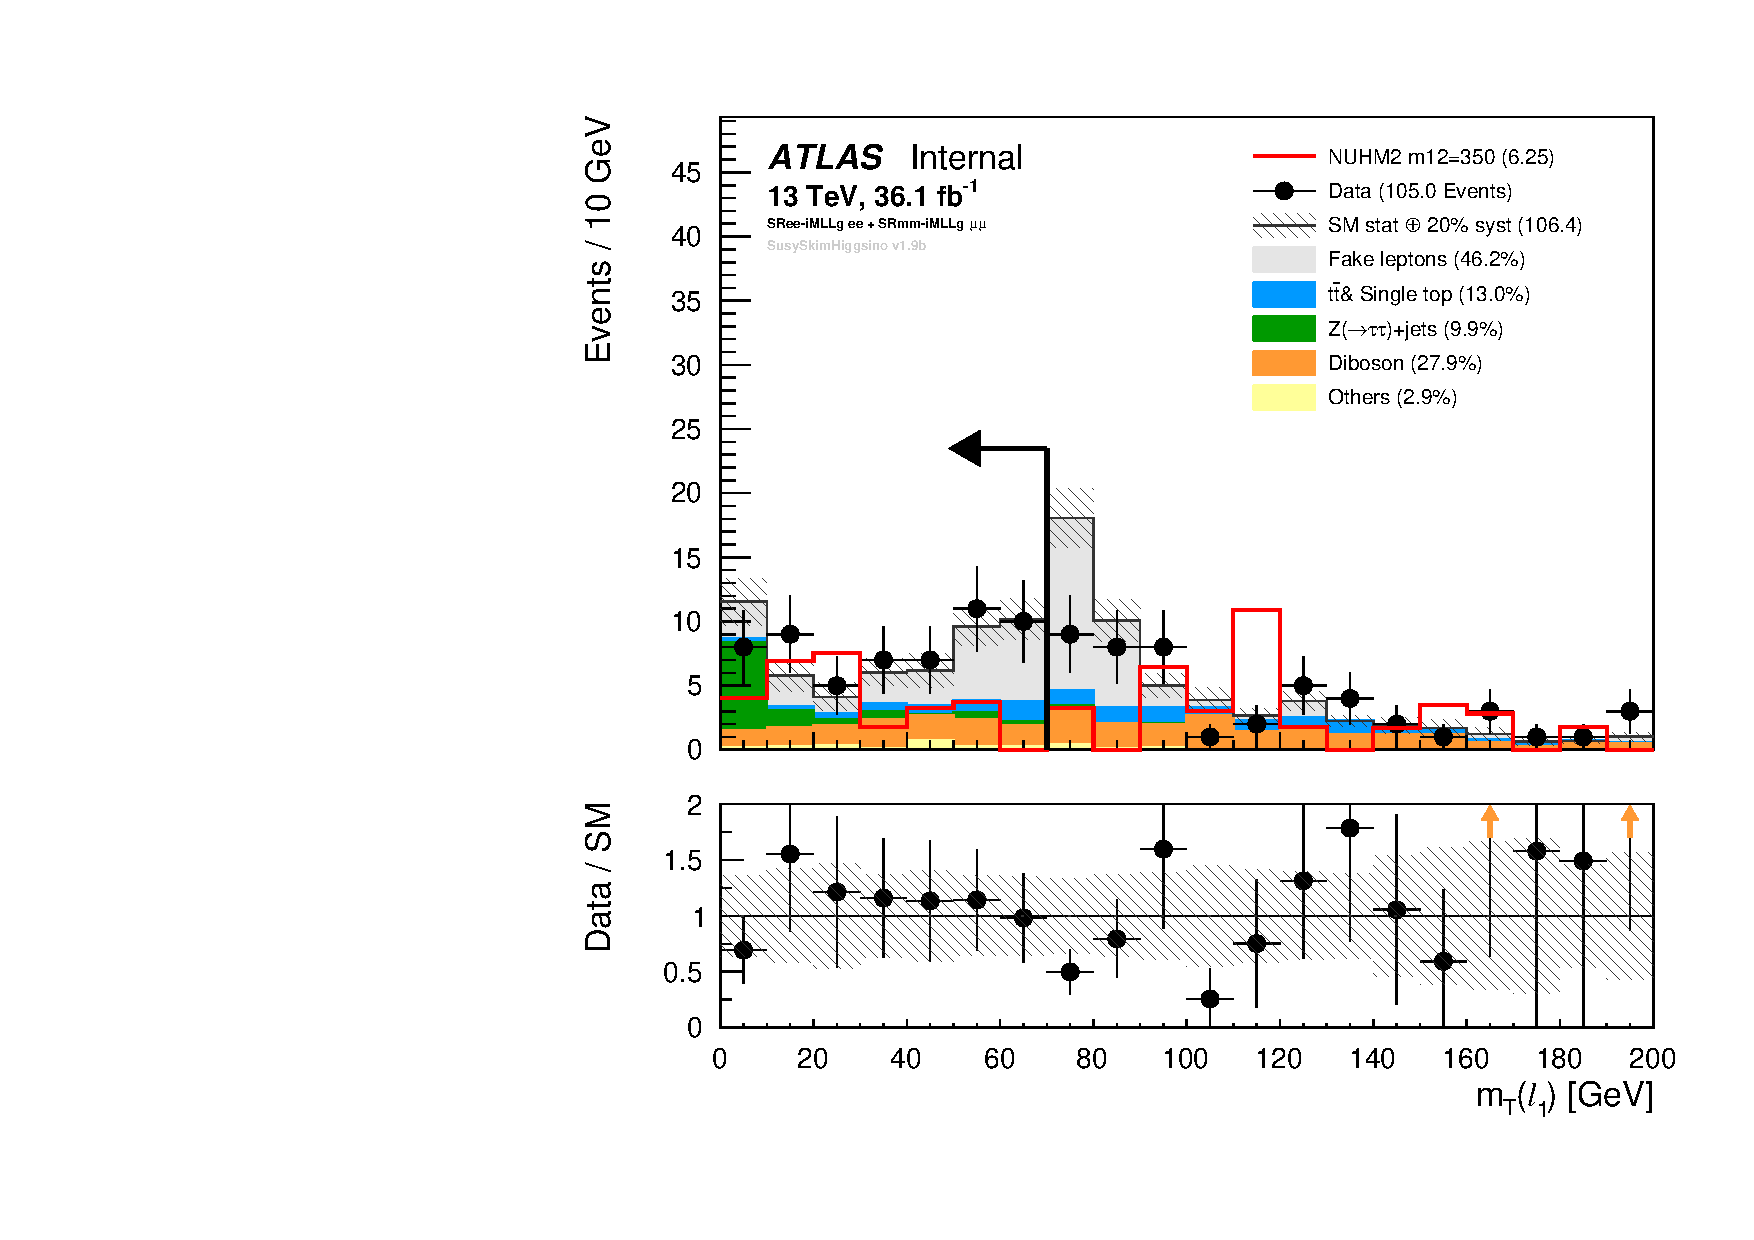
\includegraphics[scale=0.3]{NUHM2_m12_350_and_Bkg_mt_lep1_SFOS_N_minus_one_distribution_in_SR_times_10_on_Nsig.pdf}
            \caption{$m_{T}(\ell_{1})$}
            \label{fig:event_nuhm2_m12_350_mt_lep1_SFOS}
        \end{subfigure}
        \begin{subfigure}[b]{0.48\textwidth}
            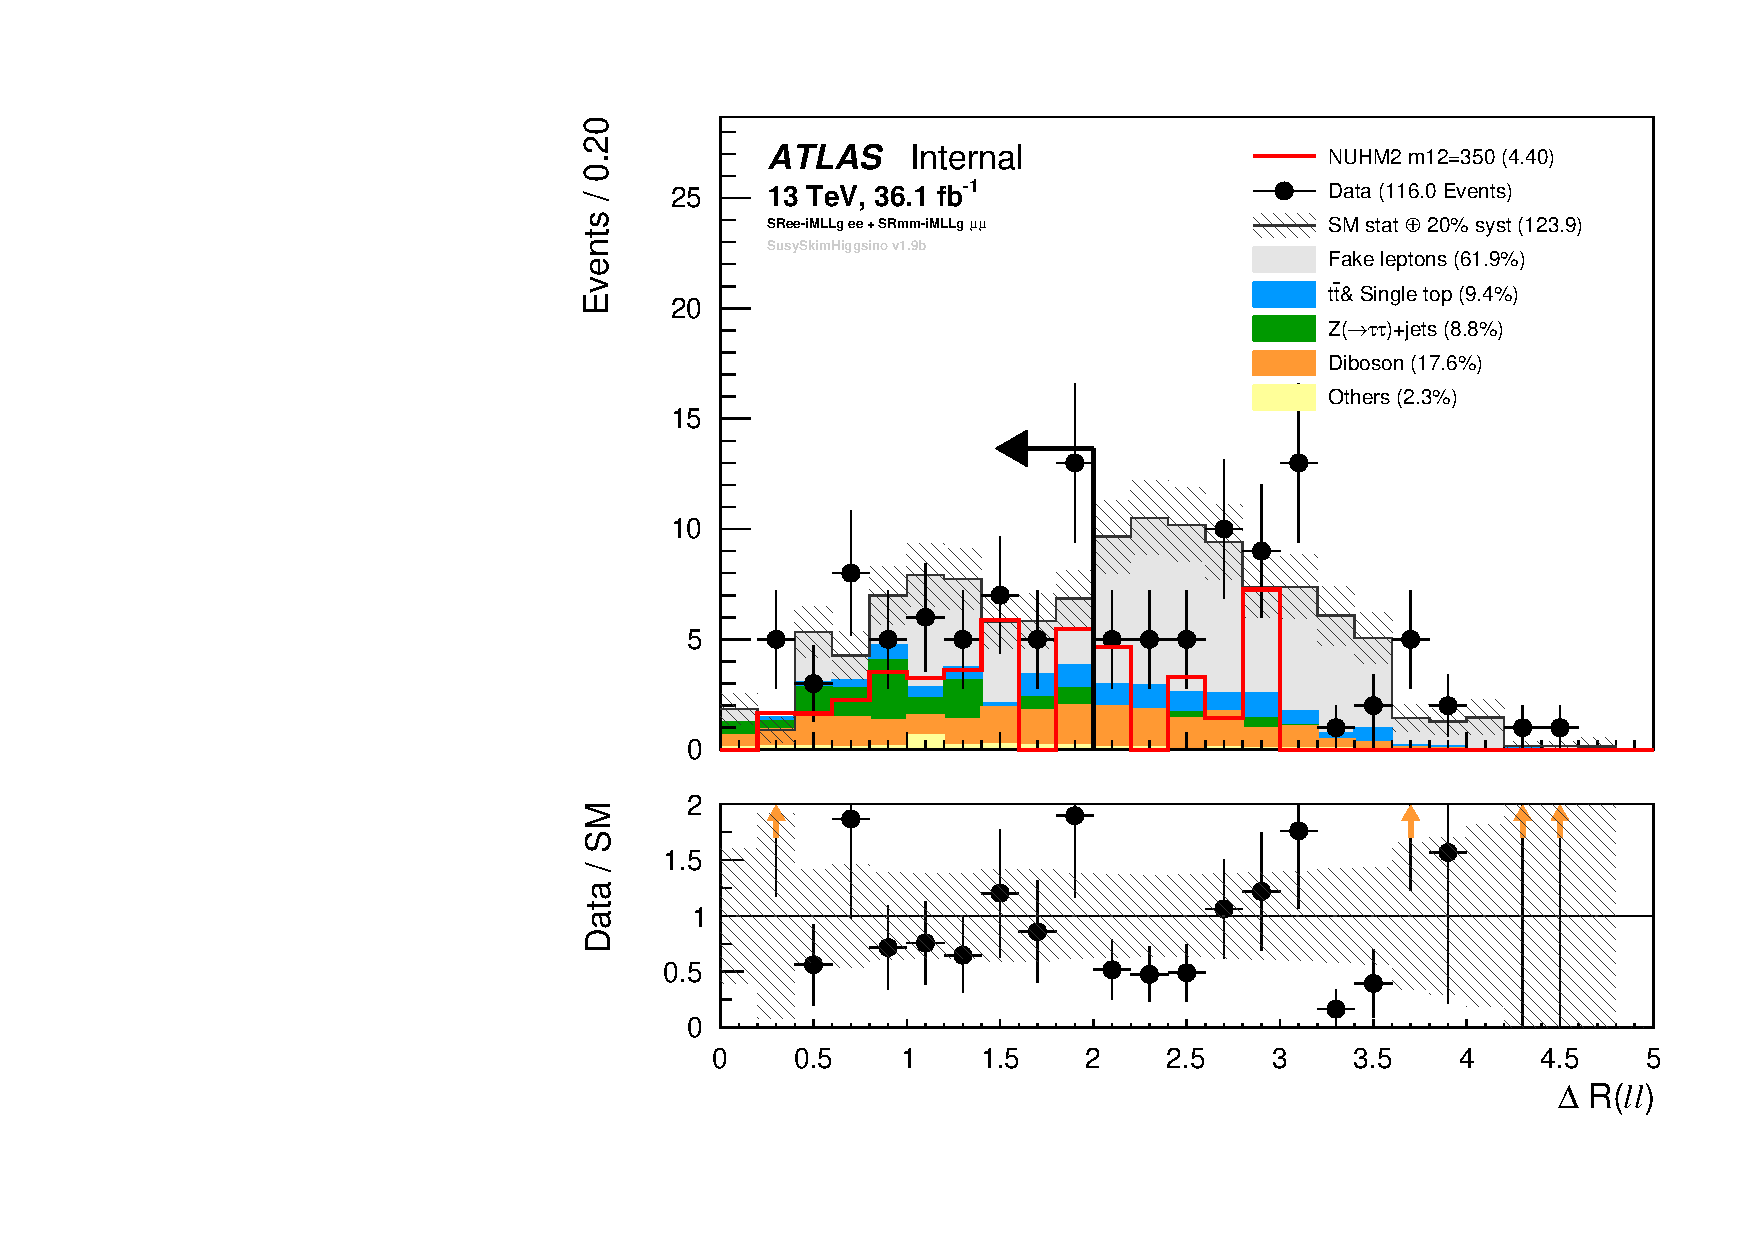
\includegraphics[scale=0.3]{NUHM2_m12_350_and_Bkg_Rll_SFOS_N_minus_one_distribution_in_SR_times_10_on_Nsig.pdf}
            \caption{$\Delta R_{\ell\ell}$}
            \label{fig:event_nuhm2_m12_350_Rll_SFOS}
        \end{subfigure}
        \begin{subfigure}[b]{0.48\textwidth}
            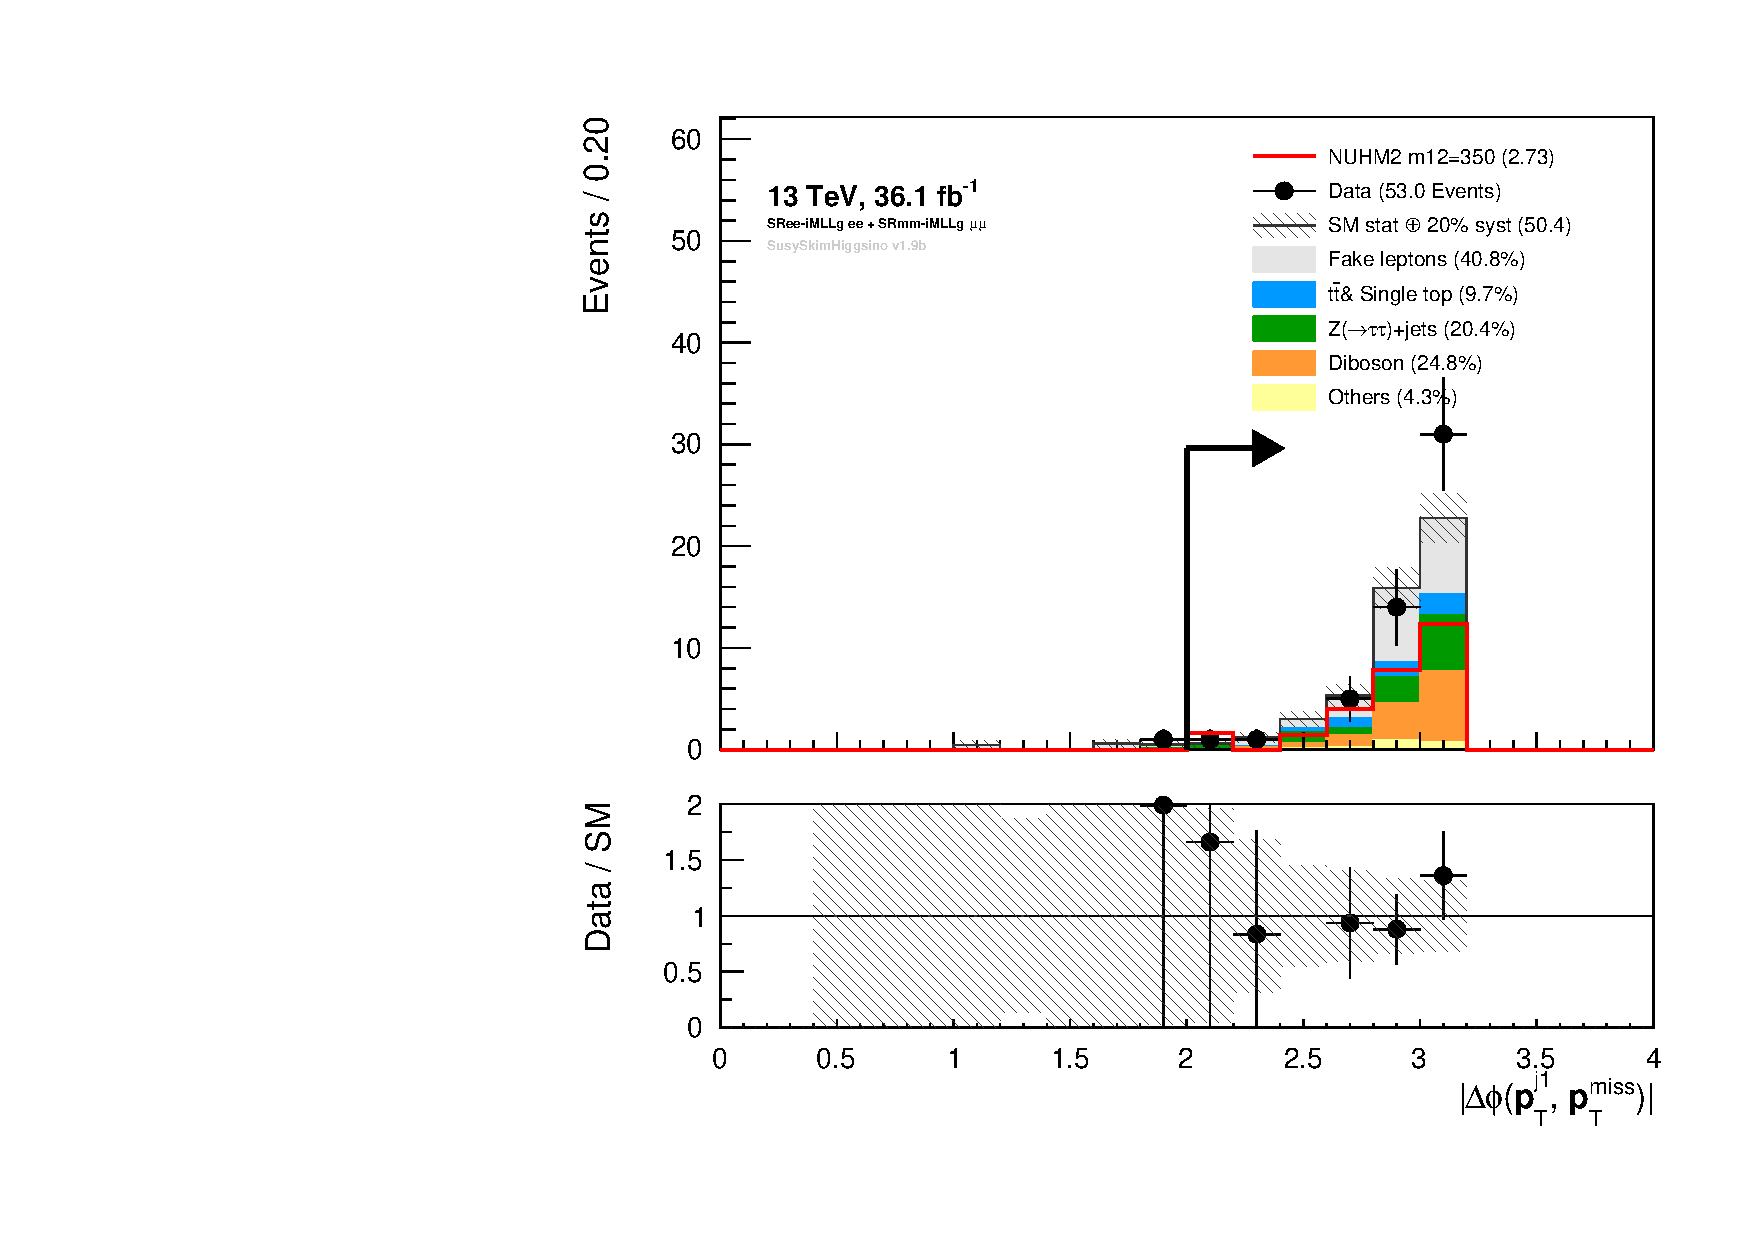
\includegraphics[scale=0.3]{NUHM2_m12_350_and_Bkg_DPhiJ1Met_SFOS_N_minus_one_distribution_in_SR_times_10_on_Nsig.pdf}
            \caption{$|\Delta \phi(\mathbf{p}^{j_{1}}_{\mathrm{T}}, \mathbf{p}^{\mathrm{miss}}_{\mathrm{T}})|$}
            \label{fig:event_nuhm2_m12_350_DPhiJ1Met_SFOS}
        \end{subfigure}
        \begin{subfigure}[b]{0.48\textwidth}
            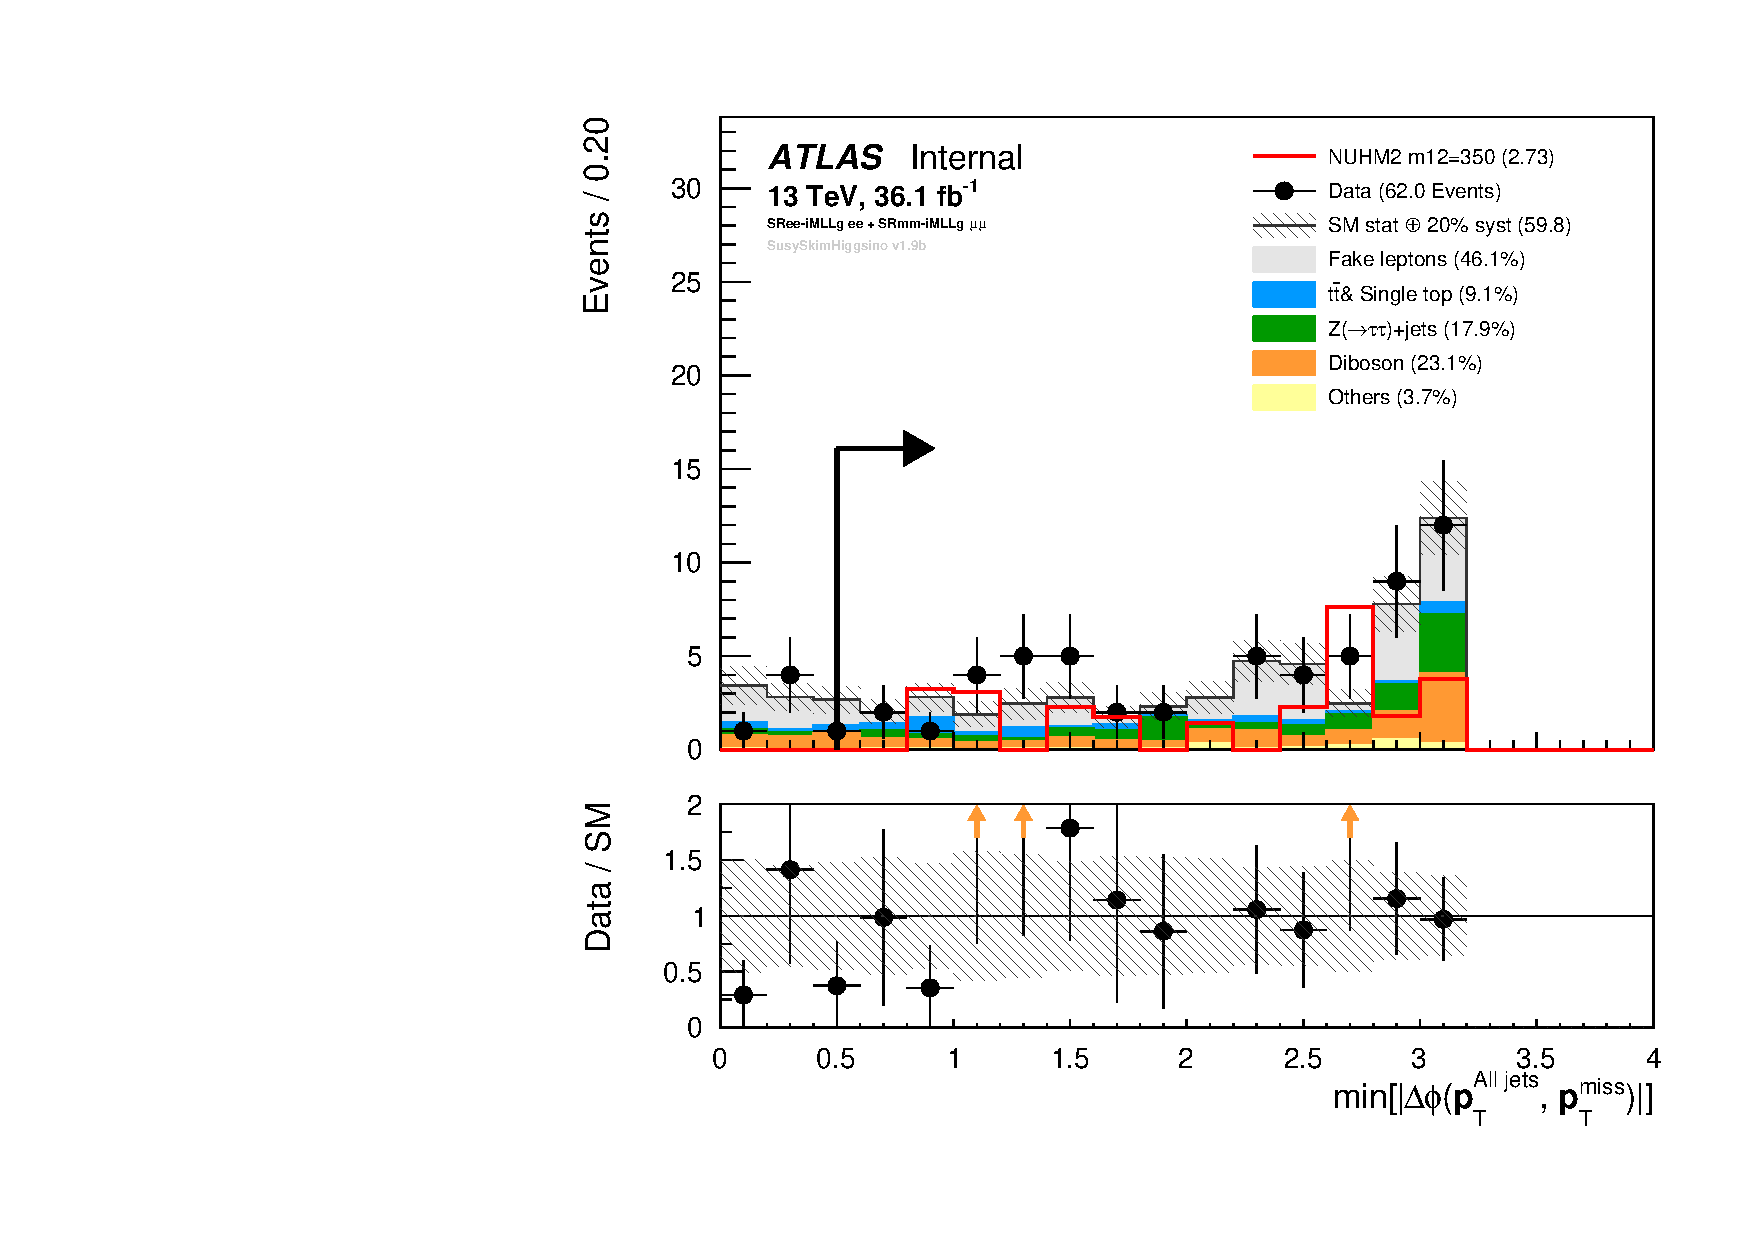
\includegraphics[scale=0.3]{NUHM2_m12_350_and_Bkg_minDPhiAllJetsMet_SFOS_N_minus_one_distribution_in_SR_times_10_on_Nsig.pdf}
            \caption{min[$|\Delta \phi(\mathbf{p}^{\textrm{All jets}}_{\mathrm{T}}, \mathbf{p}^{\mathrm{miss}}_{\mathrm{T}})|$]}
            \label{fig:event_nuhm2_m12_350_minDPhiAllJetsMet_SFOS}
        \end{subfigure}
    \end{center}
    \caption{The `$N-1$' distributions for NUHM2 model with $m_{1/2} = 350$~{\GeV} in SR region $1 < $SR$\ell \ell$-$m_{\ell \ell} < 60$~{\GeV}.
    The NUHM2 distributions are multiplied by 10 but the number of events in the legend use its actual values.}
    \label{fig:event_nuhm2_kinematic_in_SR_SFOS_m12_350_2}
\end{figure}

% m12 = 400
\begin{figure}[htbp]
    \begin{center}
        \begin{subfigure}[b]{0.48\textwidth}
            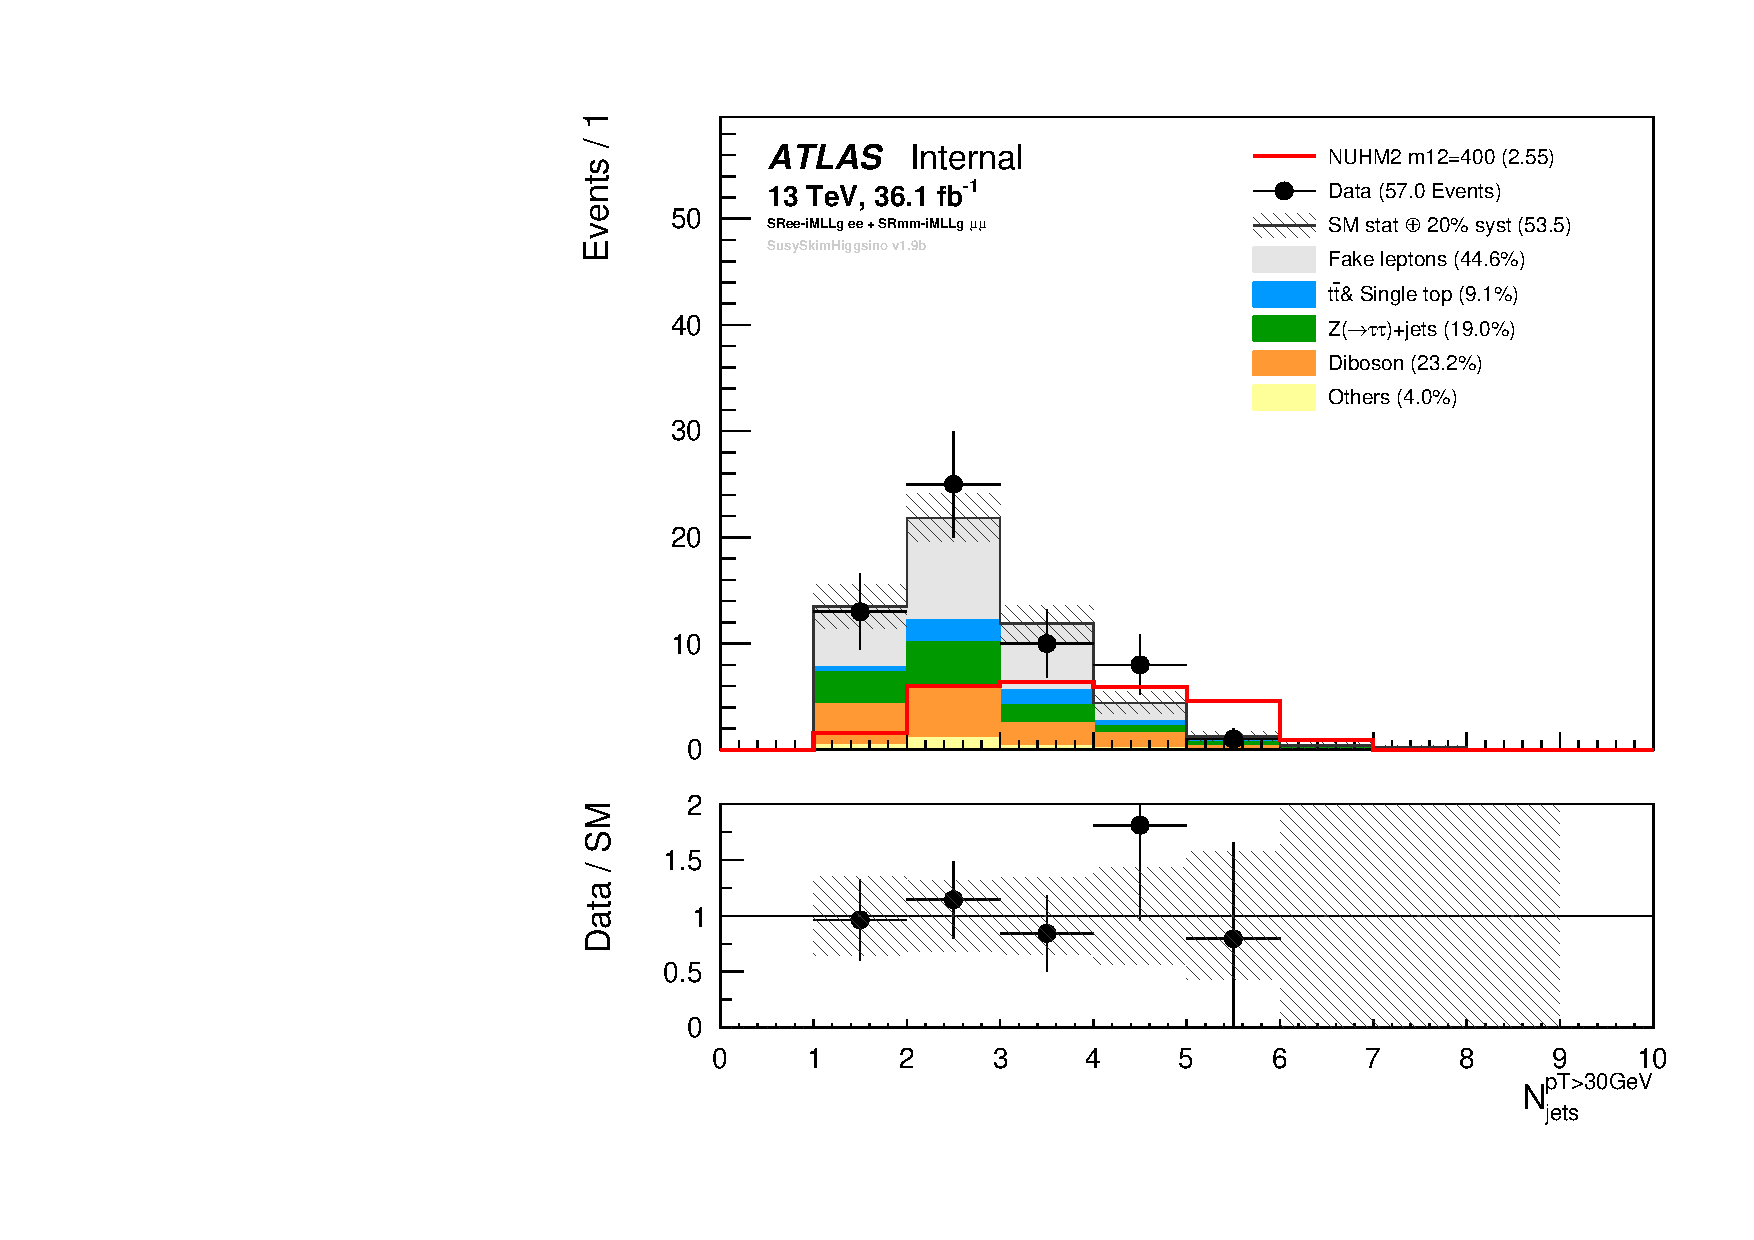
\includegraphics[scale=0.3]{NUHM2_m12_400_and_Bkg_nJet30_SFOS_N_minus_one_distribution_in_SR_times_10_on_Nsig.pdf}
            \caption{$N^{30}_{\mathrm{jets}}$}
            \label{fig:event_nuhm2_m12_400_nJet30_SFOS}
        \end{subfigure}
        \begin{subfigure}[b]{0.48\textwidth}
            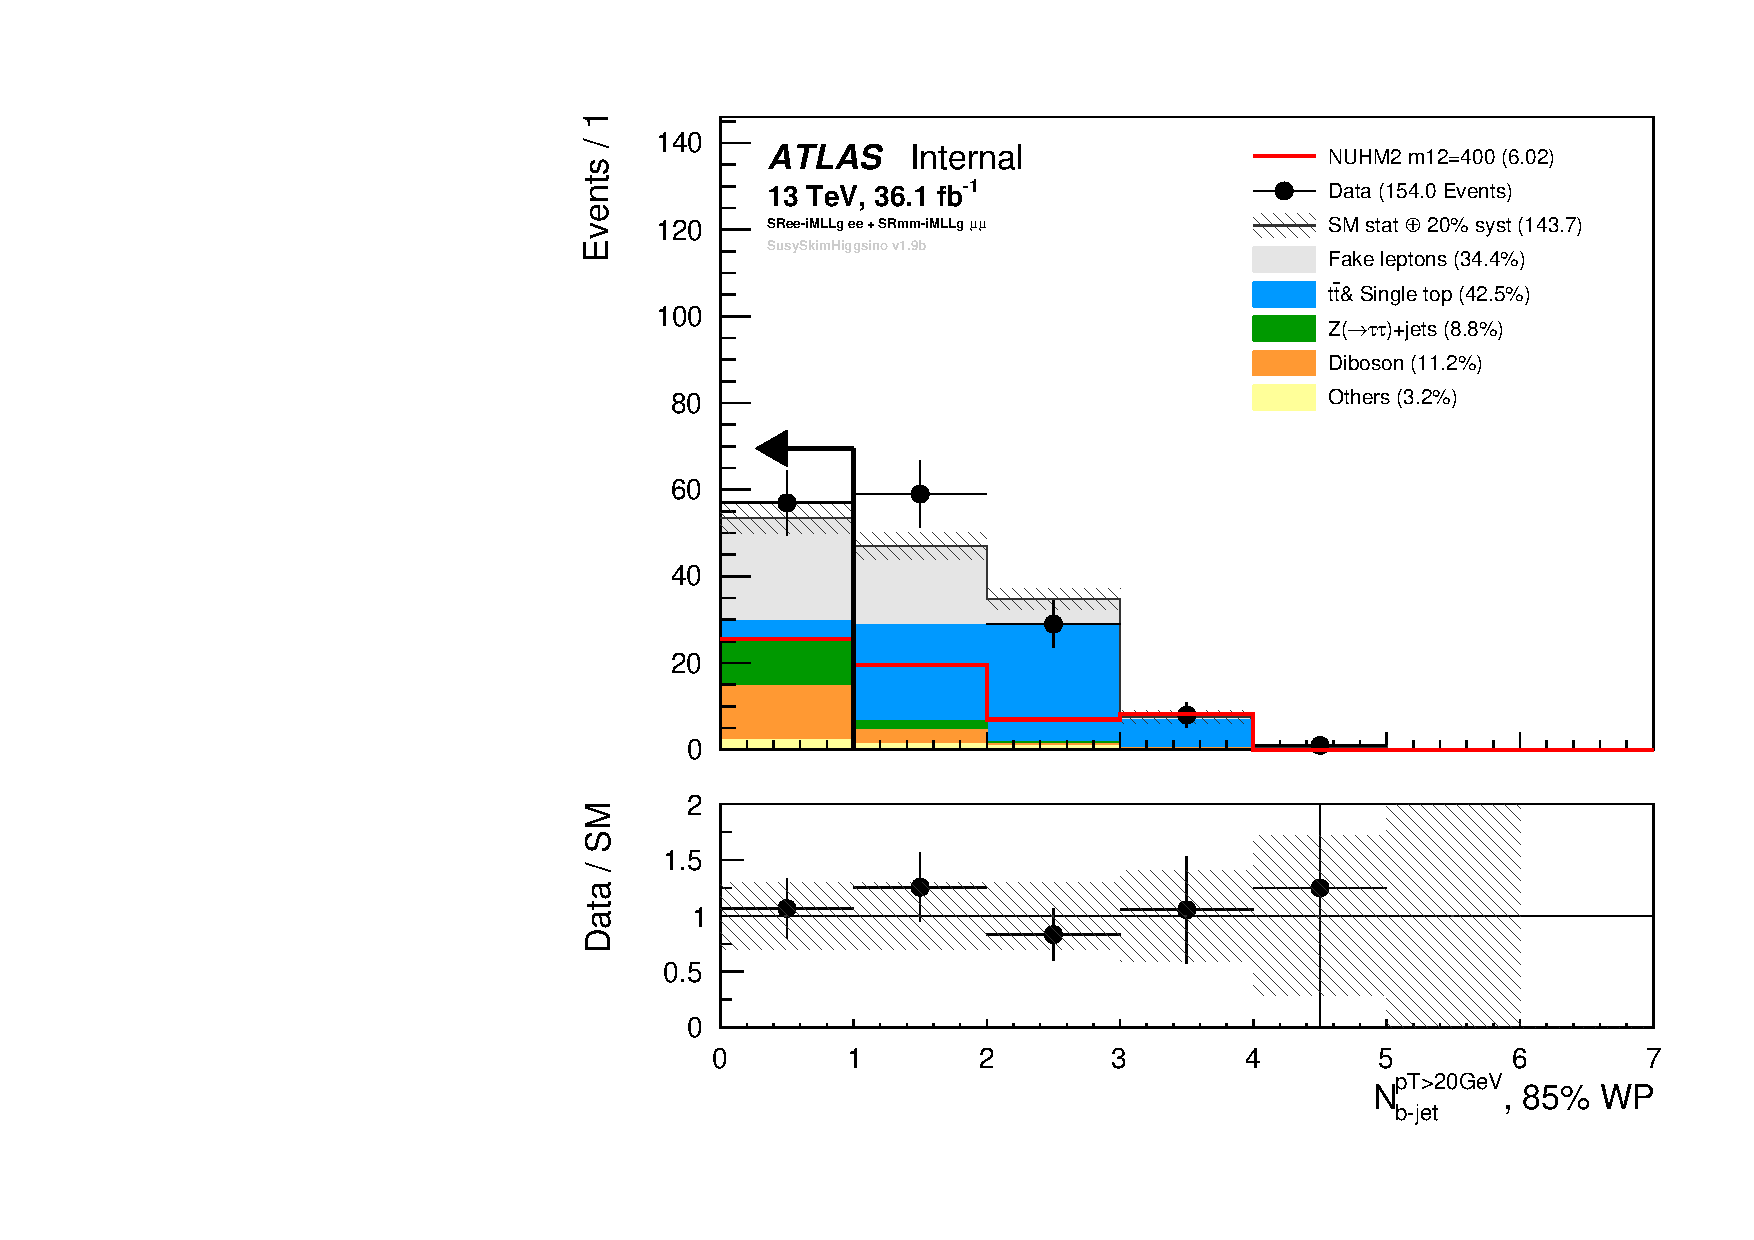
\includegraphics[scale=0.3]{NUHM2_m12_400_and_Bkg_nBJet20_MV2c10_SFOS_N_minus_one_distribution_in_SR_times_10_on_Nsig.pdf}
            \caption{$N^{20}_{\mathrm{b-jets}}$}
            \label{fig:event_nuhm2_m12_400_nBJet20_SFOS}
        \end{subfigure}
        \begin{subfigure}[b]{0.48\textwidth}
            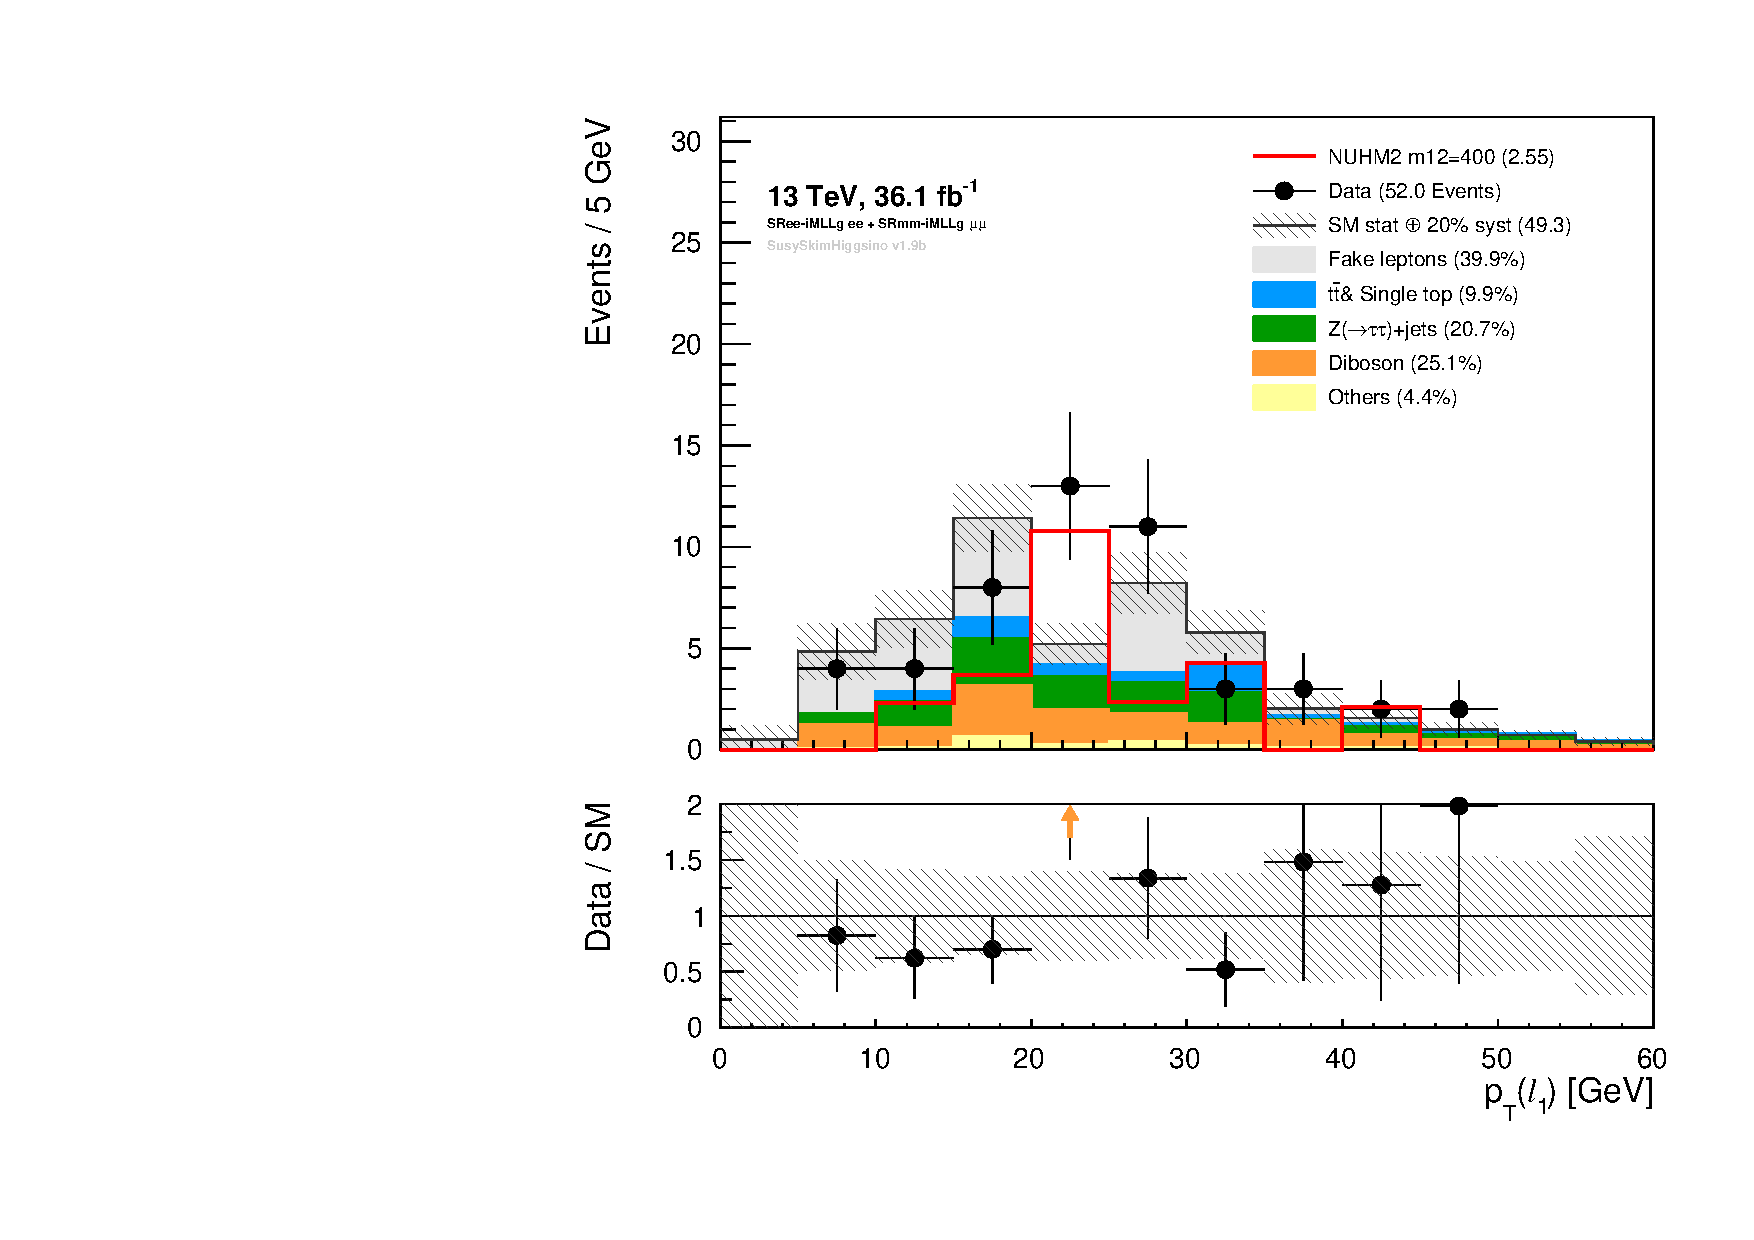
\includegraphics[scale=0.3]{NUHM2_m12_400_and_Bkg_lep1Pt_SFOS_N_minus_one_distribution_in_SR_times_10_on_Nsig.pdf}
            \caption{$p^{\ell_1}_{\mathrm{T}}$}
            \label{fig:event_nuhm2_m12_400_lep1Pt_SFOS}
        \end{subfigure}
        \begin{subfigure}[b]{0.48\textwidth}
            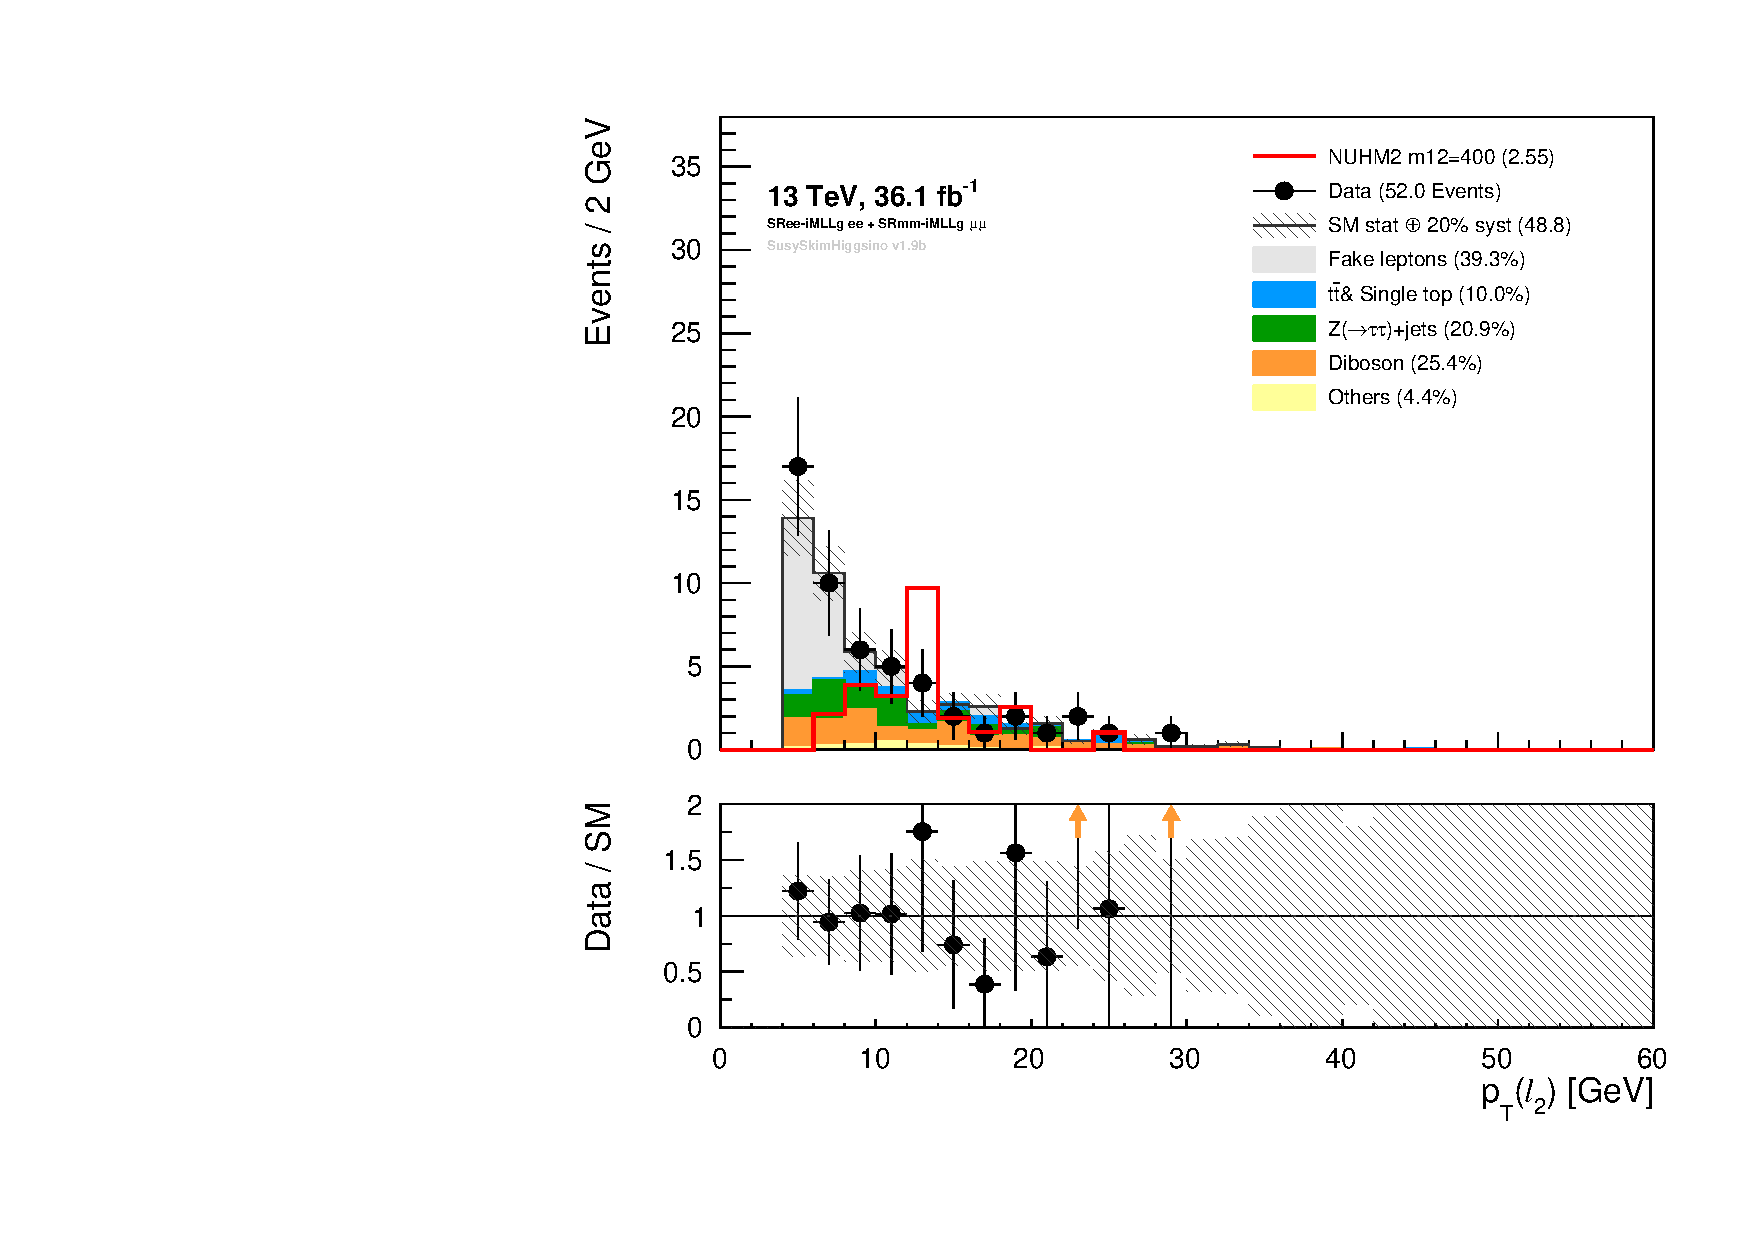
\includegraphics[scale=0.3]{NUHM2_m12_400_and_Bkg_lep2Pt_SFOS_N_minus_one_distribution_in_SR_times_10_on_Nsig.pdf}
            \caption{$p^{\ell_2}_{\mathrm{T}}$}
            \label{fig:event_nuhm2_m12_400_lep2Pt_SFOS}
        \end{subfigure}
        \begin{subfigure}[b]{0.48\textwidth}
            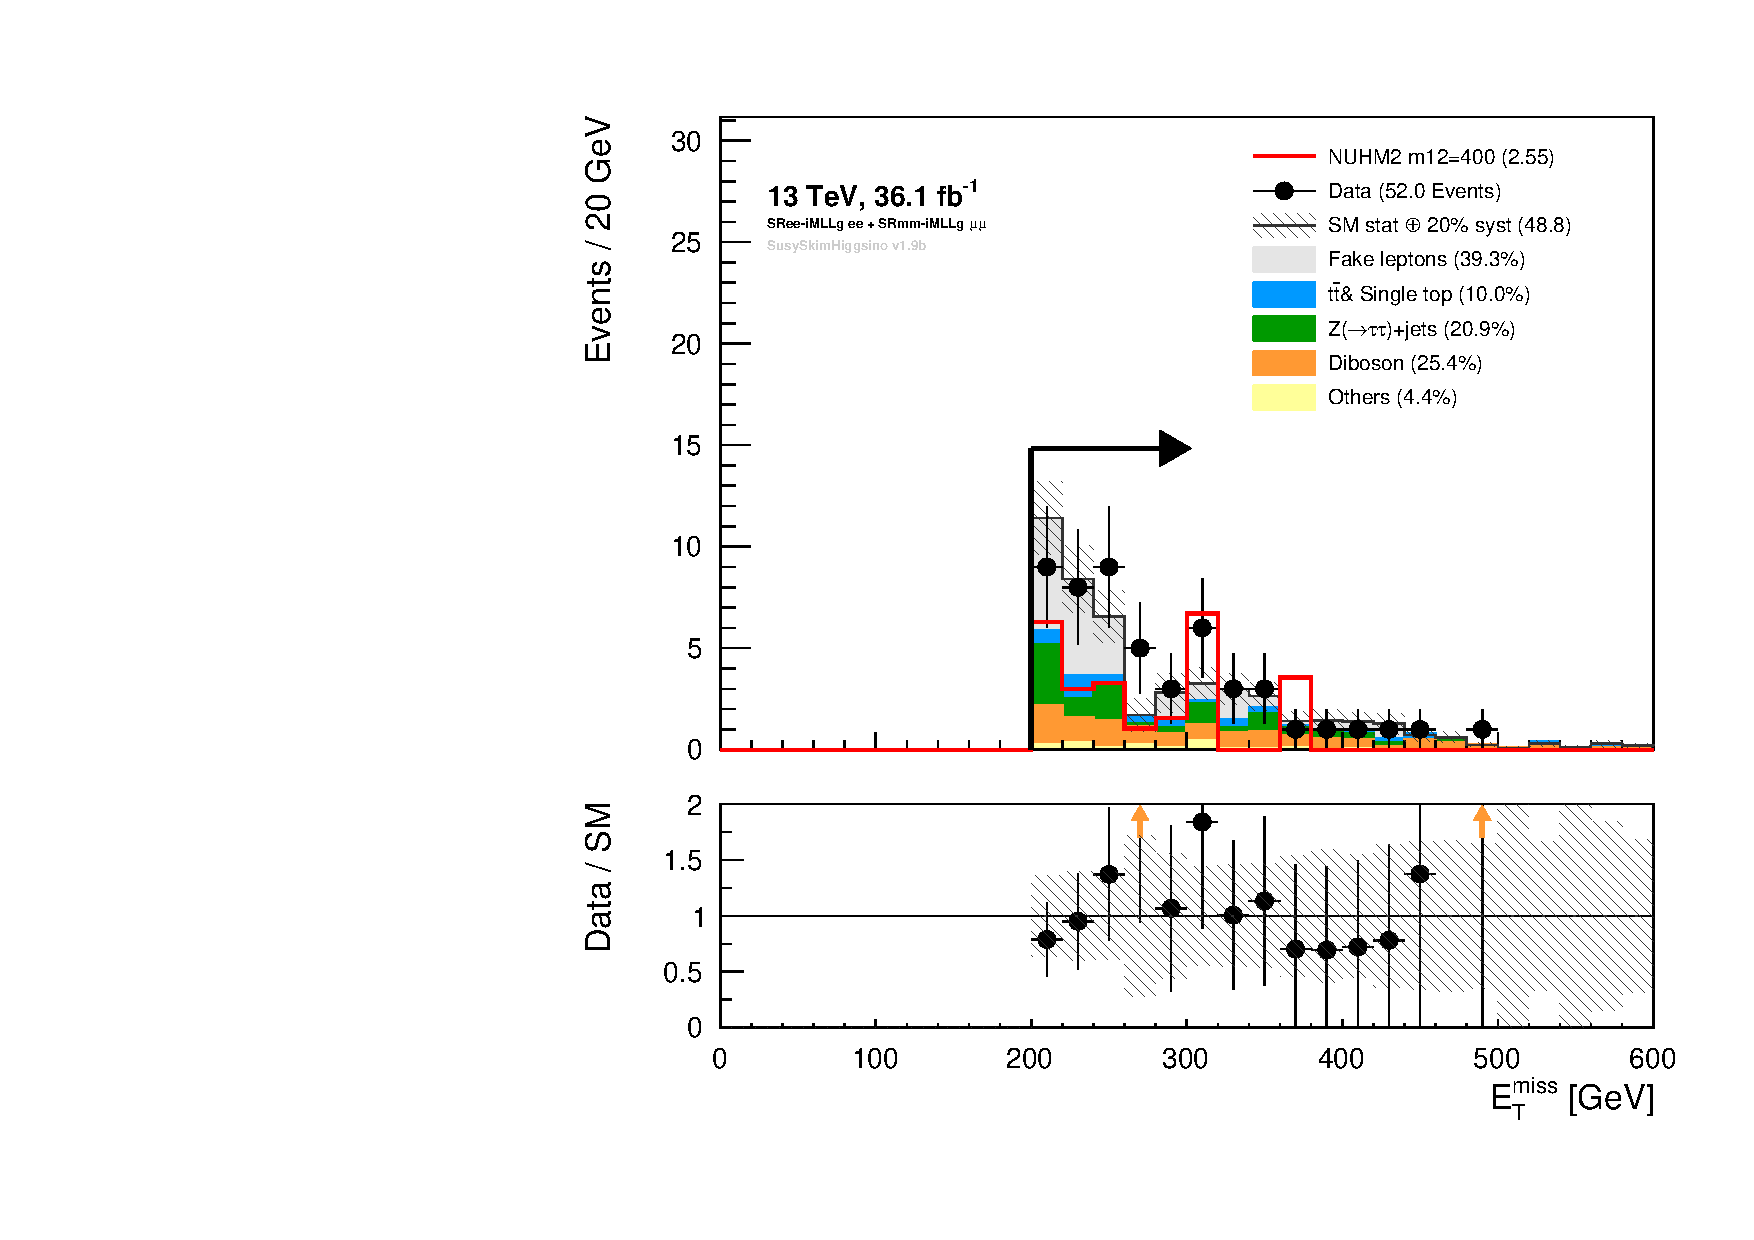
\includegraphics[scale=0.3]{NUHM2_m12_400_and_Bkg_met_Et_SFOS_N_minus_one_distribution_in_SR_times_10_on_Nsig.pdf}
            \caption{$E^{\mathrm{miss}}_{\mathrm{T}}$}
            \label{fig:event_nuhm2_m12_400_met_SFOS}
        \end{subfigure}
        \begin{subfigure}[b]{0.48\textwidth}
            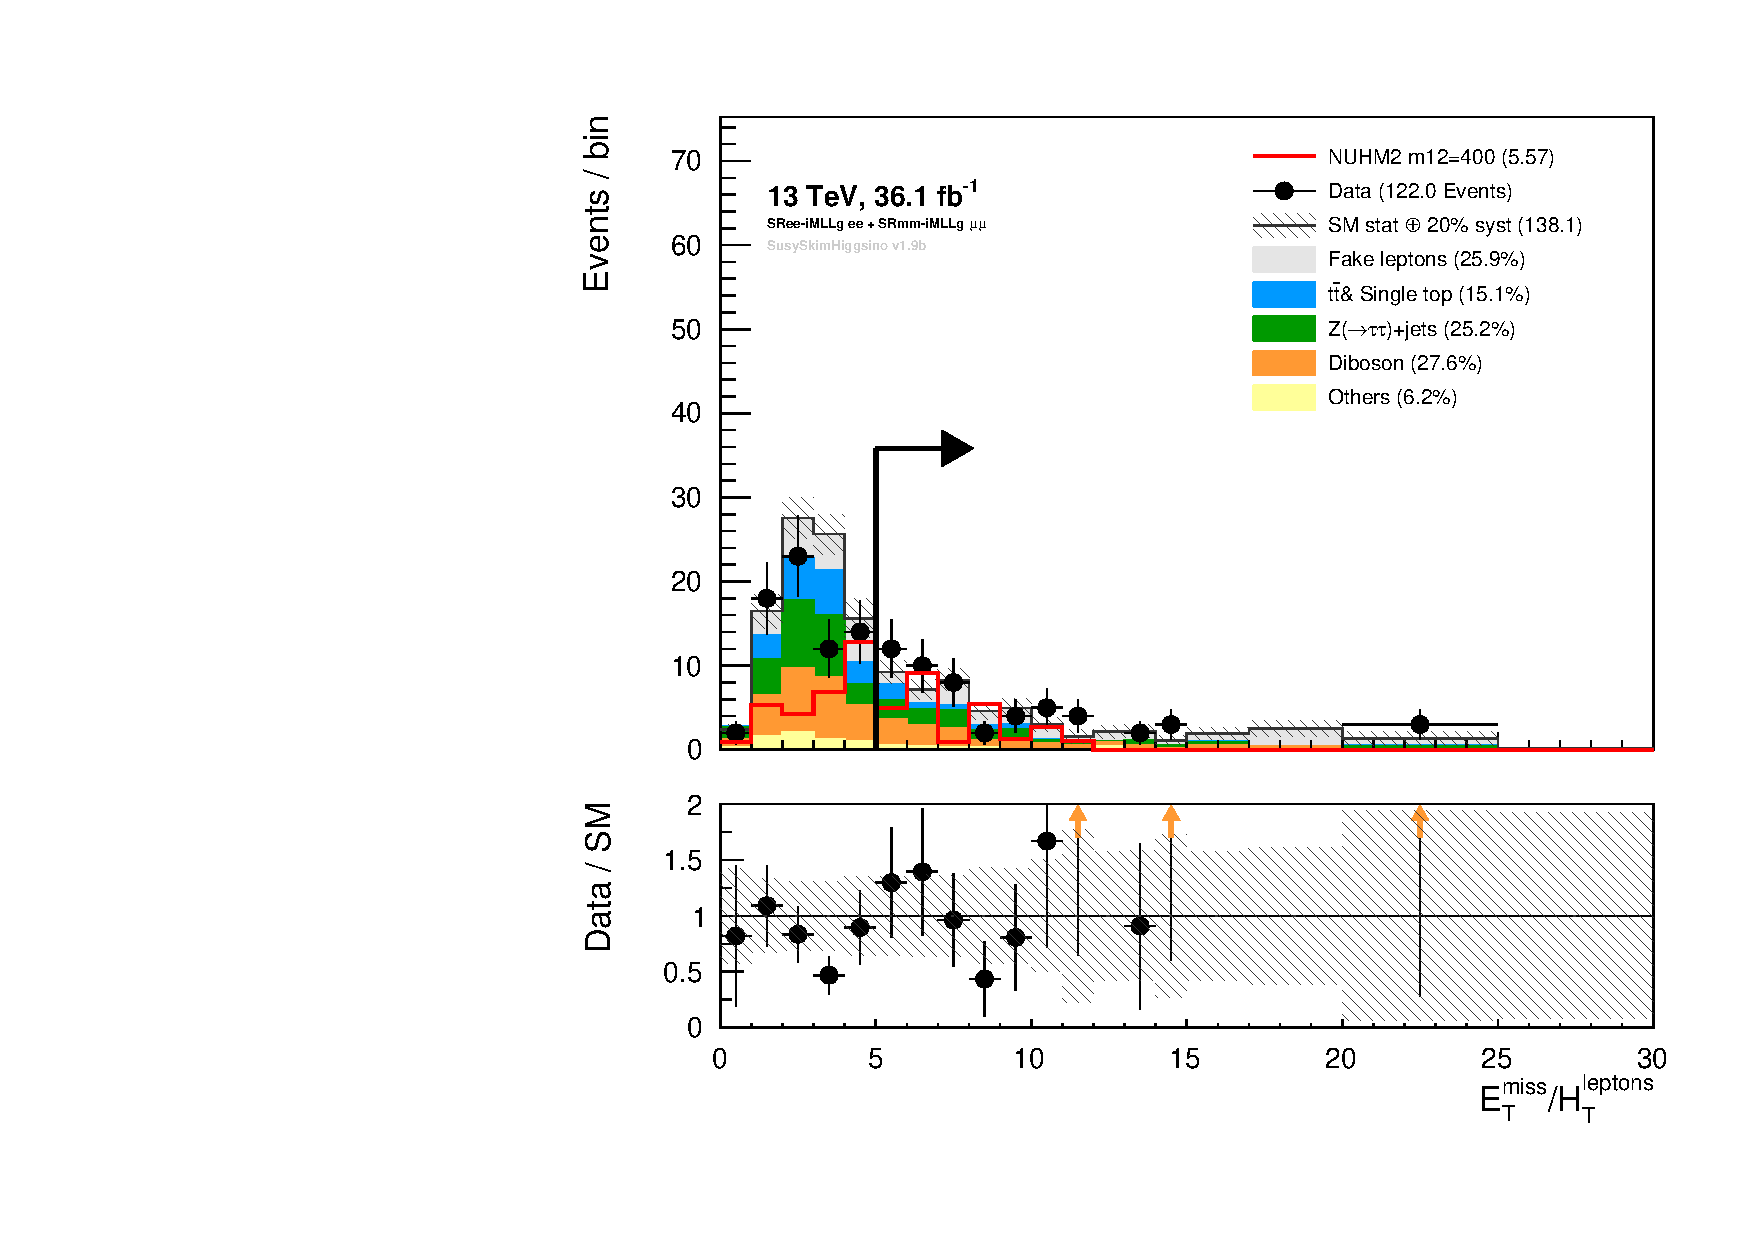
\includegraphics[scale=0.3]{NUHM2_m12_400_and_Bkg_METOverHTLep_SFOS_N_minus_one_distribution_in_SR_times_10_on_Nsig.pdf}
            \caption{$E^{\mathrm{miss}}_{\mathrm{T}} / H^{\mathrm{leptons}}_{\mathrm{T}}$}
            \label{fig:event_nuhm2_m12_400_METOverHTLep_SFOS}
        \end{subfigure}
    \end{center}
    \caption{The `$N-1$' distributions for NUHM2 model with $m_{1/2} = 400$~{\GeV} in SR region $1 < $SR$\ell \ell$-$m_{\ell \ell} < 60$~{\GeV}.
    The NUHM2 distributions are multiplied by 10 but the number of events in the legend use its actual values.}
    \label{fig:event_nuhm2_kinematic_in_SR_SFOS_m12_400_1}
\end{figure}

\begin{figure}[htbp]
    \begin{center}
        \begin{subfigure}[b]{0.48\textwidth}
            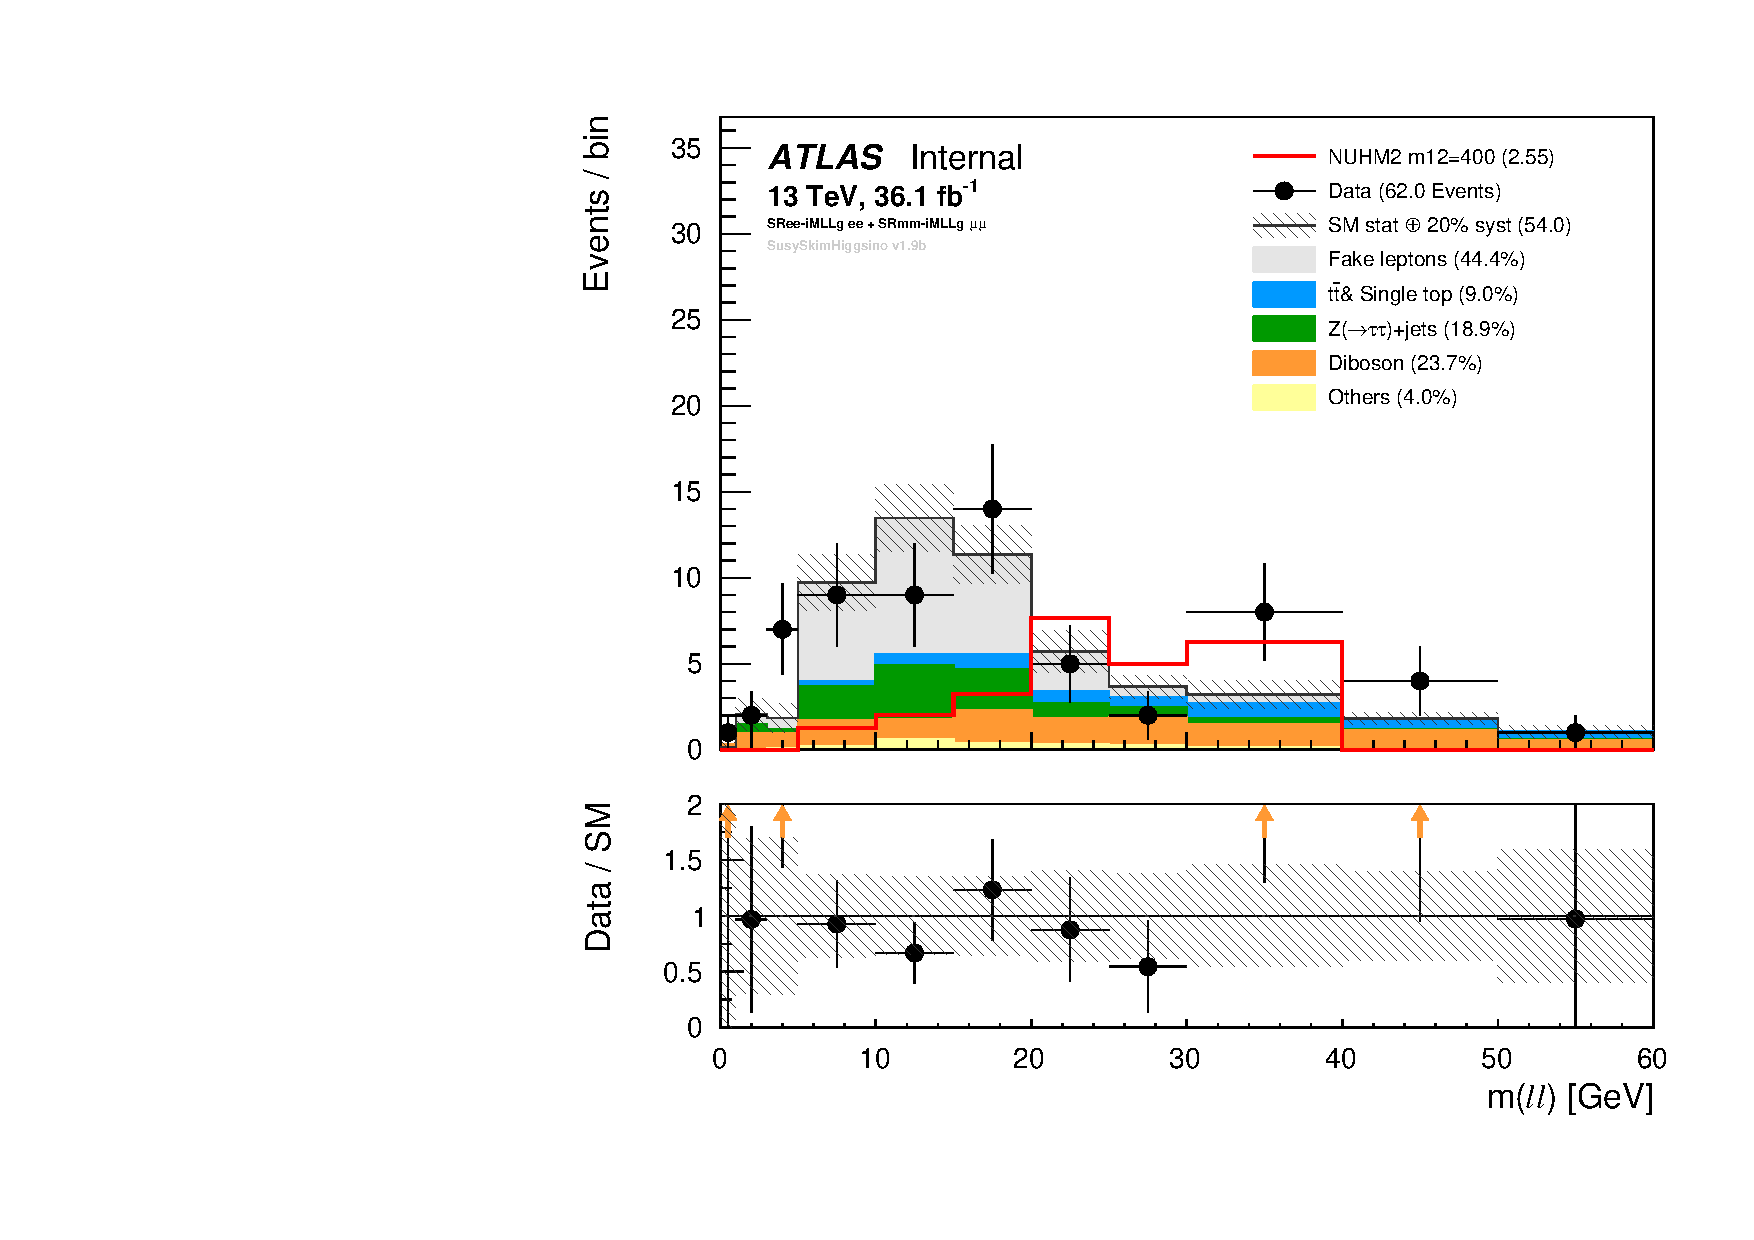
\includegraphics[scale=0.3]{NUHM2_m12_400_and_Bkg_mll_SFOS_N_minus_one_distribution_in_SR_times_10_on_Nsig.pdf}
            \caption{$m_{\ell\ell}$}
            \label{fig:event_nuhm2_m12_400_mll_SFOS}
        \end{subfigure}
        \begin{subfigure}[b]{0.48\textwidth}
            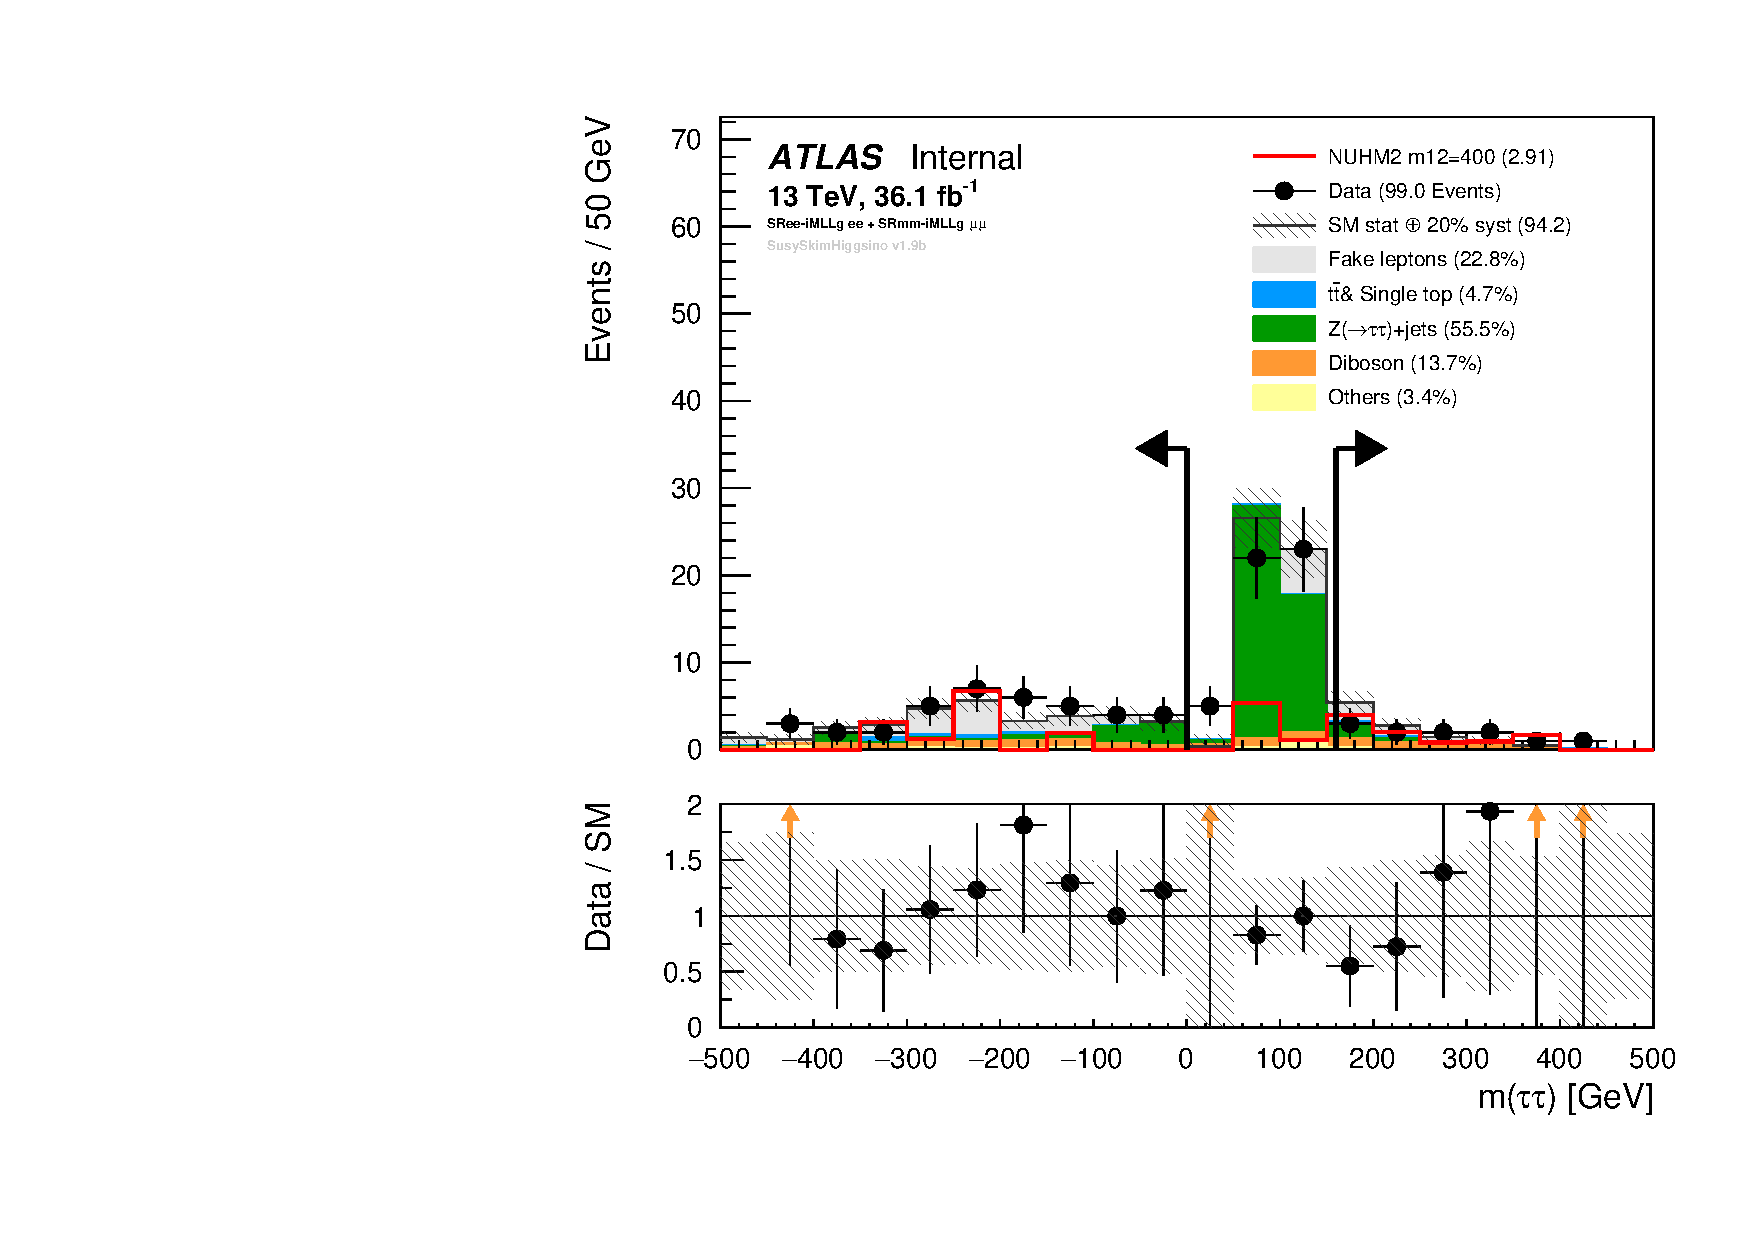
\includegraphics[scale=0.3]{NUHM2_m12_400_and_Bkg_MTauTau_SFOS_N_minus_one_distribution_in_SR_times_10_on_Nsig.pdf}
            \caption{$m_{\tau\tau}$}
            \label{fig:event_nuhm2_m12_400_MTauTau_SFOS}
        \end{subfigure}
        \begin{subfigure}[b]{0.48\textwidth}
            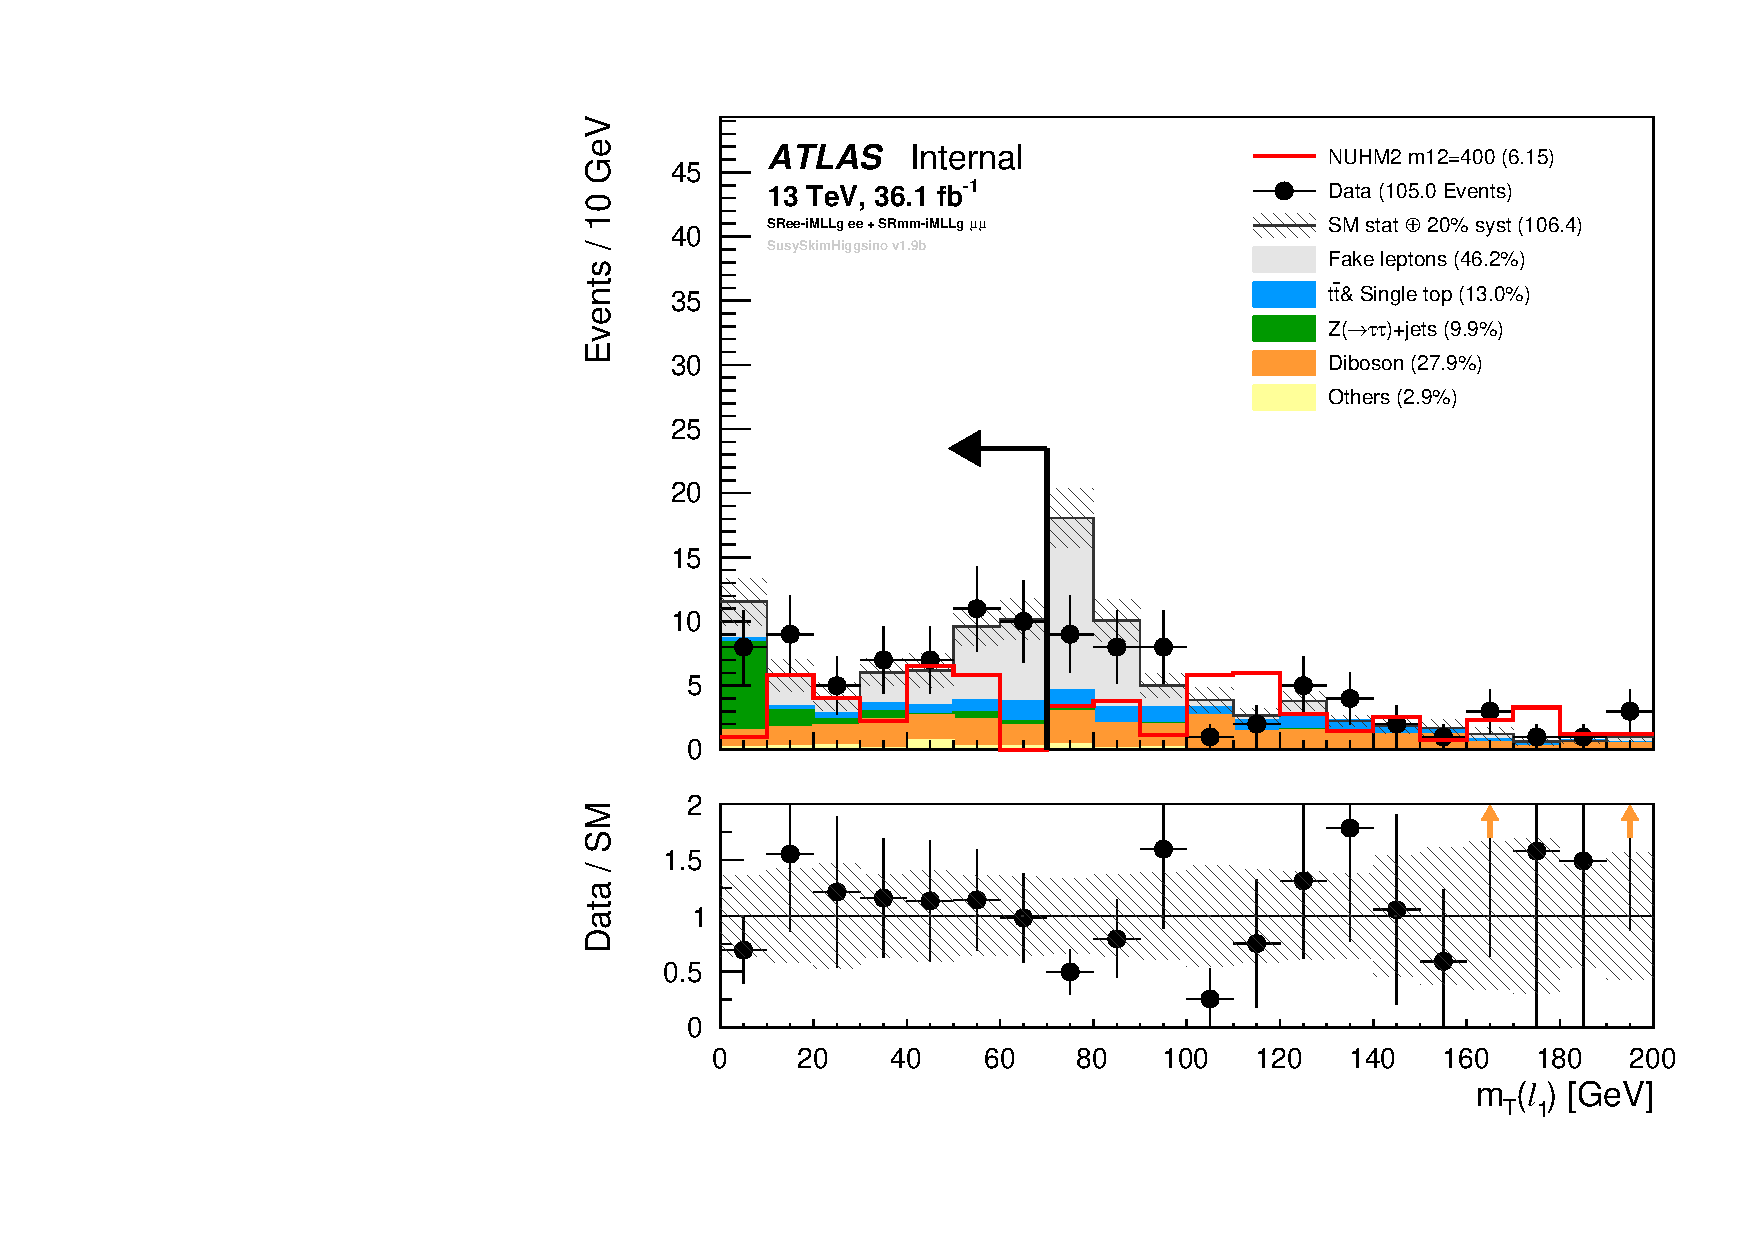
\includegraphics[scale=0.3]{NUHM2_m12_400_and_Bkg_mt_lep1_SFOS_N_minus_one_distribution_in_SR_times_10_on_Nsig.pdf}
            \caption{$m_{T}(\ell_{1})$}
            \label{fig:event_nuhm2_m12_400_mt_lep1_SFOS}
        \end{subfigure}
        \begin{subfigure}[b]{0.48\textwidth}
            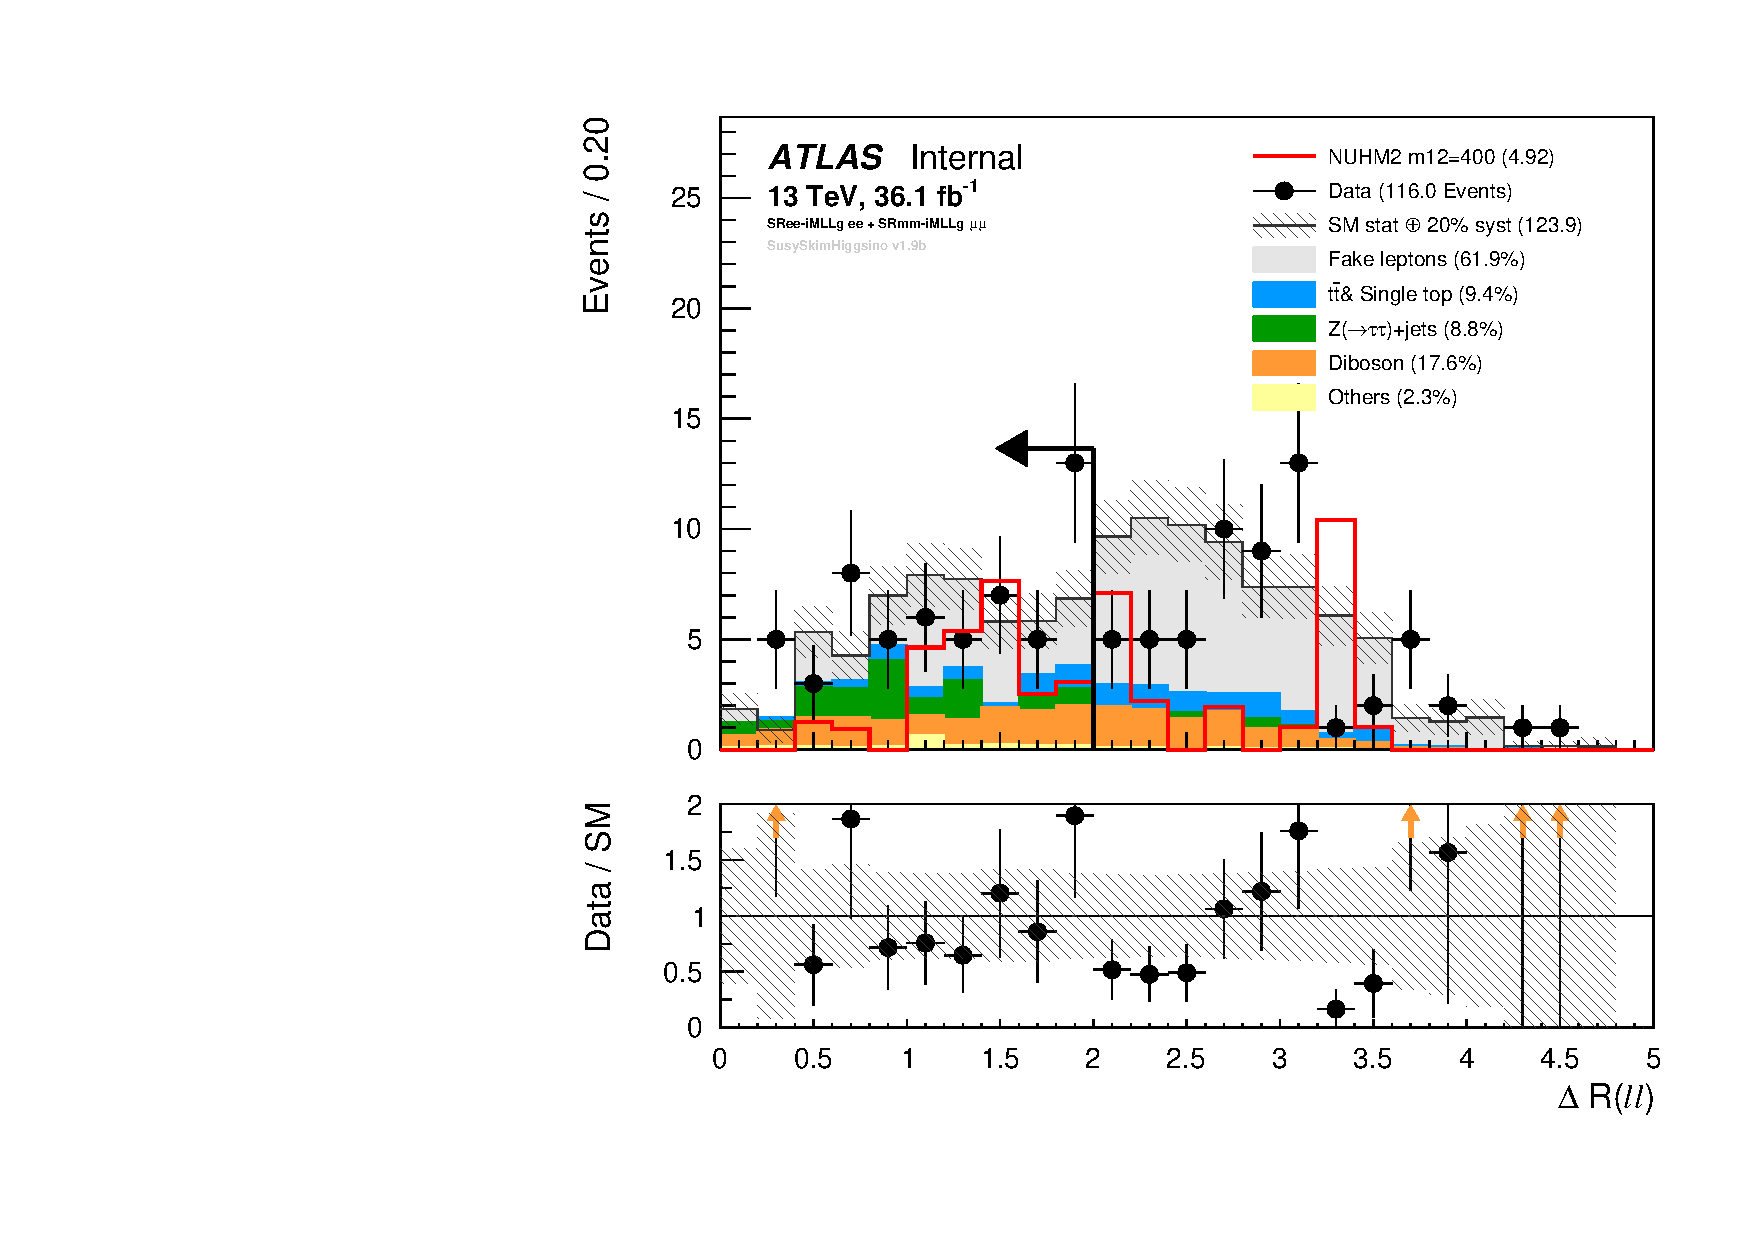
\includegraphics[scale=0.3]{NUHM2_m12_400_and_Bkg_Rll_SFOS_N_minus_one_distribution_in_SR_times_10_on_Nsig.pdf}
            \caption{$\Delta R_{\ell\ell}$}
            \label{fig:event_nuhm2_m12_400_Rll_SFOS}
        \end{subfigure}
        \begin{subfigure}[b]{0.48\textwidth}
            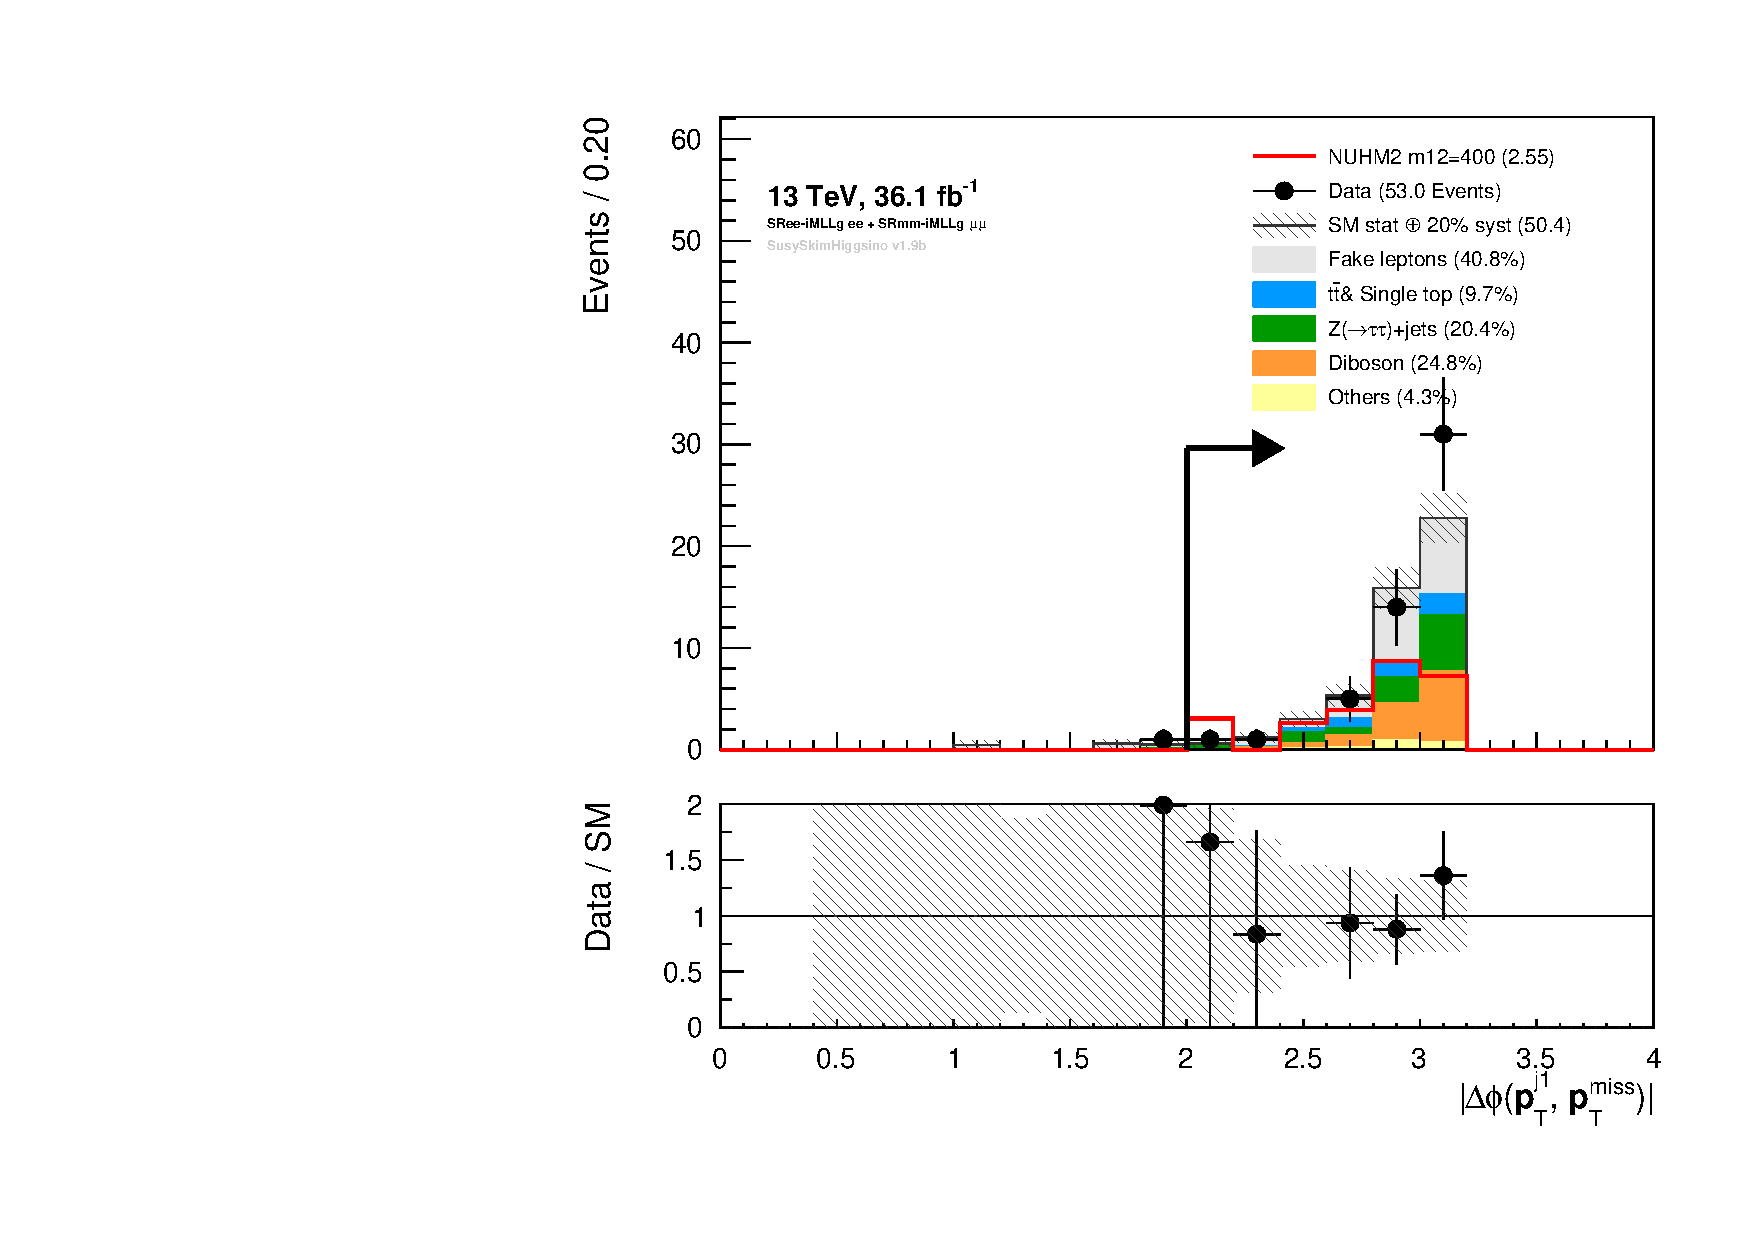
\includegraphics[scale=0.3]{NUHM2_m12_400_and_Bkg_DPhiJ1Met_SFOS_N_minus_one_distribution_in_SR_times_10_on_Nsig.pdf}
            \caption{$|\Delta \phi(\mathbf{p}^{j_{1}}_{\mathrm{T}}, \mathbf{p}^{\mathrm{miss}}_{\mathrm{T}})|$}
            \label{fig:event_nuhm2_m12_400_DPhiJ1Met_SFOS}
        \end{subfigure}
        \begin{subfigure}[b]{0.48\textwidth}
            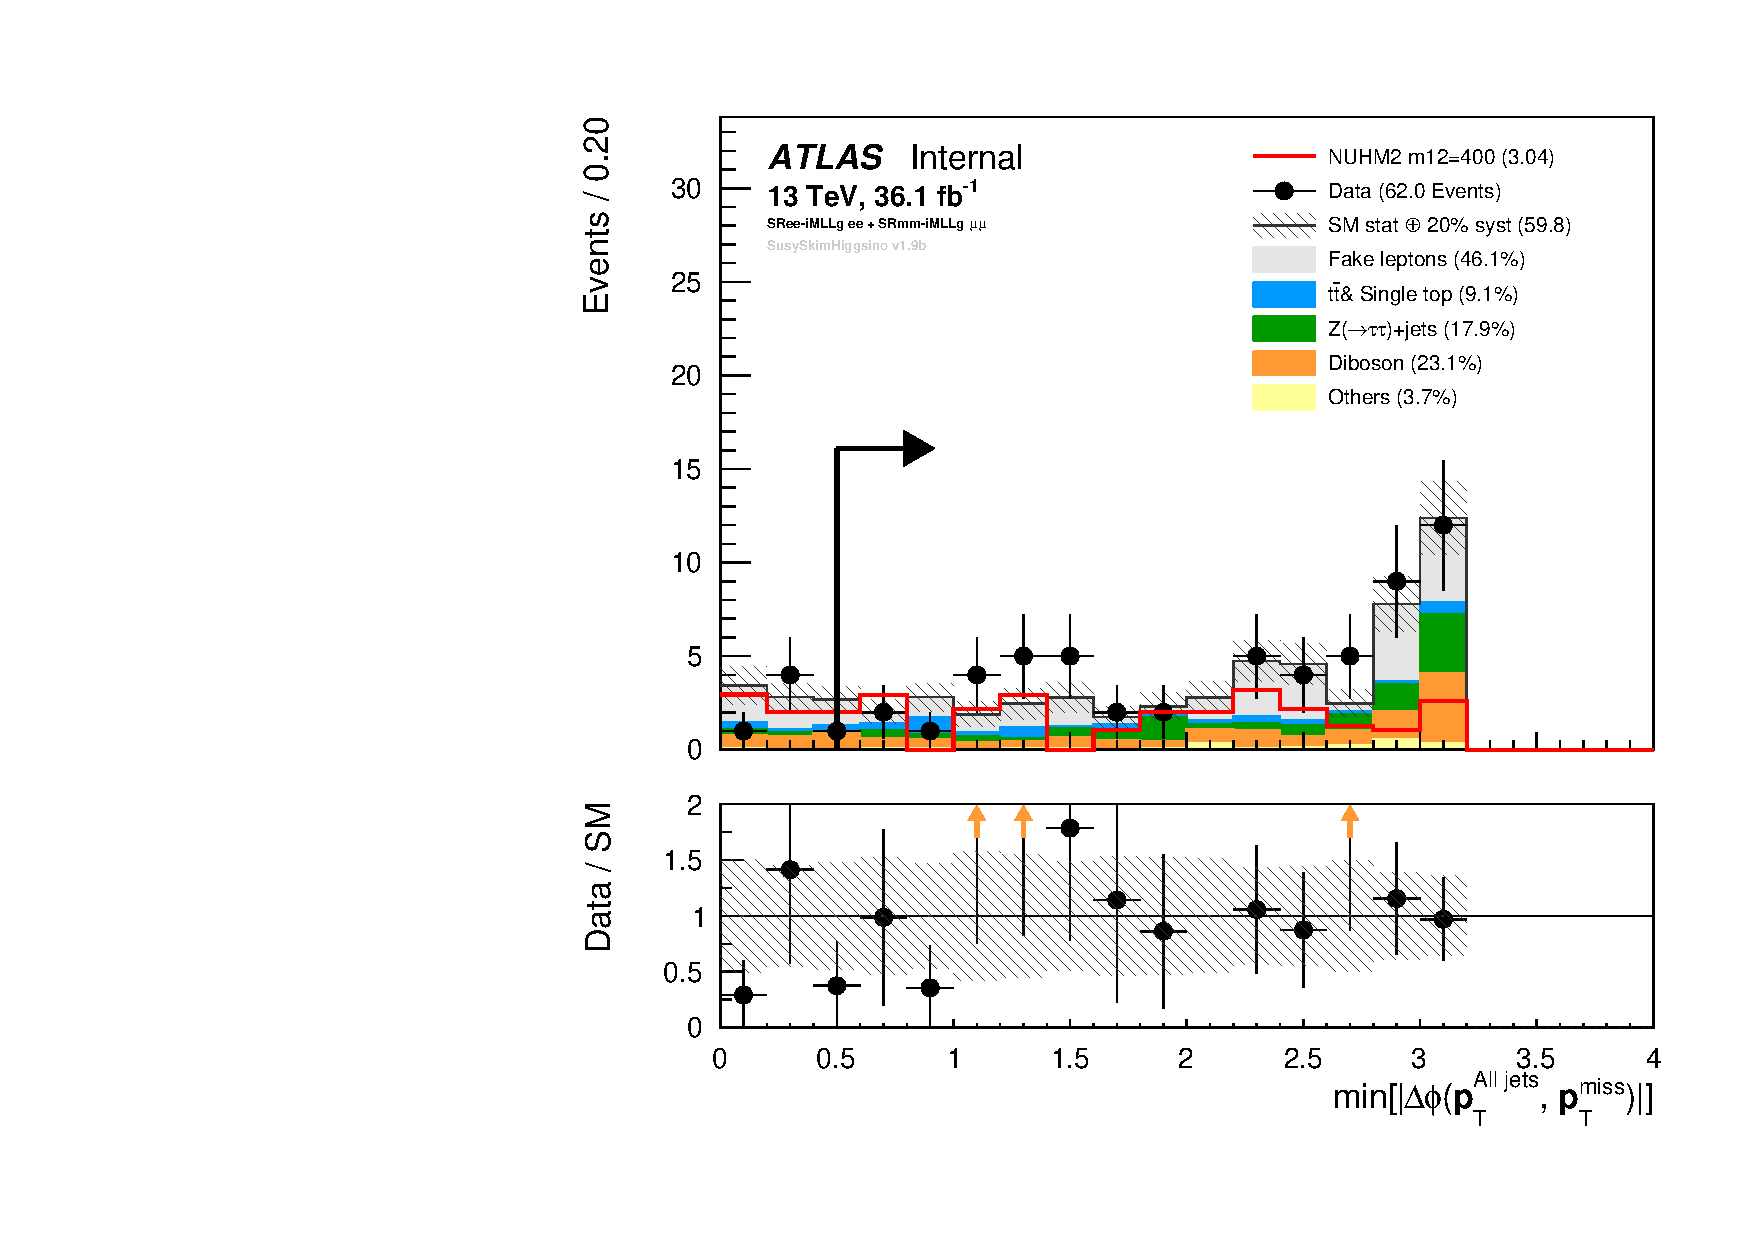
\includegraphics[scale=0.3]{NUHM2_m12_400_and_Bkg_minDPhiAllJetsMet_SFOS_N_minus_one_distribution_in_SR_times_10_on_Nsig.pdf}
            \caption{min[$|\Delta \phi(\mathbf{p}^{\textrm{All jets}}_{\mathrm{T}}, \mathbf{p}^{\mathrm{miss}}_{\mathrm{T}})|$]}
            \label{fig:event_nuhm2_m12_400_minDPhiAllJetsMet_SFOS}
        \end{subfigure}
    \end{center}
    \caption{The `$N-1$' distributions for NUHM2 model with $m_{1/2} = 400$~{\GeV} in SR region $1 < $SR$\ell \ell$-$m_{\ell \ell} < 60$~{\GeV}.
    The NUHM2 distributions are multiplied by 10 but the number of events in the legend use its actual values.}
    \label{fig:event_nuhm2_kinematic_in_SR_SFOS_m12_400_2}
\end{figure}

% m12 = 500
\begin{figure}[htbp]
    \begin{center}
        \begin{subfigure}[b]{0.48\textwidth}
            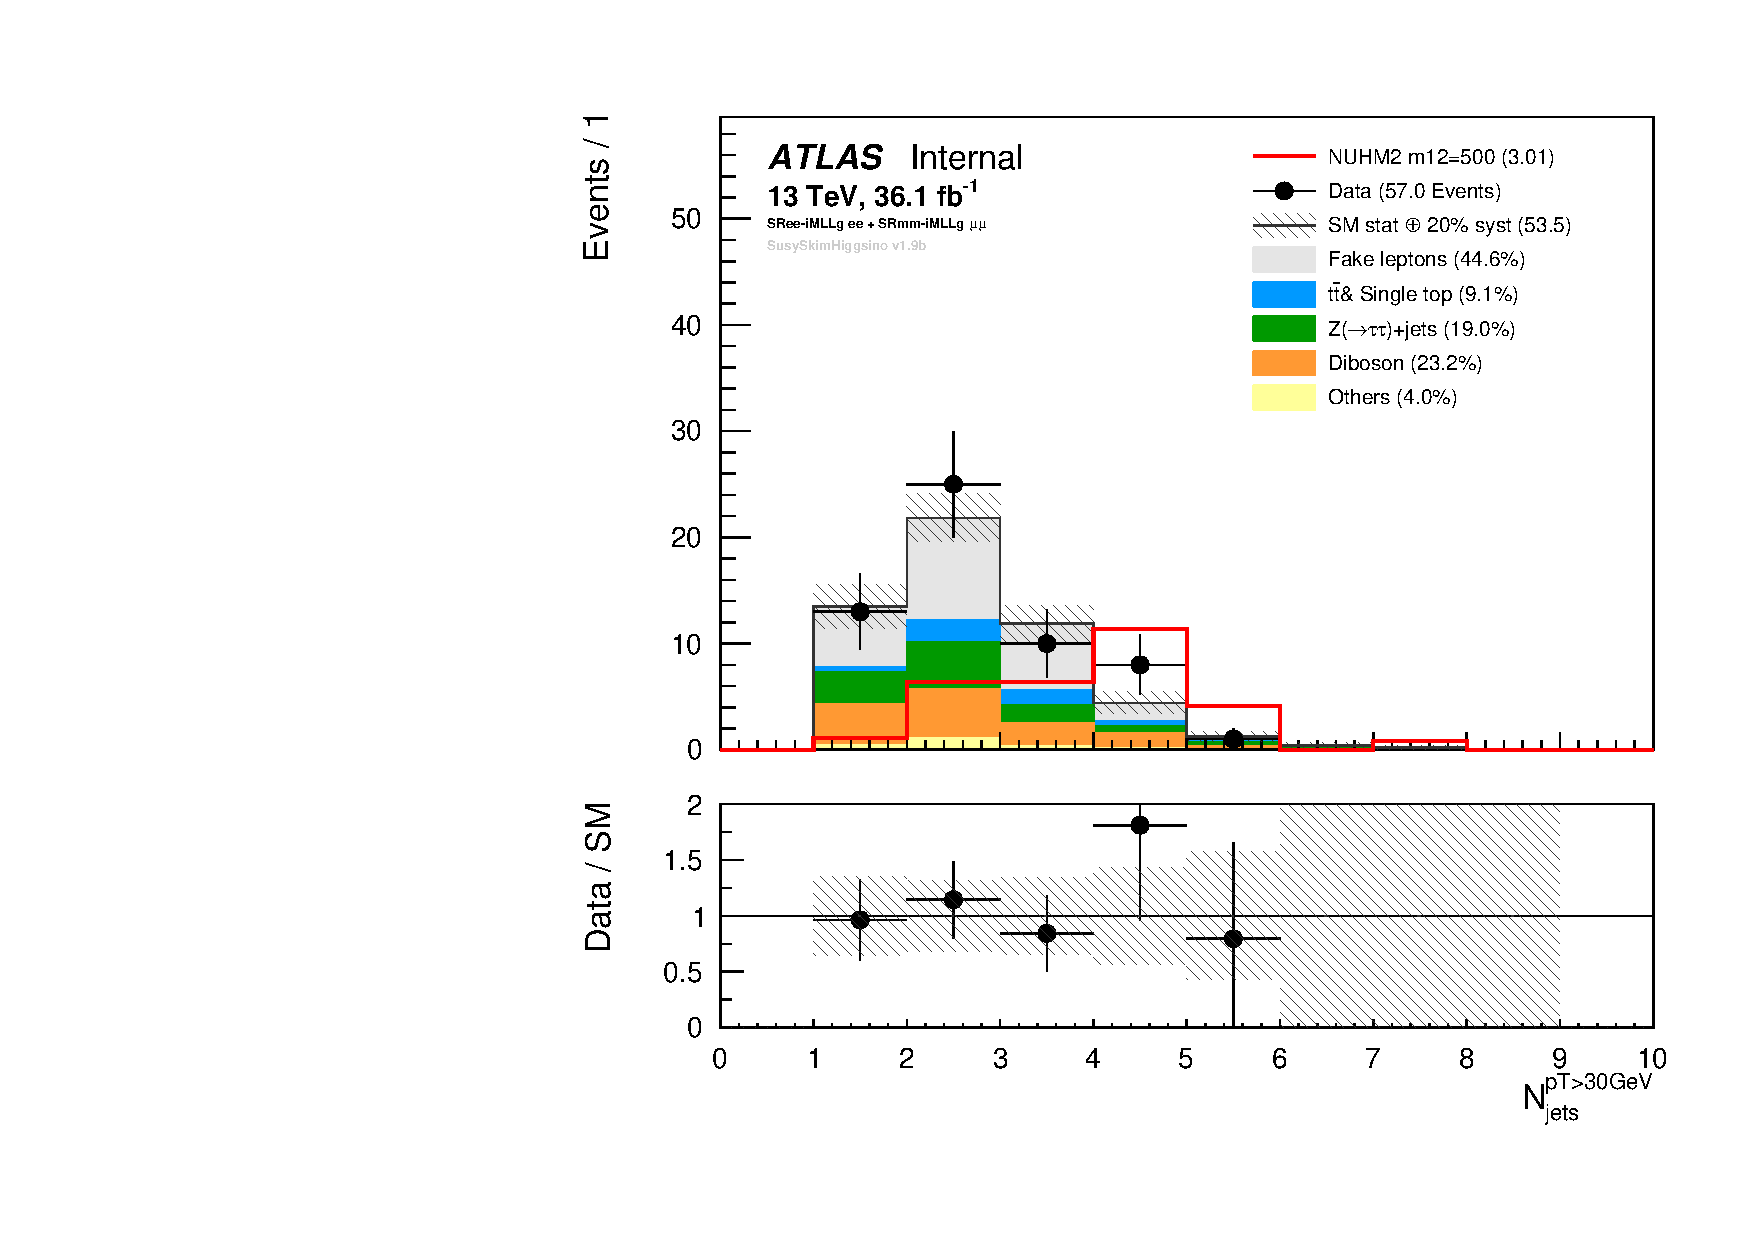
\includegraphics[scale=0.3]{NUHM2_m12_500_and_Bkg_nJet30_SFOS_N_minus_one_distribution_in_SR_times_10_on_Nsig.pdf}
            \caption{$N^{30}_{\mathrm{jets}}$}
            \label{fig:event_nuhm2_m12_500_nJet30_SFOS}
        \end{subfigure}
        \begin{subfigure}[b]{0.48\textwidth}
            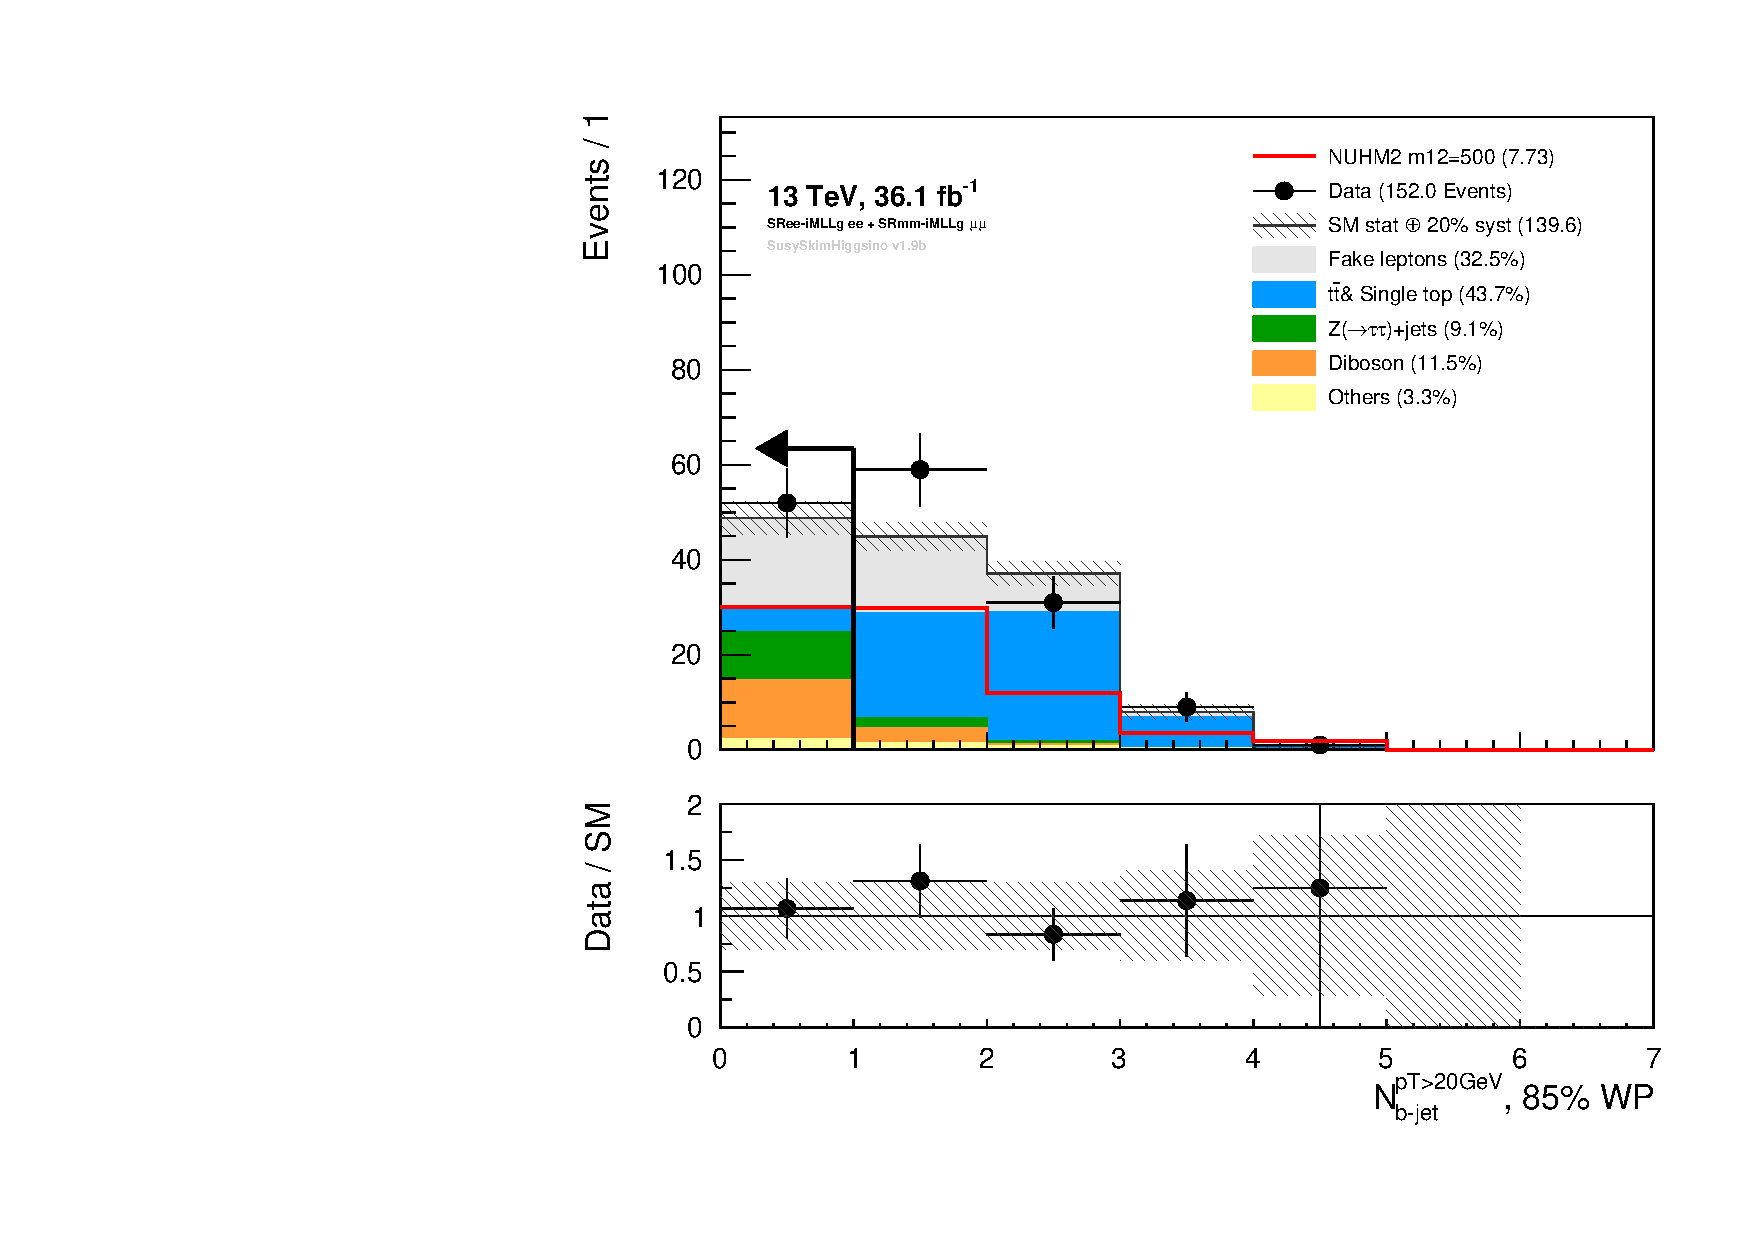
\includegraphics[scale=0.3]{NUHM2_m12_500_and_Bkg_nBJet20_MV2c10_SFOS_N_minus_one_distribution_in_SR_times_10_on_Nsig.pdf}
            \caption{$N^{20}_{\mathrm{b-jets}}$}
            \label{fig:event_nuhm2_m12_500_nBJet20_SFOS}
        \end{subfigure}
        \begin{subfigure}[b]{0.48\textwidth}
            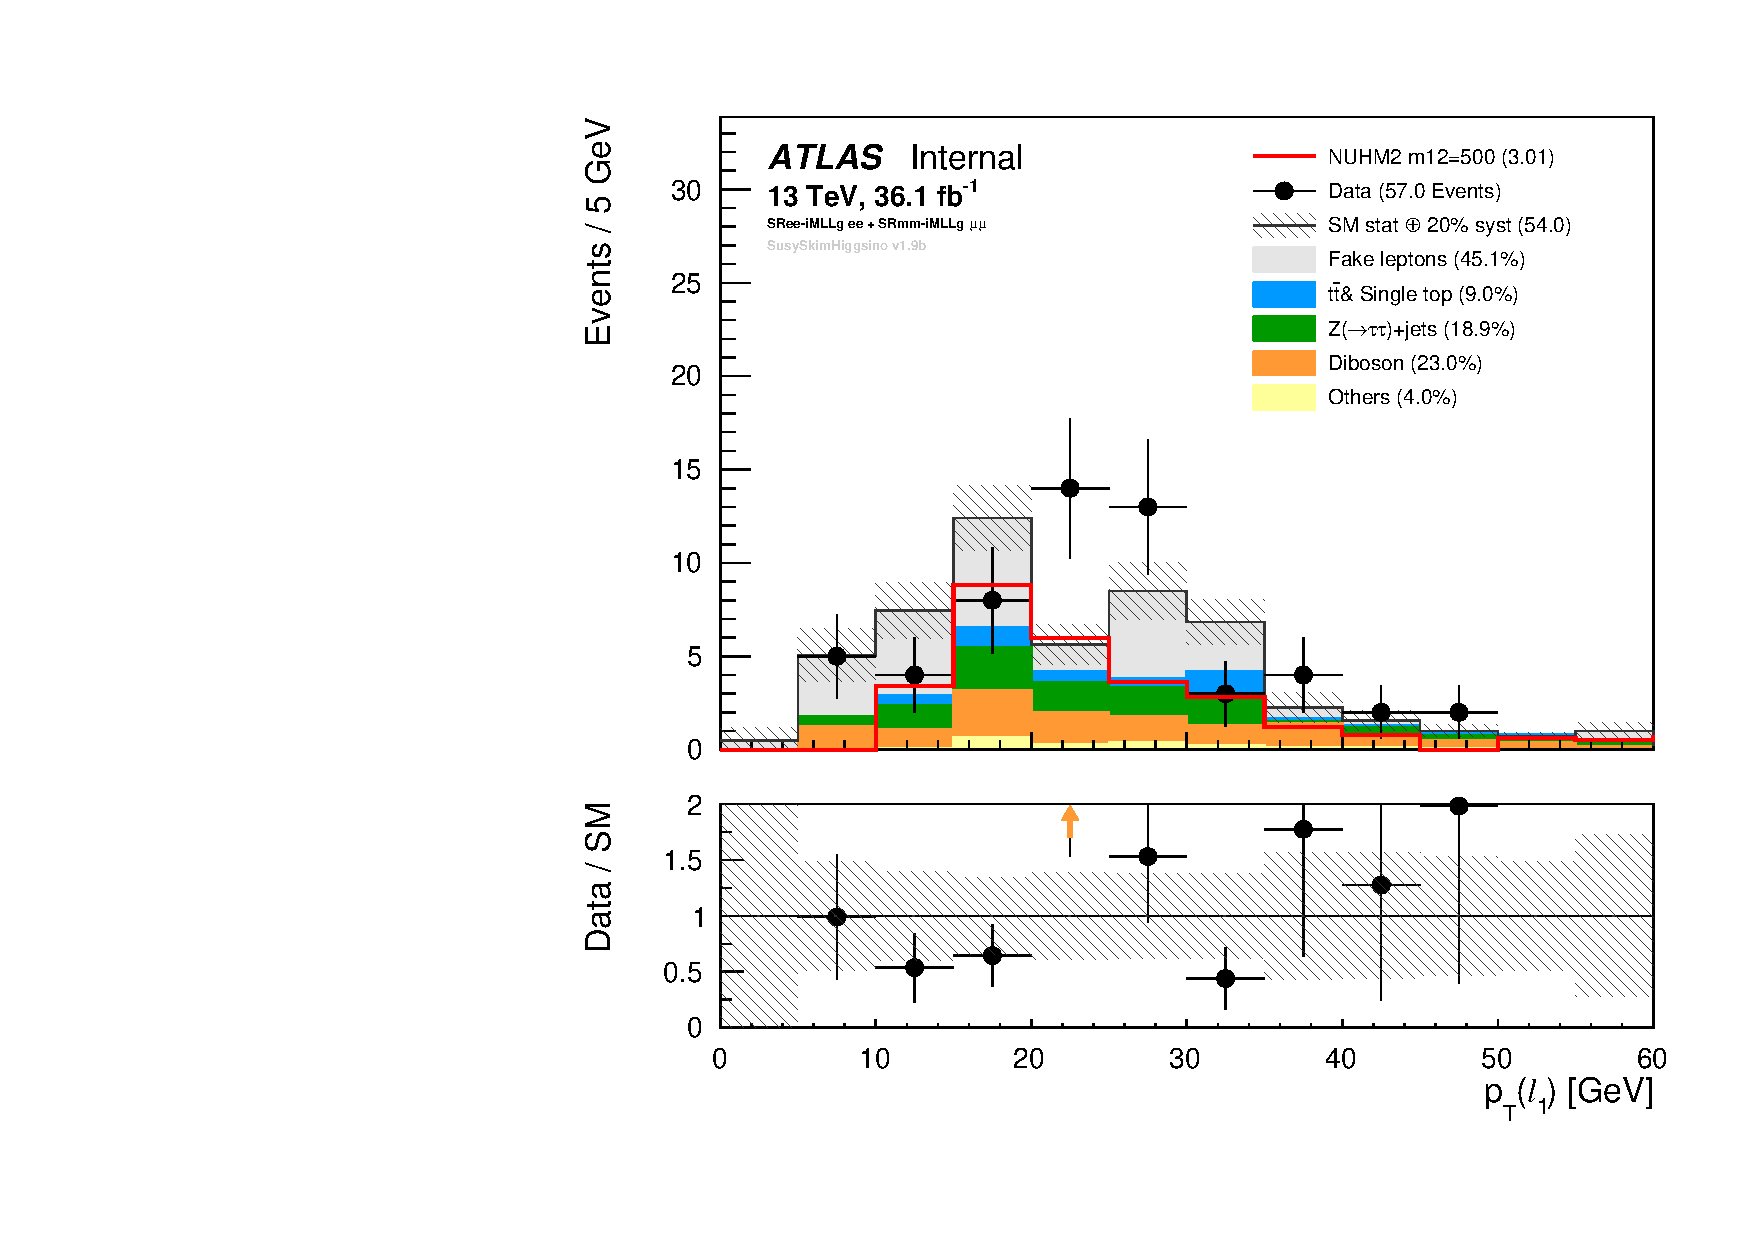
\includegraphics[scale=0.3]{NUHM2_m12_500_and_Bkg_lep1Pt_SFOS_N_minus_one_distribution_in_SR_times_10_on_Nsig.pdf}
            \caption{$p^{\ell_1}_{\mathrm{T}}$}
            \label{fig:event_nuhm2_m12_500_lep1Pt_SFOS}
        \end{subfigure}
        \begin{subfigure}[b]{0.48\textwidth}
            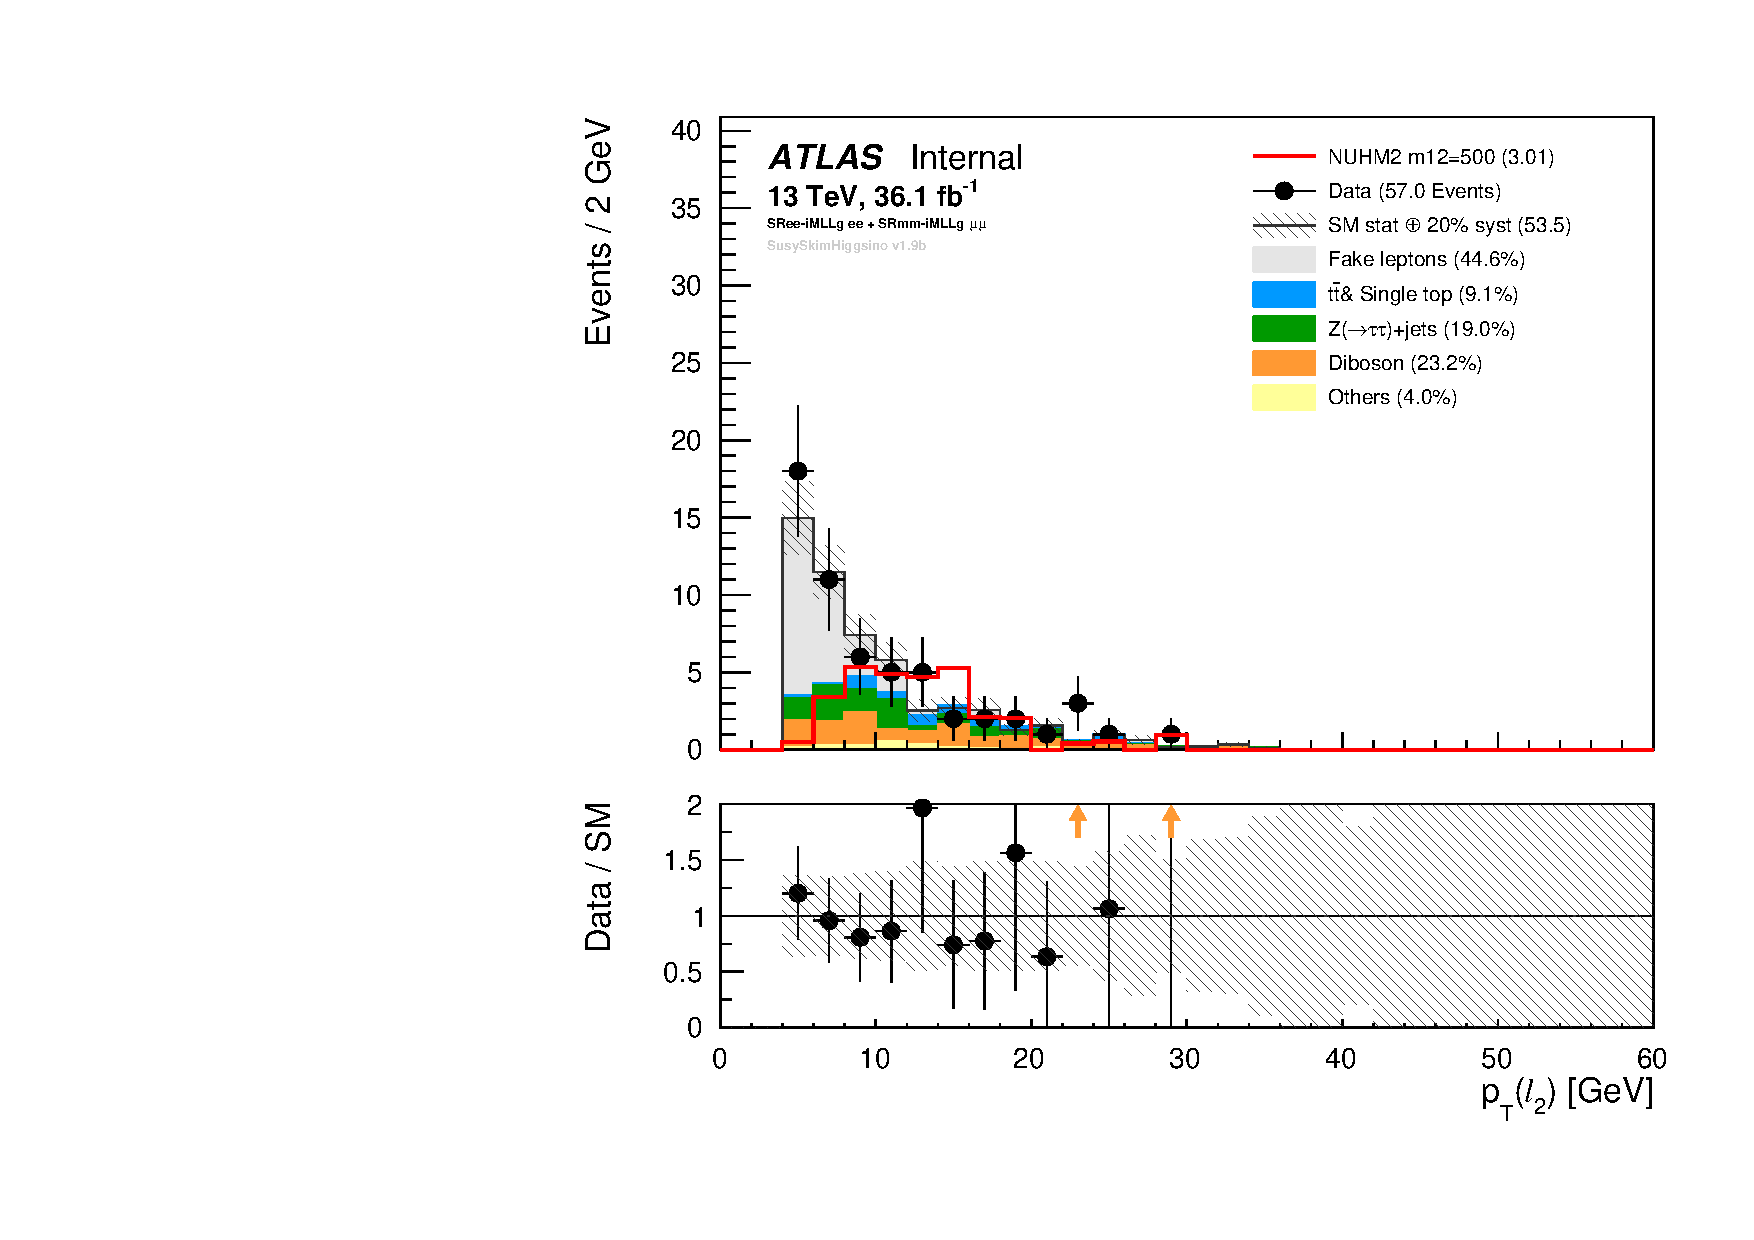
\includegraphics[scale=0.3]{NUHM2_m12_500_and_Bkg_lep2Pt_SFOS_N_minus_one_distribution_in_SR_times_10_on_Nsig.pdf}
            \caption{$p^{\ell_2}_{\mathrm{T}}$}
            \label{fig:event_nuhm2_m12_500_lep2Pt_SFOS}
        \end{subfigure}
        \begin{subfigure}[b]{0.48\textwidth}
            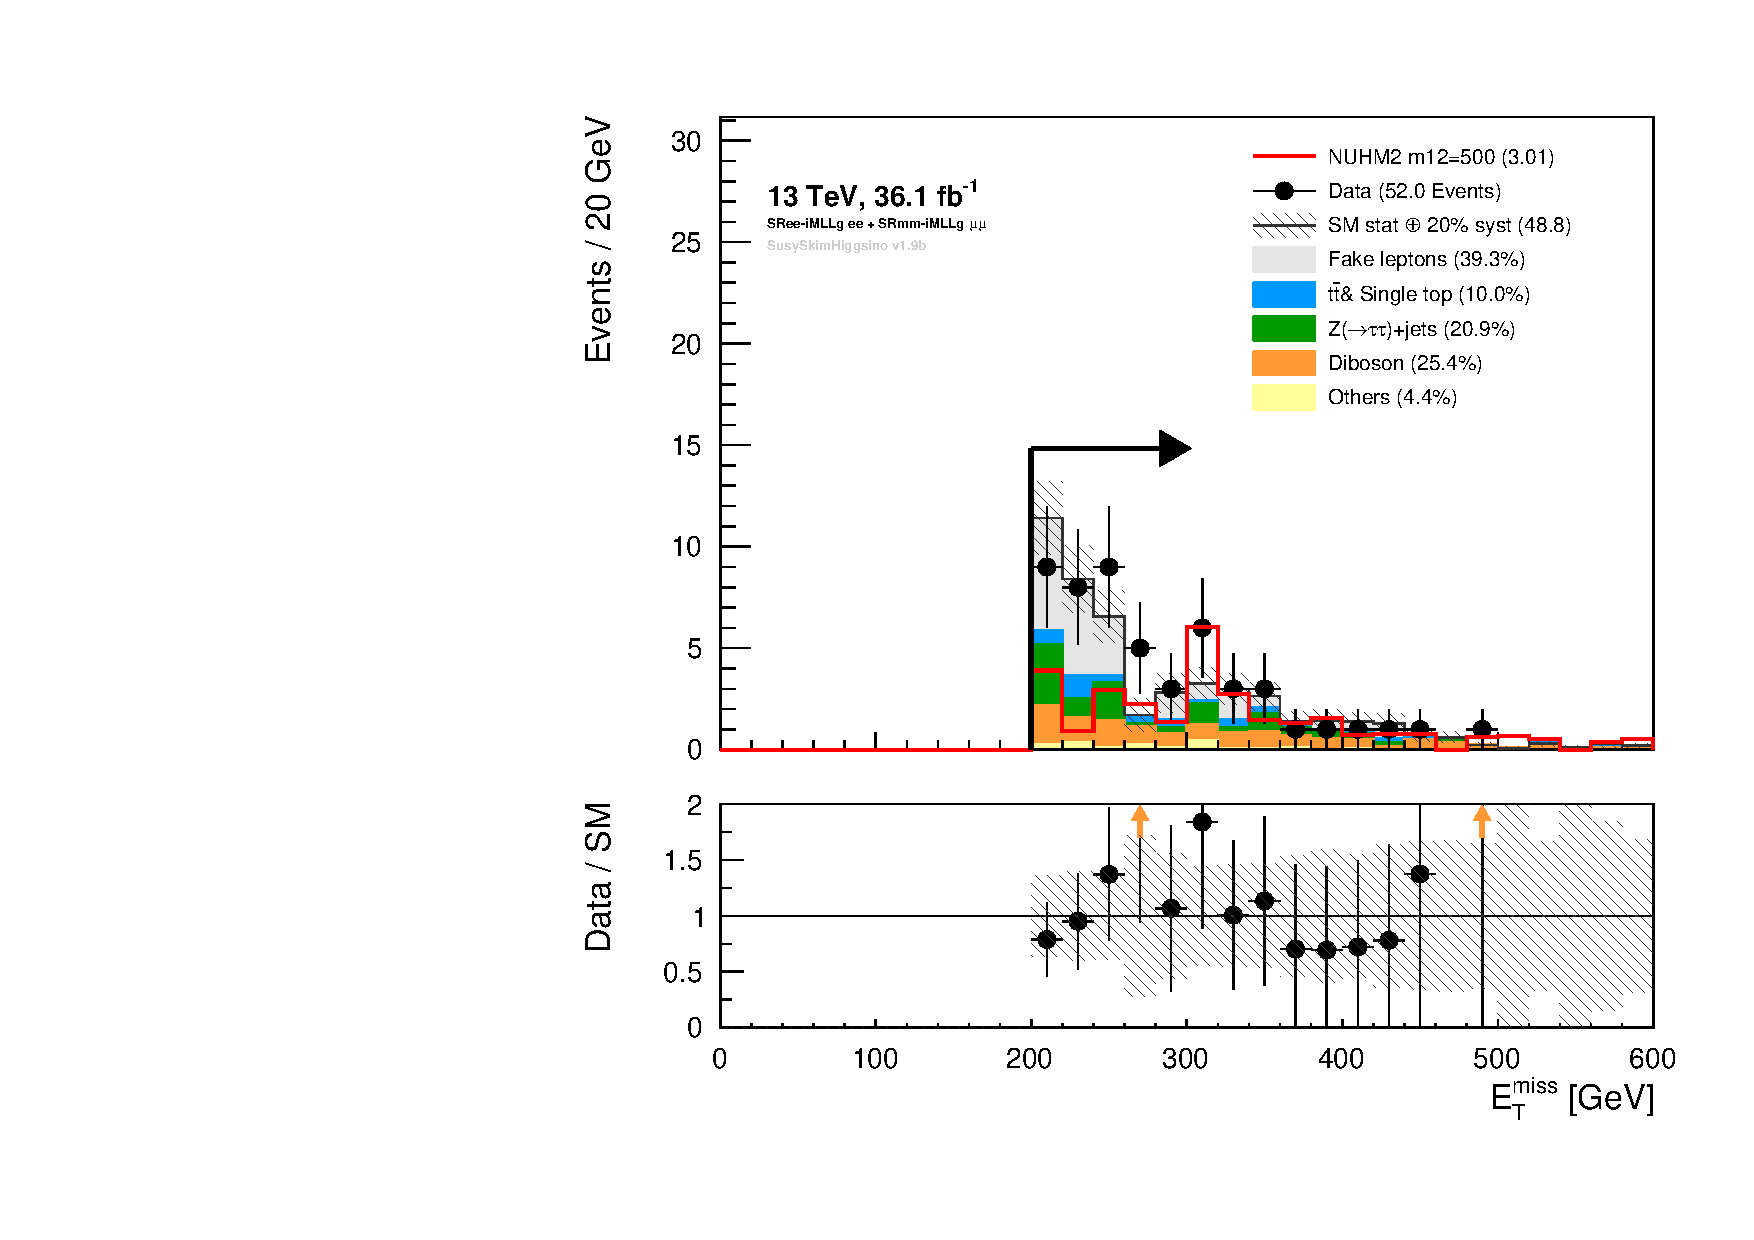
\includegraphics[scale=0.3]{NUHM2_m12_500_and_Bkg_met_Et_SFOS_N_minus_one_distribution_in_SR_times_10_on_Nsig.pdf}
            \caption{$E^{\mathrm{miss}}_{\mathrm{T}}$}
            \label{fig:event_nuhm2_m12_500_met_SFOS}
        \end{subfigure}
        \begin{subfigure}[b]{0.48\textwidth}
            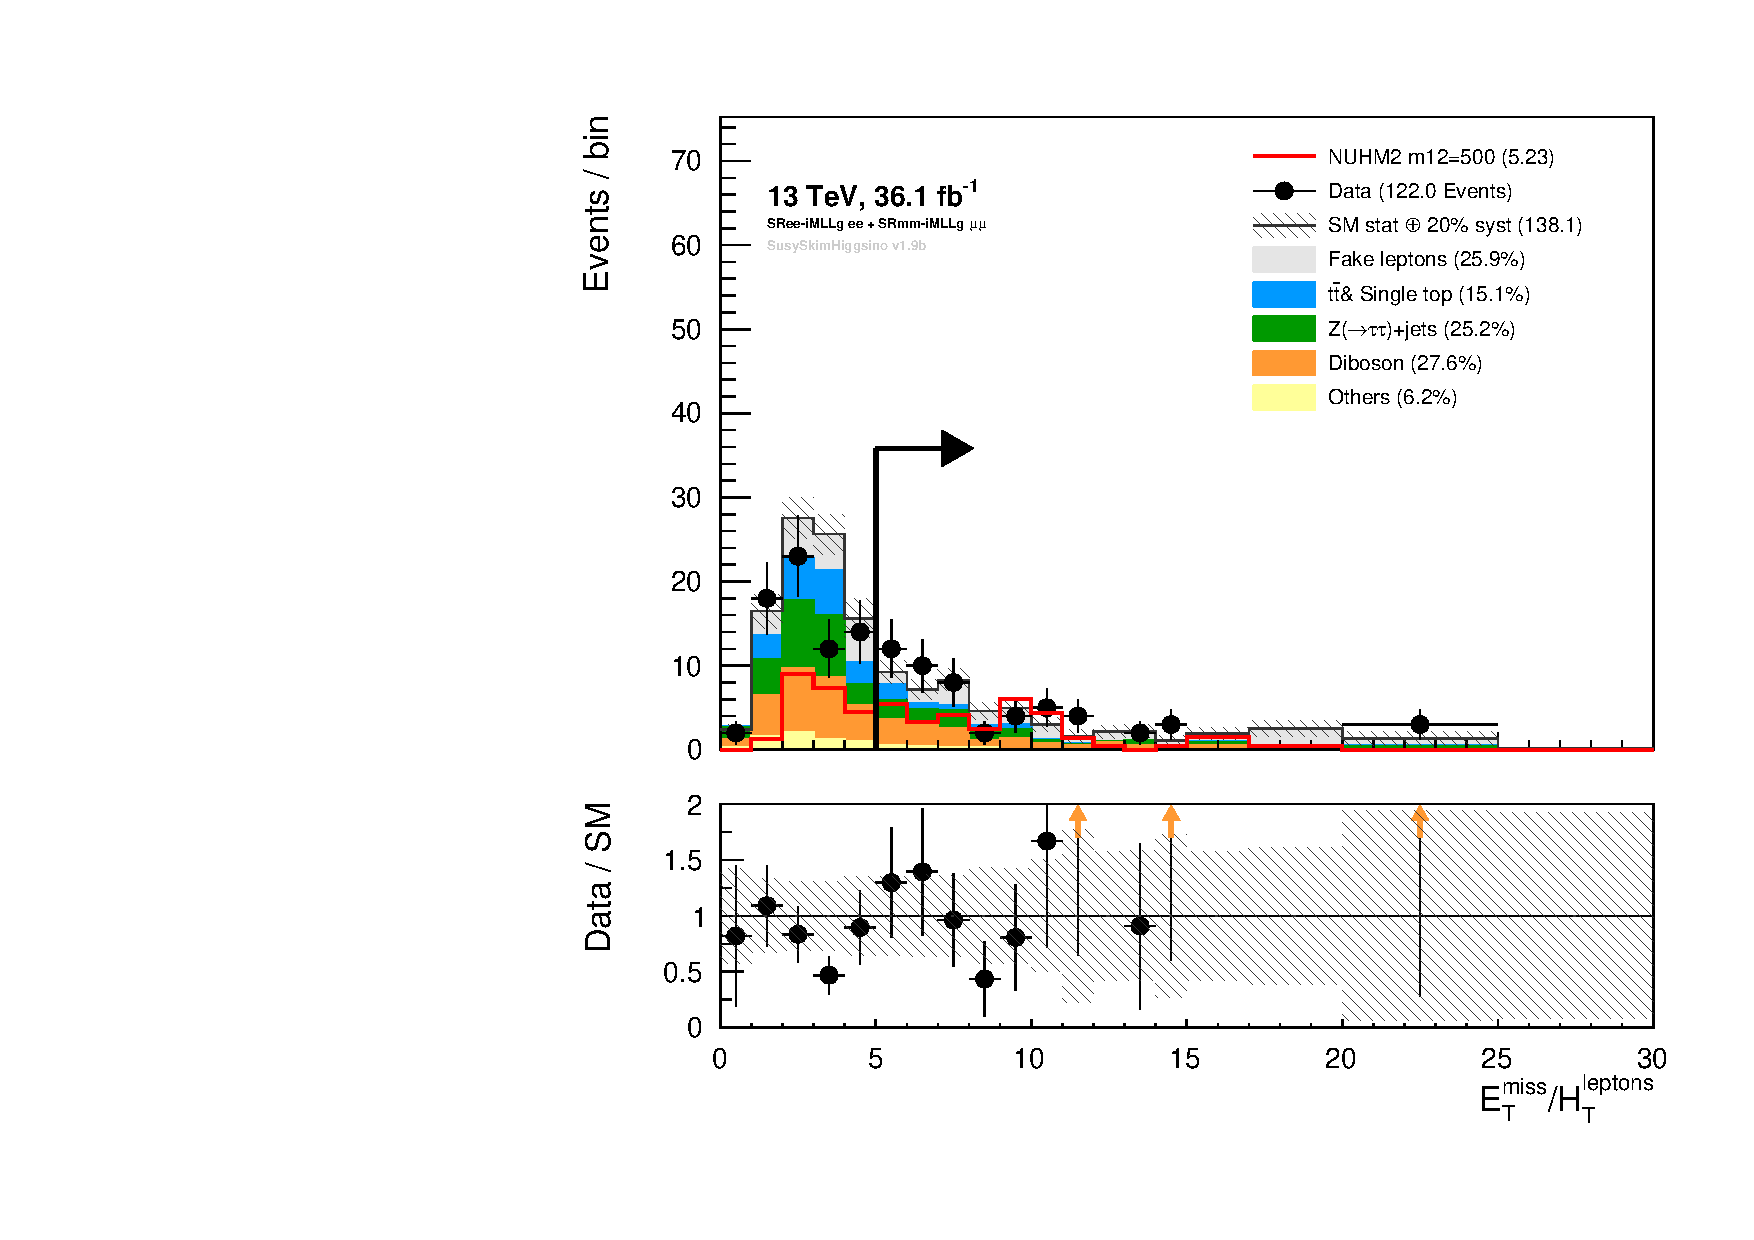
\includegraphics[scale=0.3]{NUHM2_m12_500_and_Bkg_METOverHTLep_SFOS_N_minus_one_distribution_in_SR_times_10_on_Nsig.pdf}
            \caption{$E^{\mathrm{miss}}_{\mathrm{T}} / H^{\mathrm{leptons}}_{\mathrm{T}}$}
            \label{fig:event_nuhm2_m12_500_METOverHTLep_SFOS}
        \end{subfigure}
    \end{center}
    \caption{The `$N-1$' distributions for NUHM2 model with $m_{1/2} = 500$~{\GeV} in SR region $1 < $SR$\ell \ell$-$m_{\ell \ell} < 60$~{\GeV}.
    The NUHM2 distributions are multiplied by 10 but the number of events in the legend use its actual values.}
    \label{fig:event_nuhm2_kinematic_in_SR_SFOS_m12_500_1}
\end{figure}

\begin{figure}[htbp]
    \begin{center}
        \begin{subfigure}[b]{0.48\textwidth}
            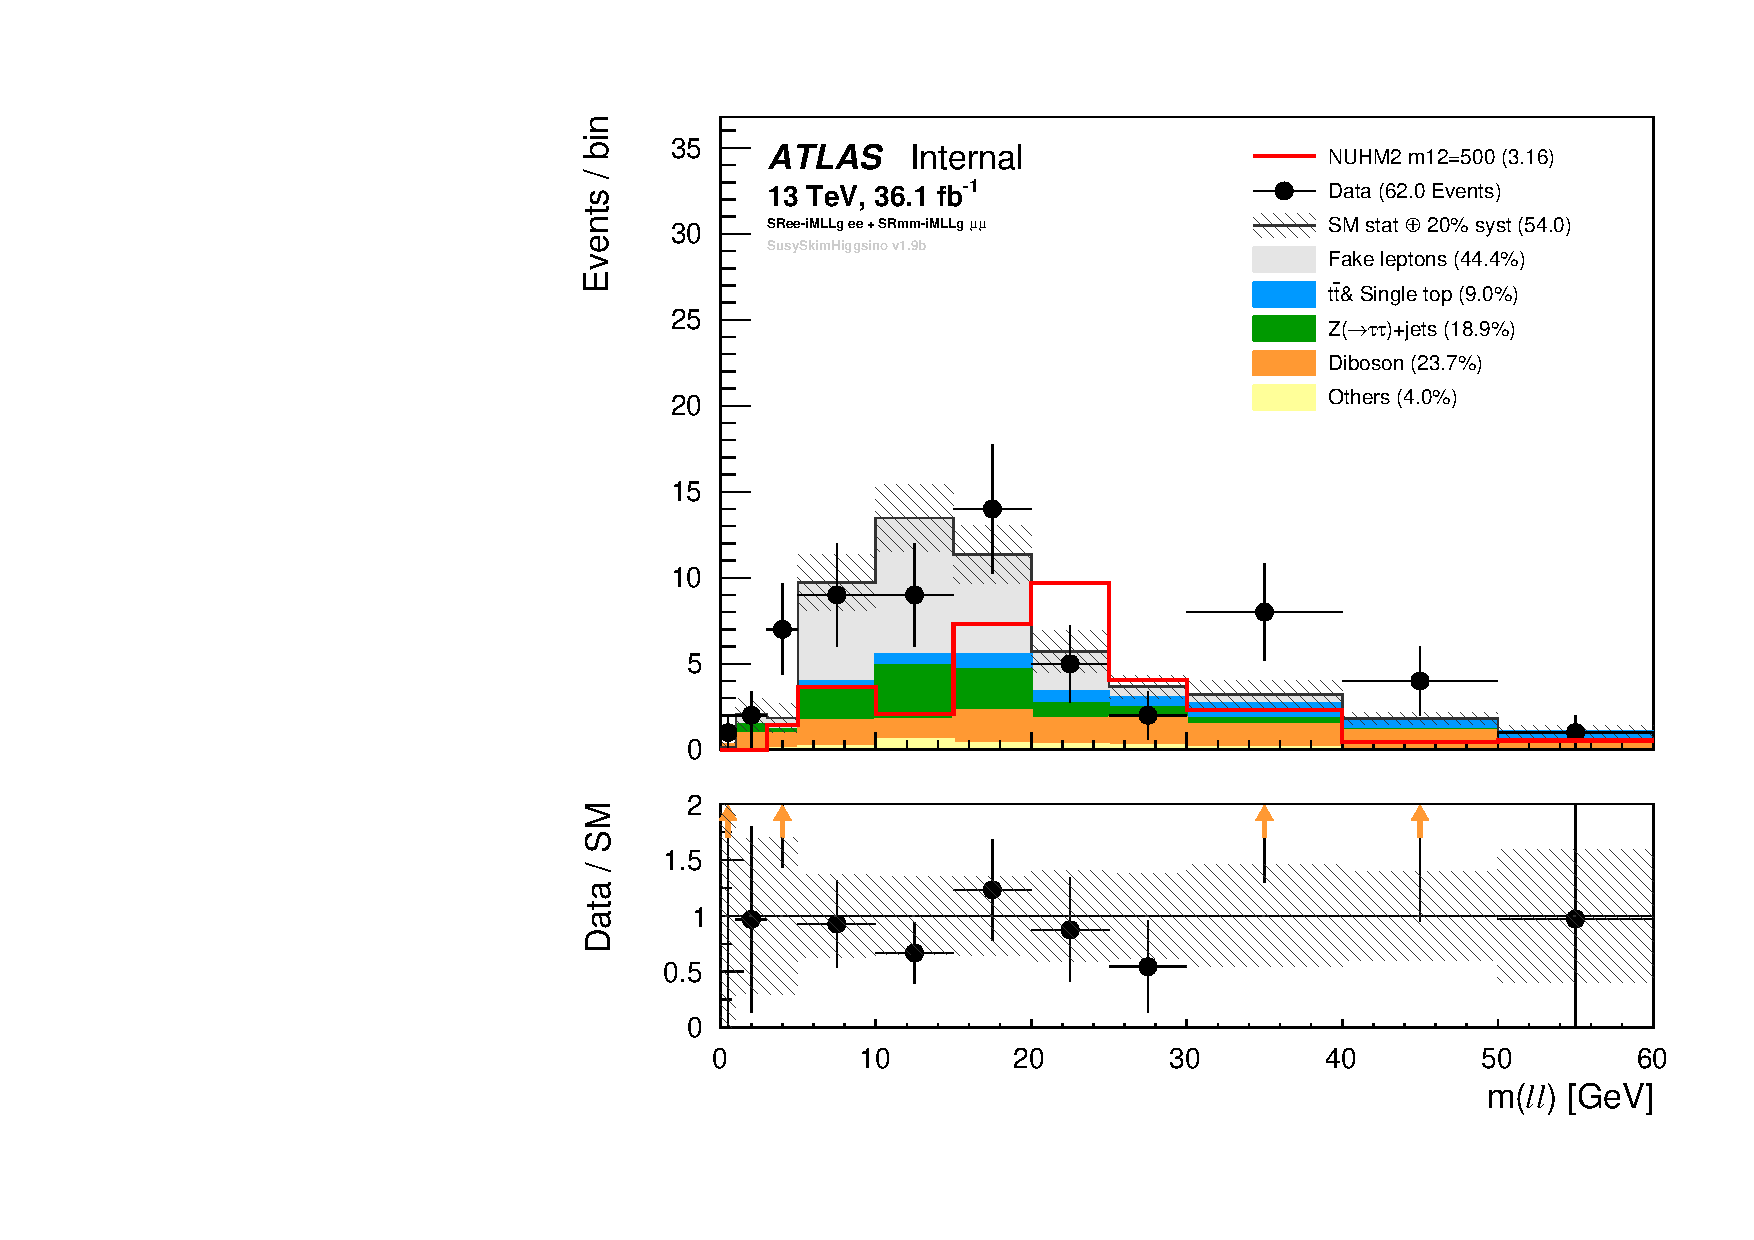
\includegraphics[scale=0.3]{NUHM2_m12_500_and_Bkg_mll_SFOS_N_minus_one_distribution_in_SR_times_10_on_Nsig.pdf}
            \caption{$m_{\ell\ell}$}
            \label{fig:event_nuhm2_m12_500_mll_SFOS}
        \end{subfigure}
        \begin{subfigure}[b]{0.48\textwidth}
            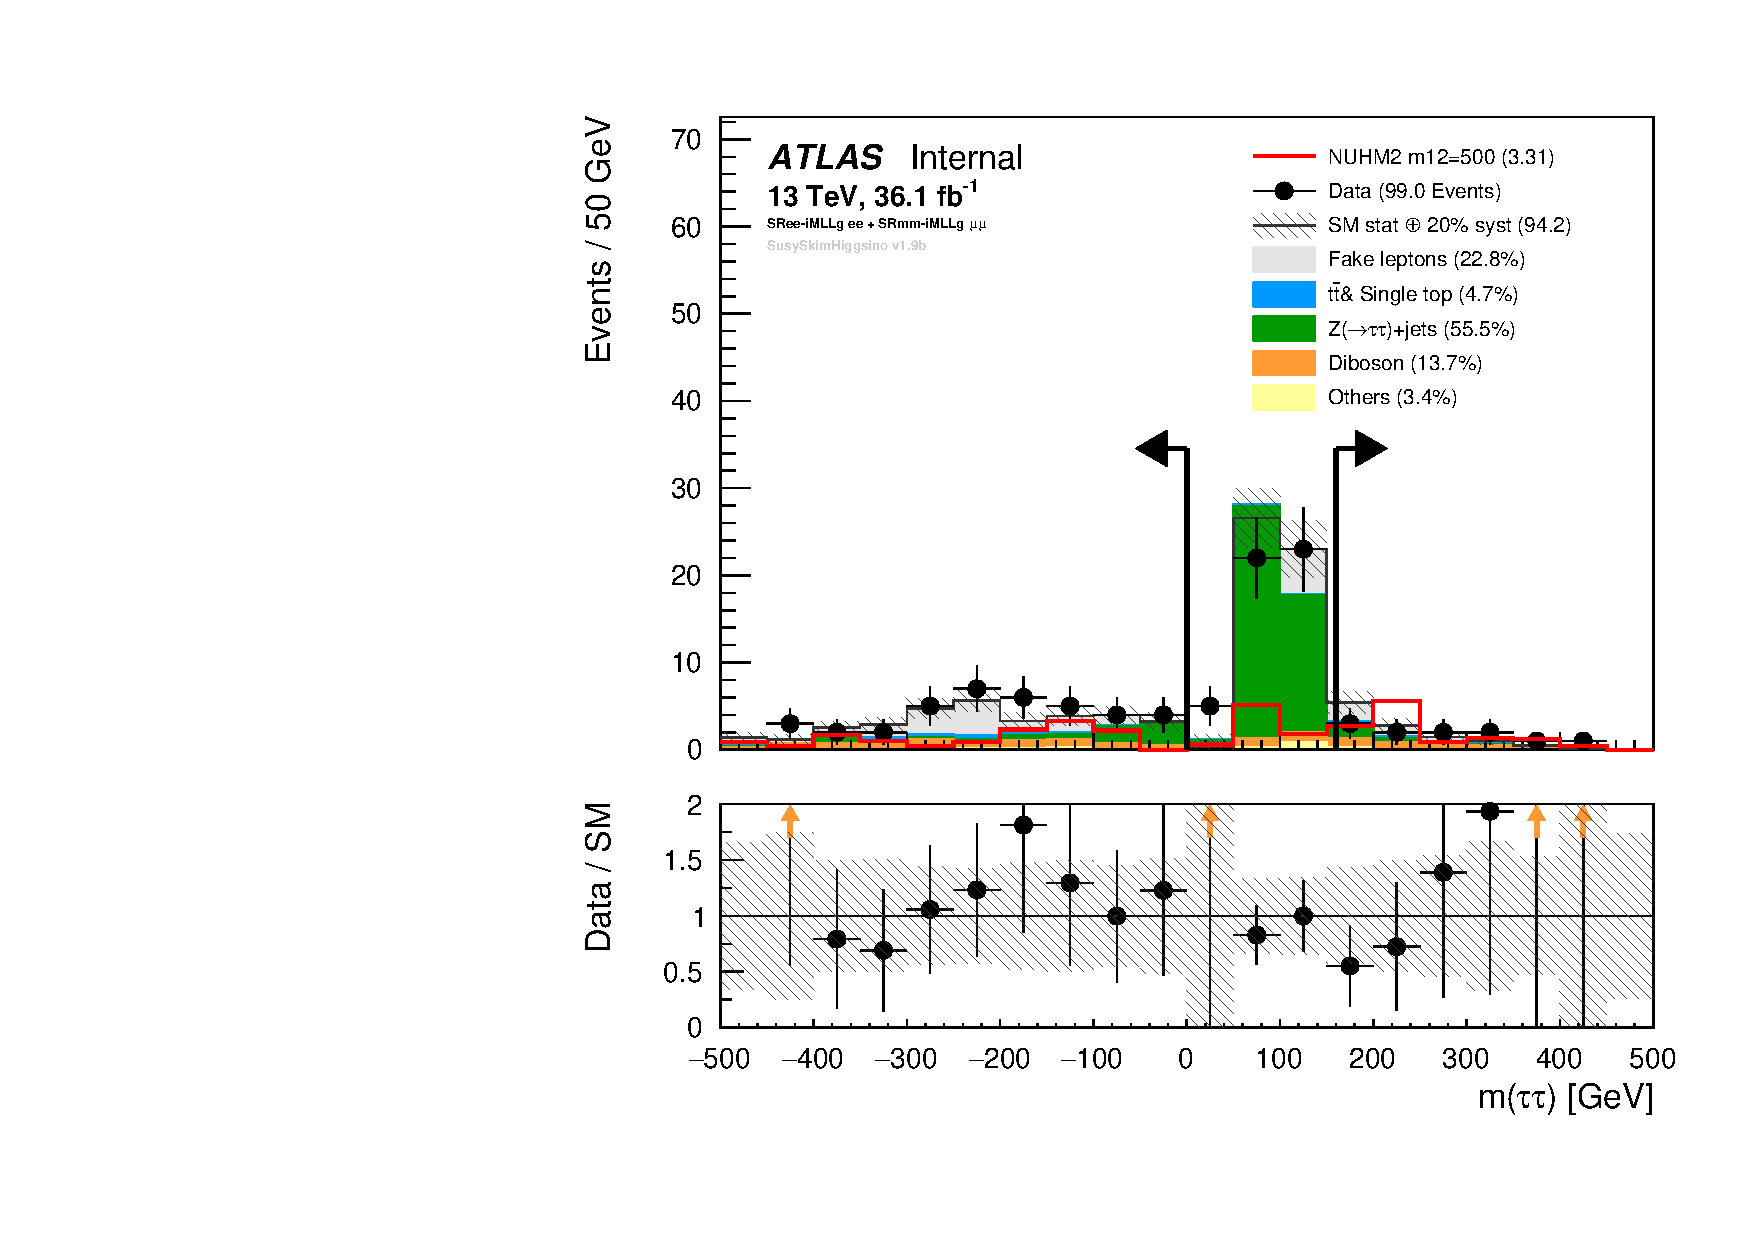
\includegraphics[scale=0.3]{NUHM2_m12_500_and_Bkg_MTauTau_SFOS_N_minus_one_distribution_in_SR_times_10_on_Nsig.pdf}
            \caption{$m_{\tau\tau}$}
            \label{fig:event_nuhm2_m12_500_MTauTau_SFOS}
        \end{subfigure}
        \begin{subfigure}[b]{0.48\textwidth}
            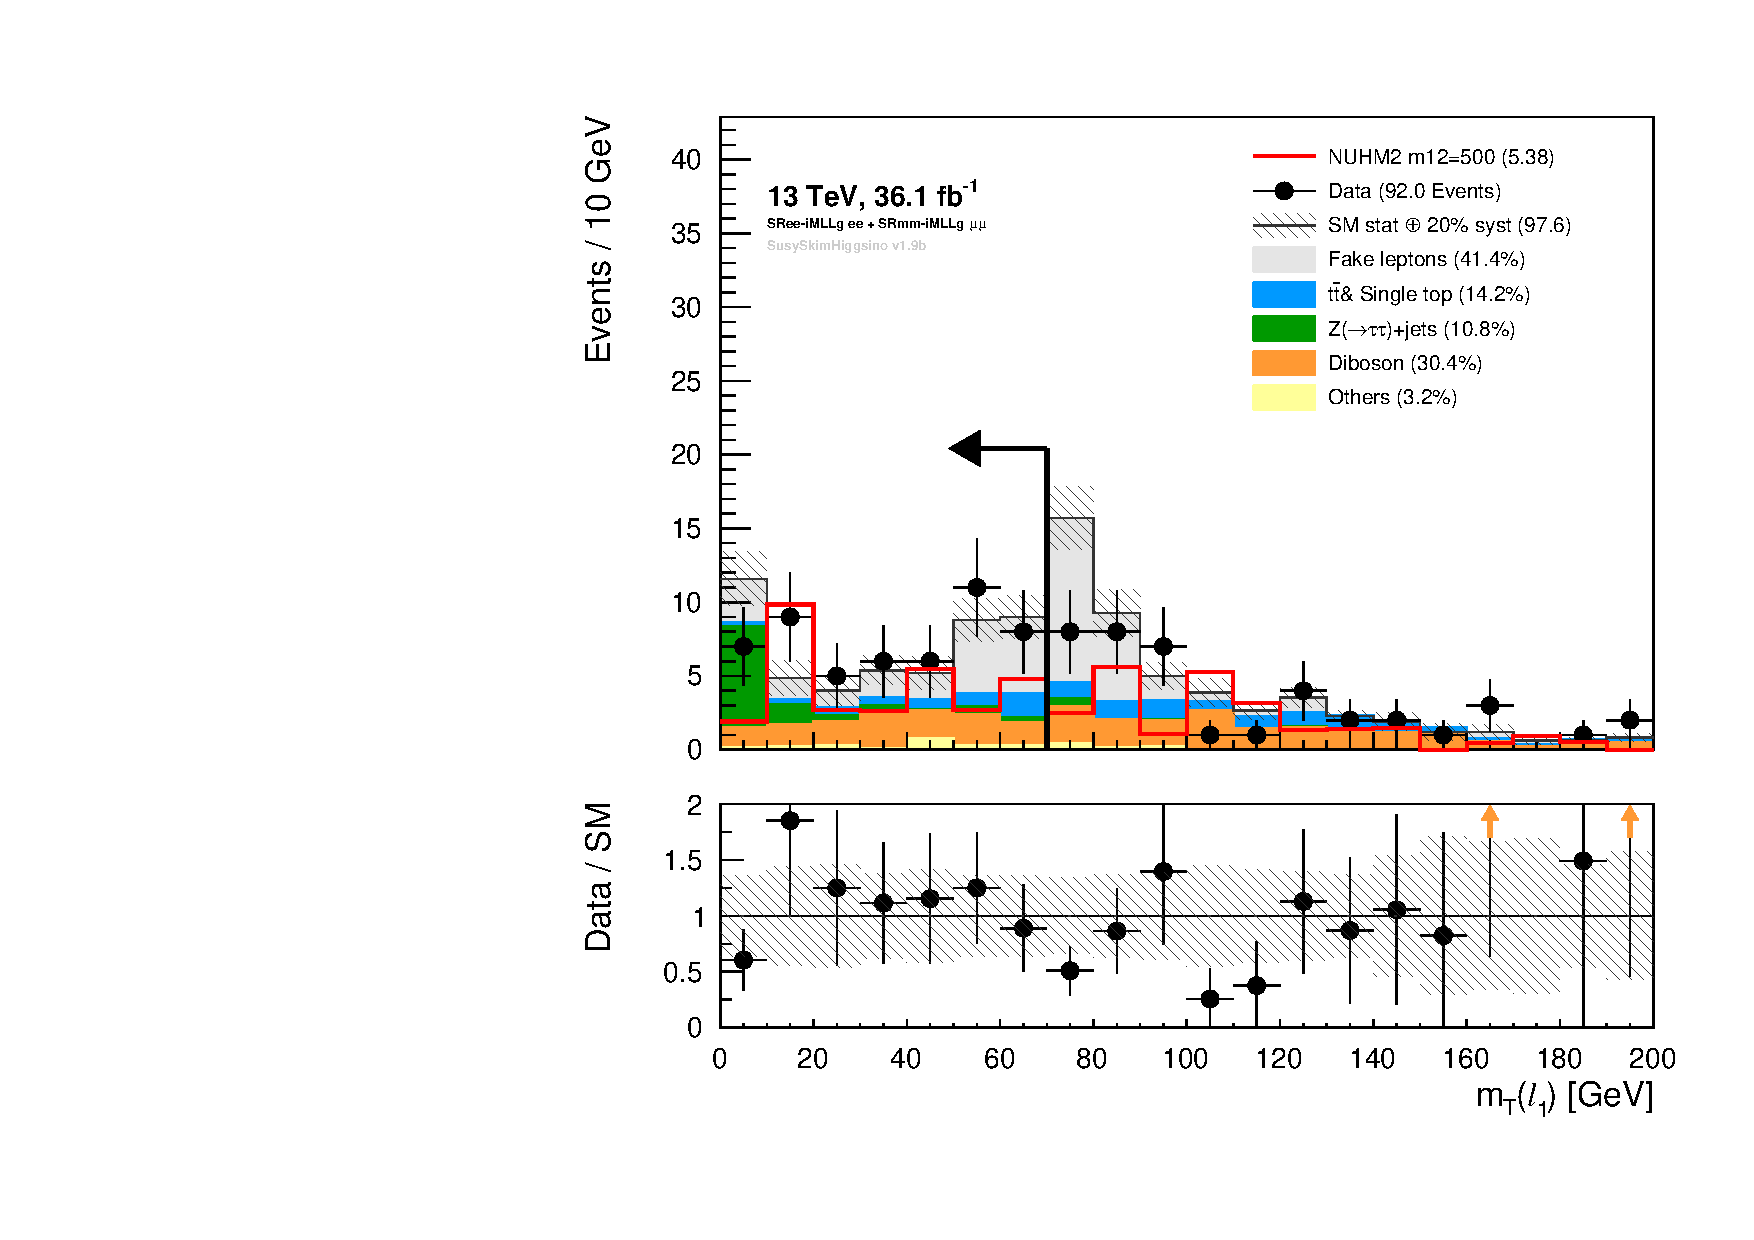
\includegraphics[scale=0.3]{NUHM2_m12_500_and_Bkg_mt_lep1_SFOS_N_minus_one_distribution_in_SR_times_10_on_Nsig.pdf}
            \caption{$m_{T}(\ell_{1})$}
            \label{fig:event_nuhm2_m12_500_mt_lep1_SFOS}
        \end{subfigure}
        \begin{subfigure}[b]{0.48\textwidth}
            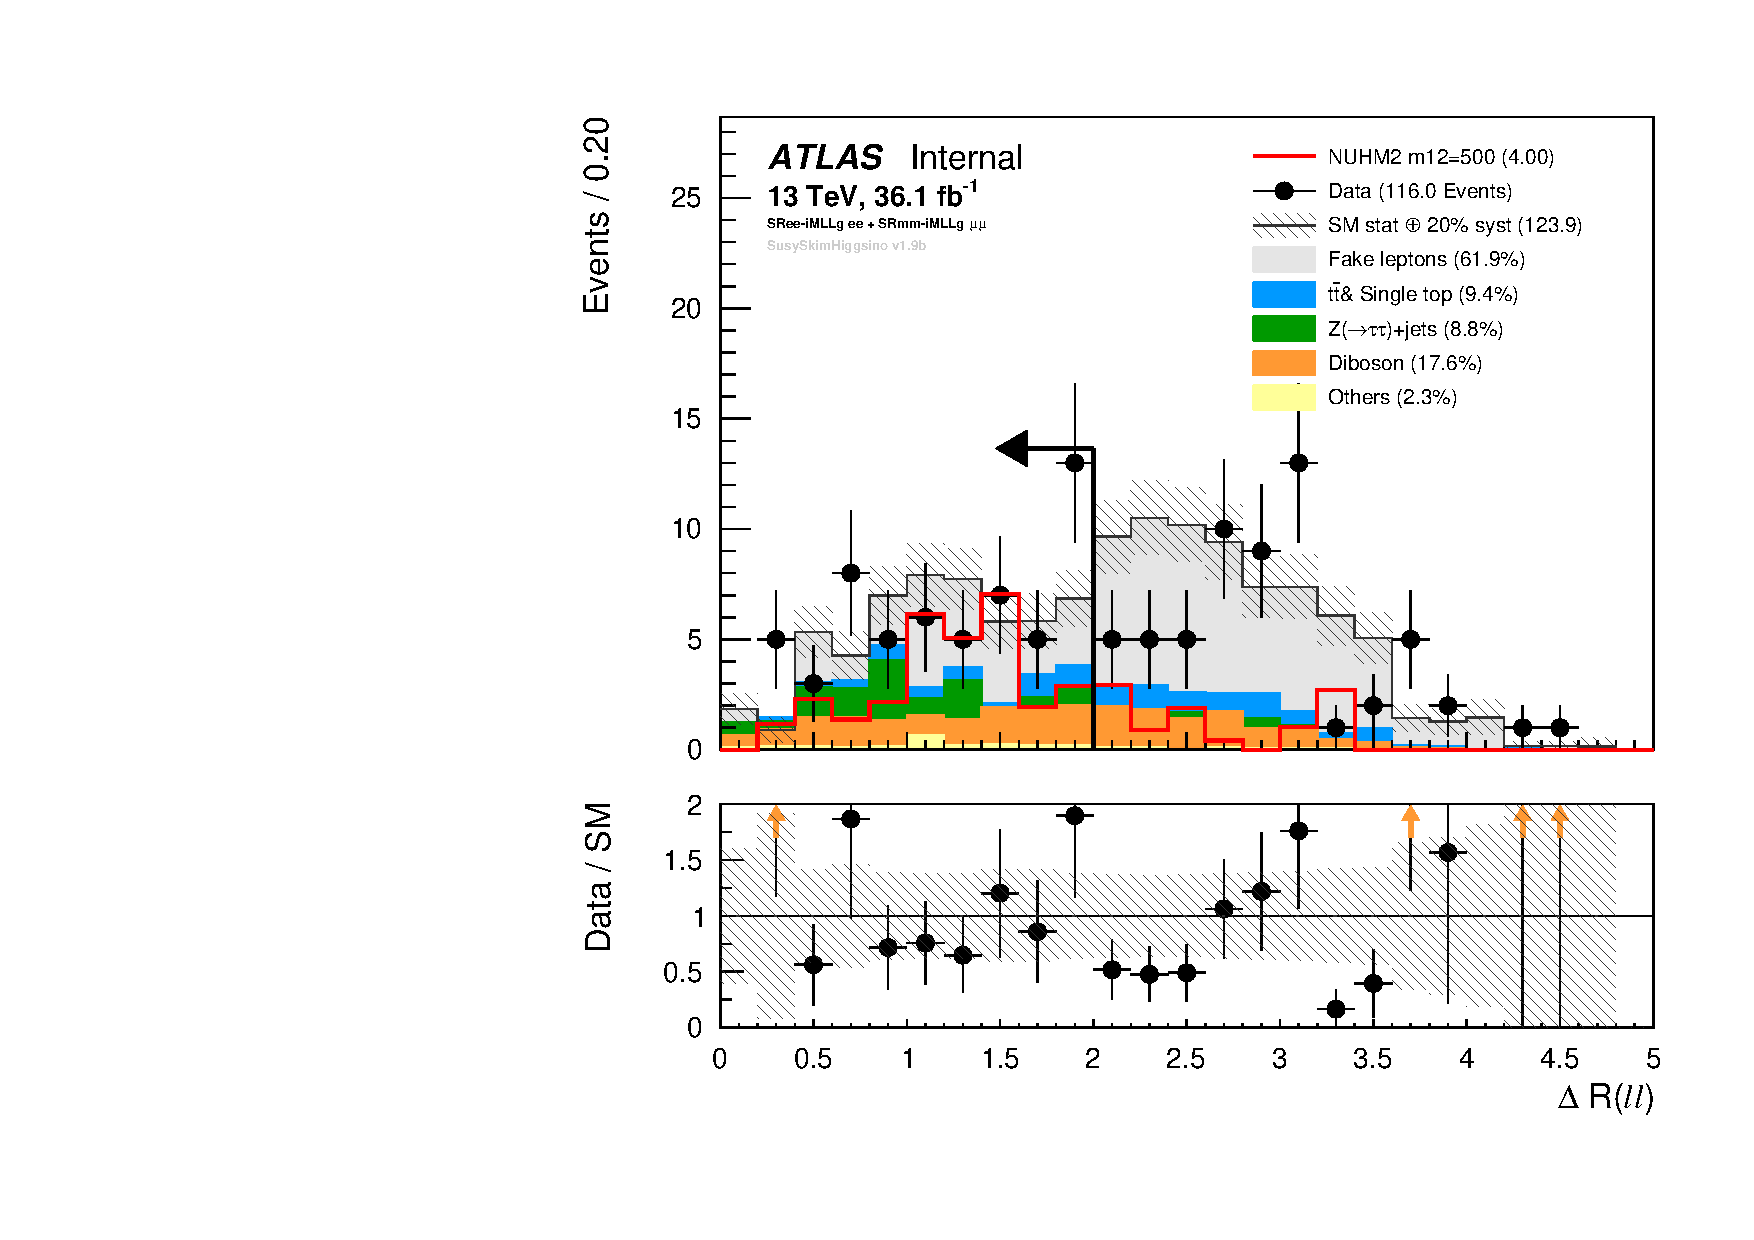
\includegraphics[scale=0.3]{NUHM2_m12_500_and_Bkg_Rll_SFOS_N_minus_one_distribution_in_SR_times_10_on_Nsig.pdf}
            \caption{$\Delta R_{\ell\ell}$}
            \label{fig:event_nuhm2_m12_500_Rll_SFOS}
        \end{subfigure}
        \begin{subfigure}[b]{0.48\textwidth}
            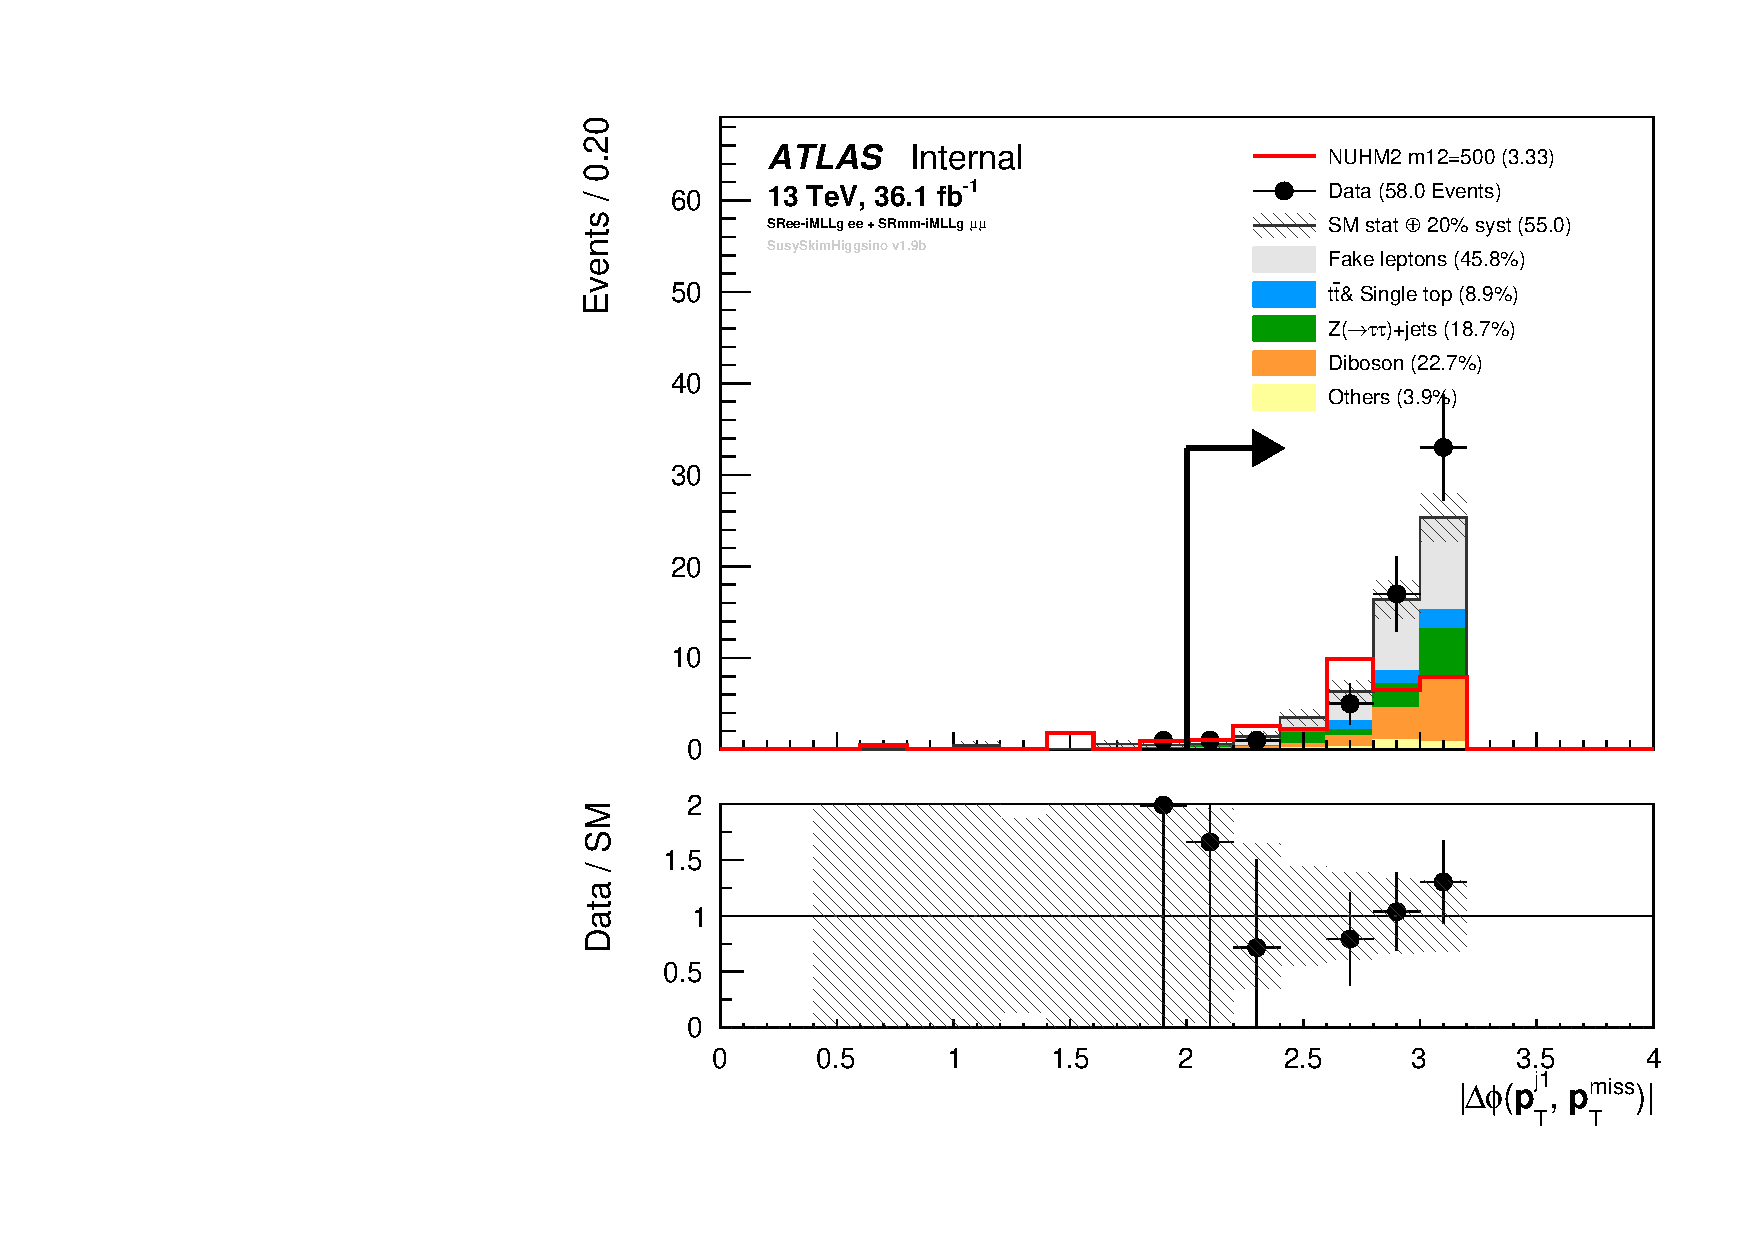
\includegraphics[scale=0.3]{NUHM2_m12_500_and_Bkg_DPhiJ1Met_SFOS_N_minus_one_distribution_in_SR_times_10_on_Nsig.pdf}
            \caption{$|\Delta \phi(\mathbf{p}^{j_{1}}_{\mathrm{T}}, \mathbf{p}^{\mathrm{miss}}_{\mathrm{T}})|$}
            \label{fig:event_nuhm2_m12_500_DPhiJ1Met_SFOS}
        \end{subfigure}
        \begin{subfigure}[b]{0.48\textwidth}
            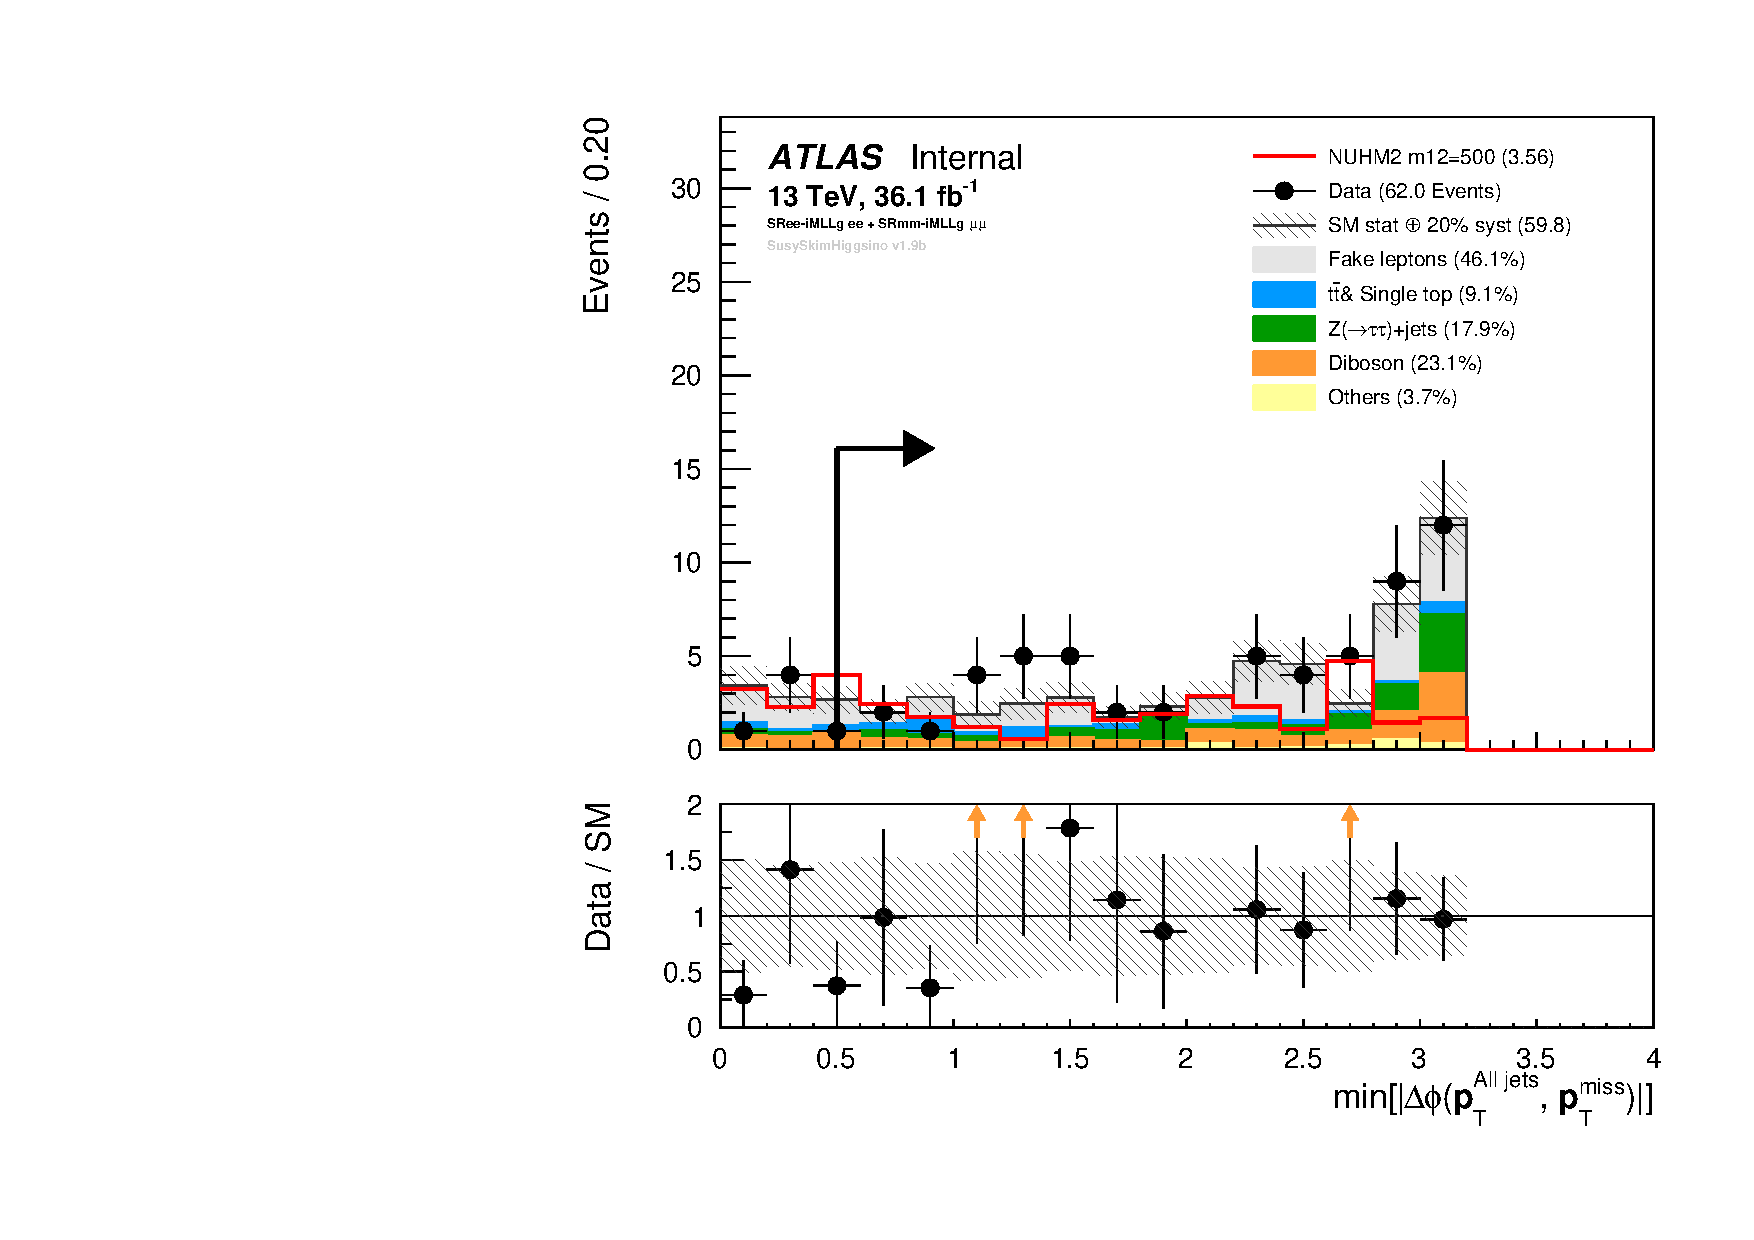
\includegraphics[scale=0.3]{NUHM2_m12_500_and_Bkg_minDPhiAllJetsMet_SFOS_N_minus_one_distribution_in_SR_times_10_on_Nsig.pdf}
            \caption{min[$|\Delta \phi(\mathbf{p}^{\textrm{All jets}}_{\mathrm{T}}, \mathbf{p}^{\mathrm{miss}}_{\mathrm{T}})|$]}
            \label{fig:event_nuhm2_m12_500_minDPhiAllJetsMet_SFOS}
        \end{subfigure}
    \end{center}
    \caption{The `$N-1$' distributions for NUHM2 model with $m_{1/2} = 500$~{\GeV} in SR region $1 < $SR$\ell \ell$-$m_{\ell \ell} < 60$~{\GeV}.
    The NUHM2 distributions are multiplied by 10 but the number of events in the legend use its actual values.}
    \label{fig:event_nuhm2_kinematic_in_SR_SFOS_m12_500_2}
\end{figure}

% m12 = 600
\begin{figure}[htbp]
    \begin{center}
        \begin{subfigure}[b]{0.48\textwidth}
            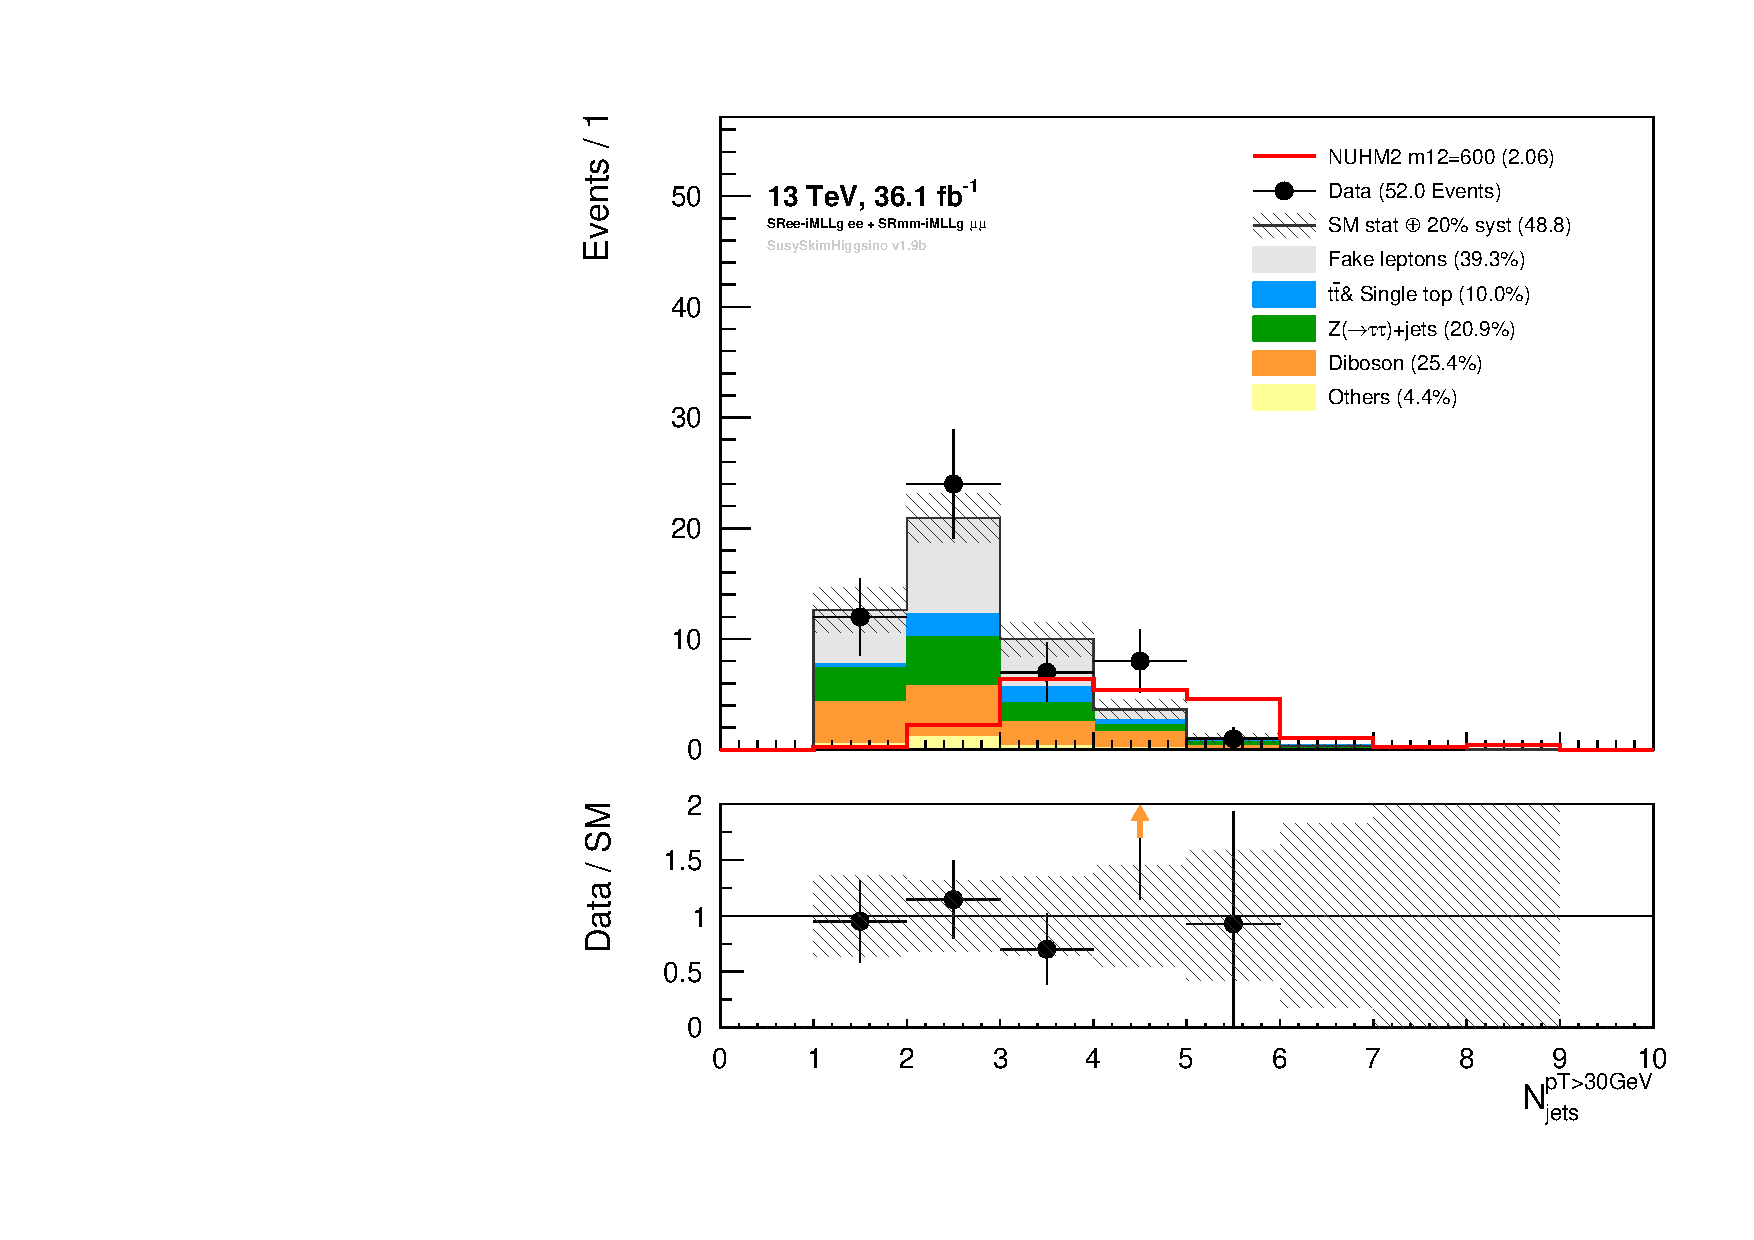
\includegraphics[scale=0.3]{NUHM2_m12_600_and_Bkg_nJet30_SFOS_N_minus_one_distribution_in_SR_times_10_on_Nsig.pdf}
            \caption{$N^{30}_{\mathrm{jets}}$}
            \label{fig:event_nuhm2_m12_600_nJet30_SFOS}
        \end{subfigure}
        \begin{subfigure}[b]{0.48\textwidth}
            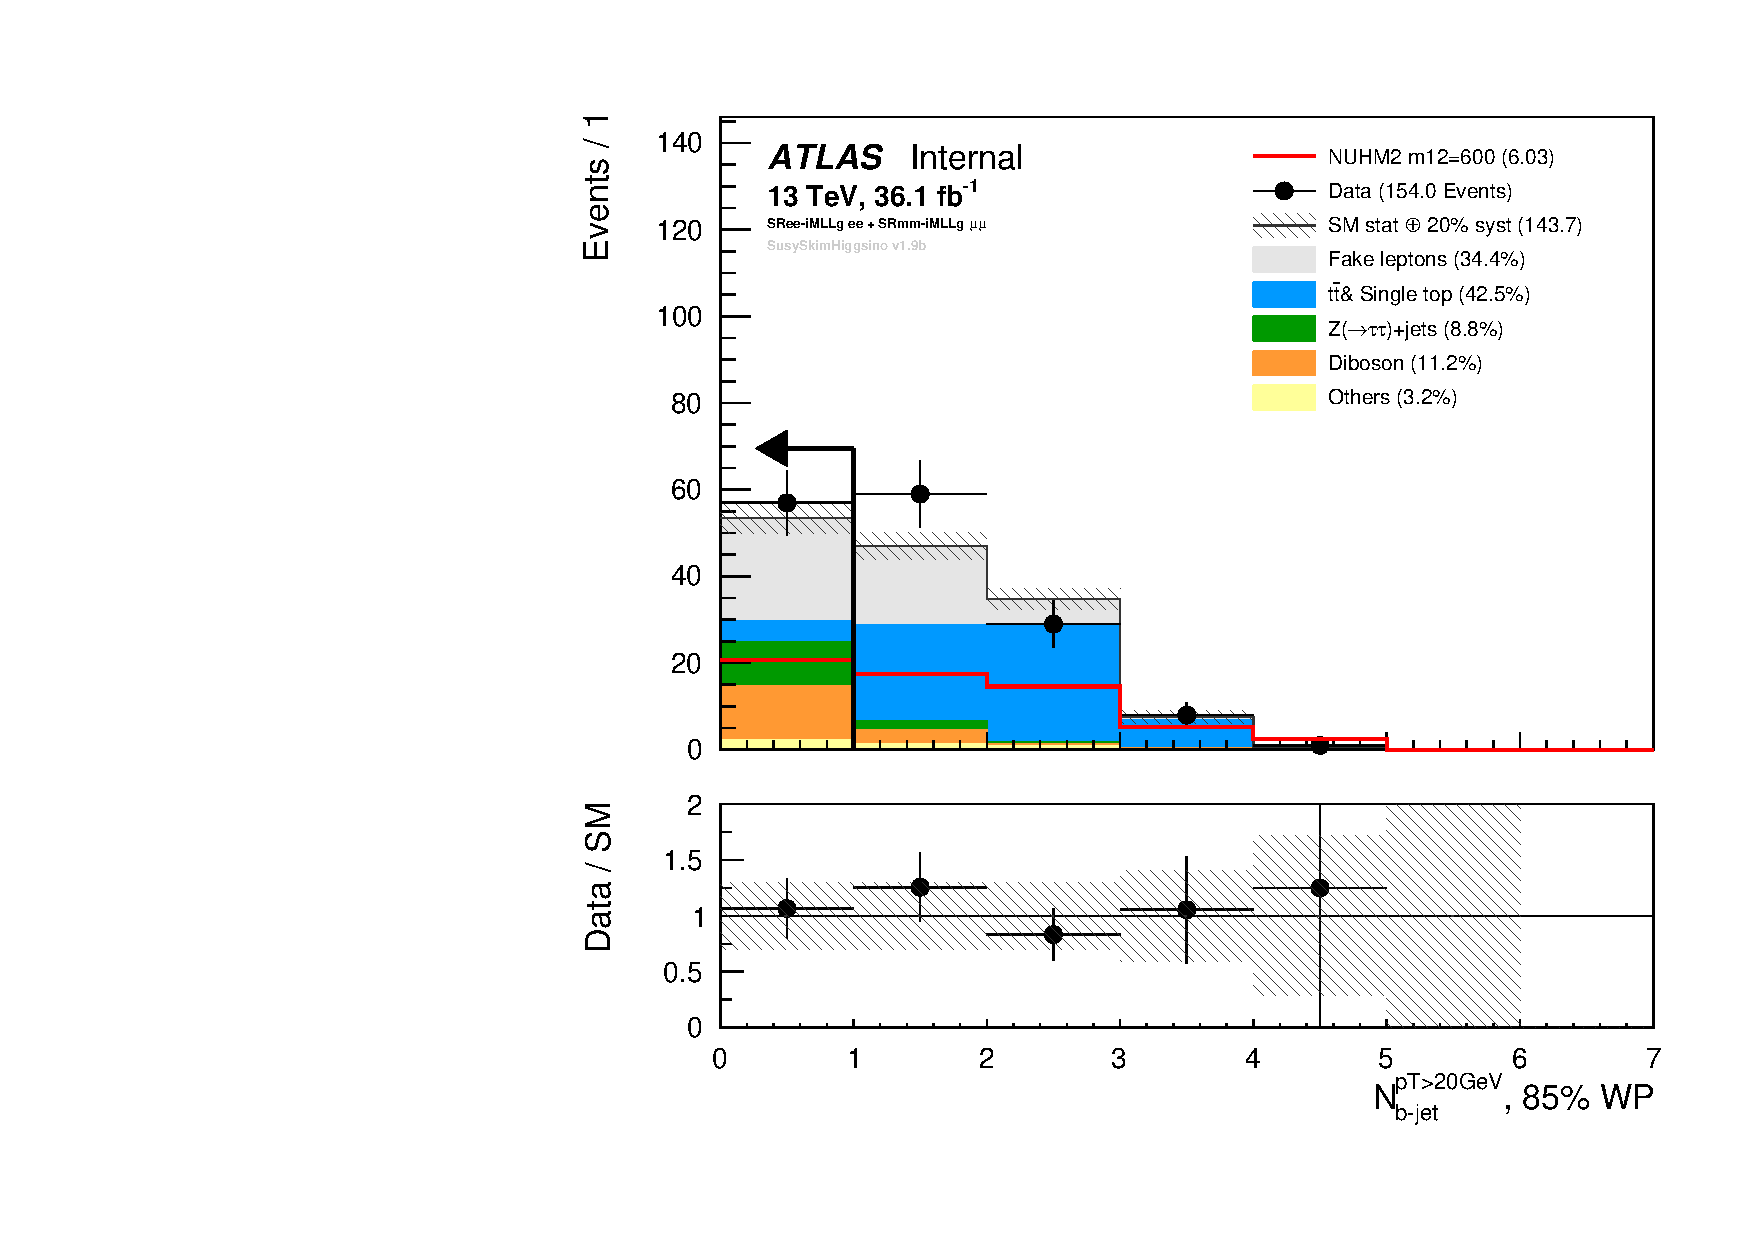
\includegraphics[scale=0.3]{NUHM2_m12_600_and_Bkg_nBJet20_MV2c10_SFOS_N_minus_one_distribution_in_SR_times_10_on_Nsig.pdf}
            \caption{$N^{20}_{\mathrm{b-jets}}$}
            \label{fig:event_nuhm2_m12_600_nBJet20_SFOS}
        \end{subfigure}
        \begin{subfigure}[b]{0.48\textwidth}
            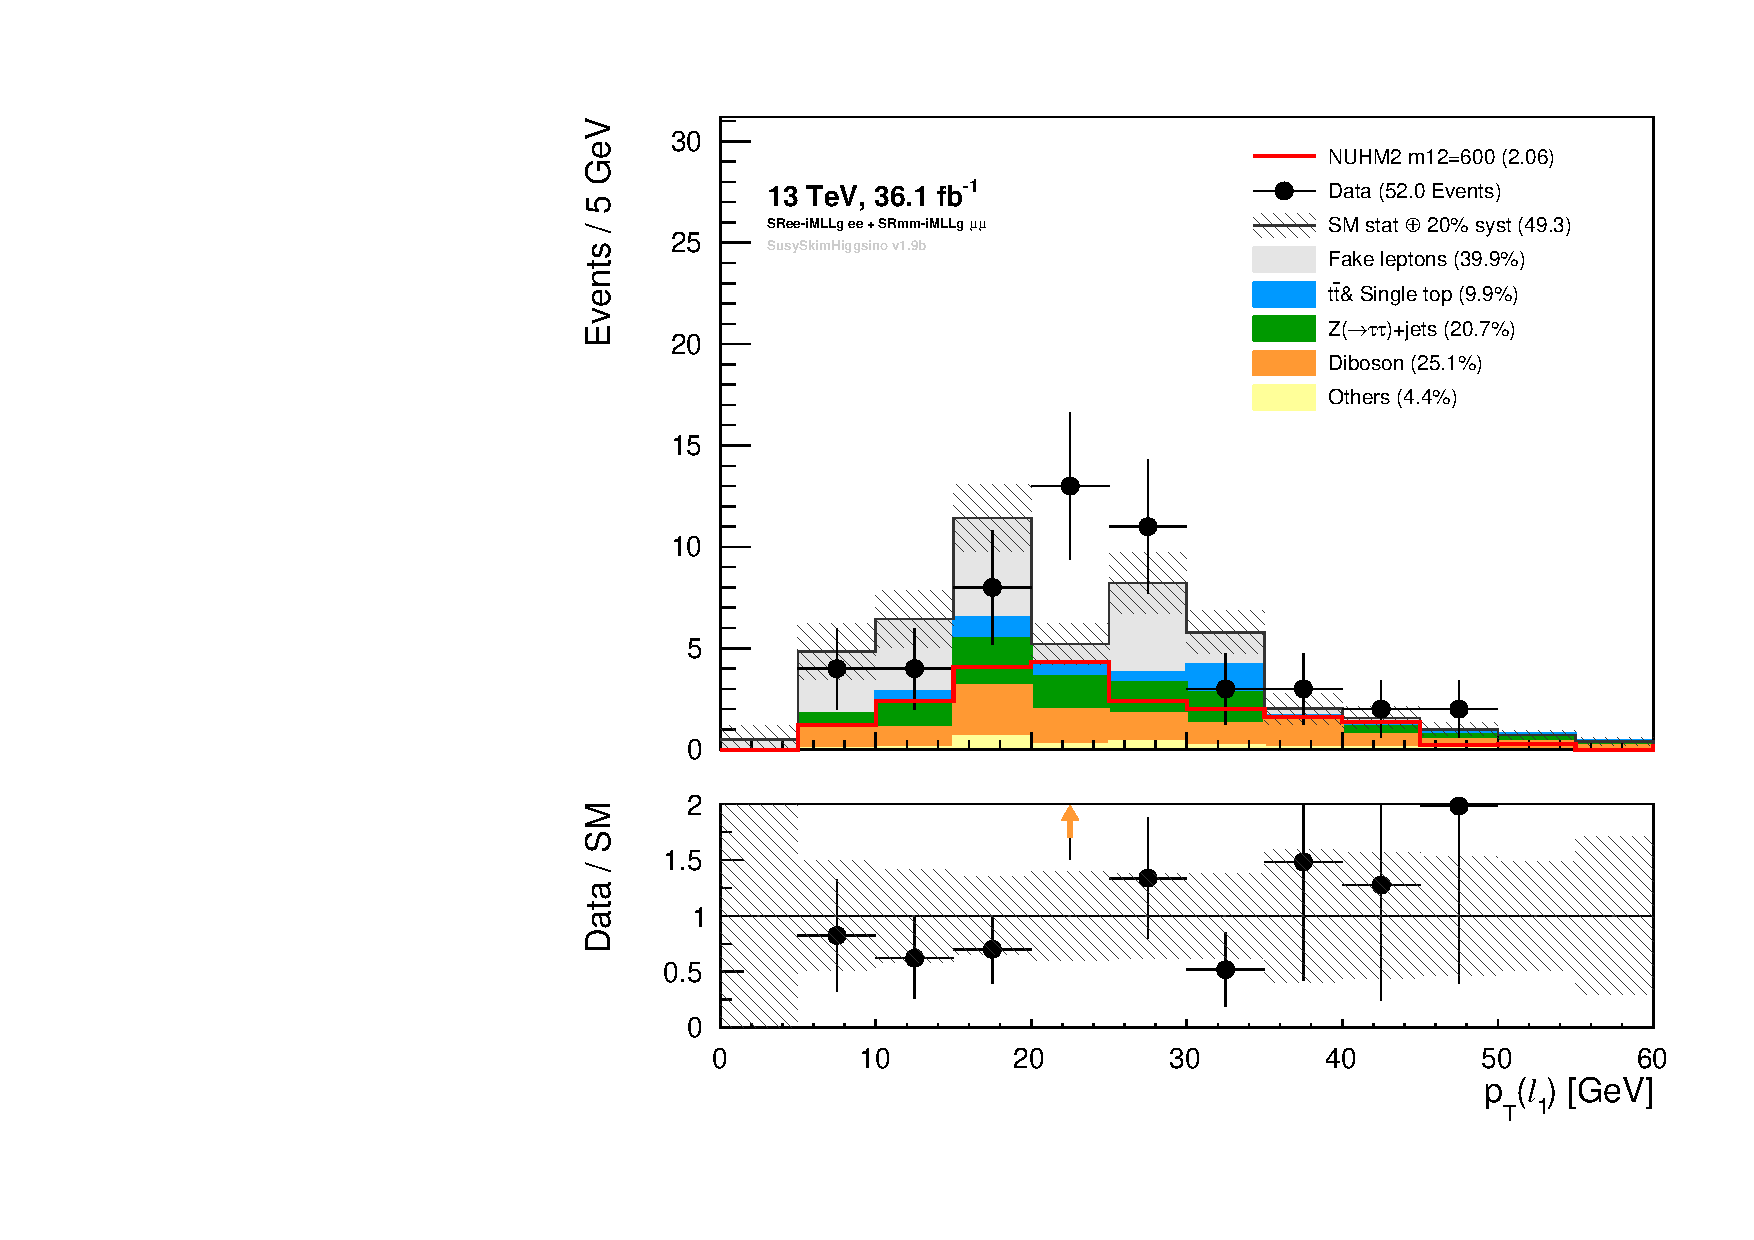
\includegraphics[scale=0.3]{NUHM2_m12_600_and_Bkg_lep1Pt_SFOS_N_minus_one_distribution_in_SR_times_10_on_Nsig.pdf}
            \caption{$p^{\ell_1}_{\mathrm{T}}$}
            \label{fig:event_nuhm2_m12_600_lep1Pt_SFOS}
        \end{subfigure}
        \begin{subfigure}[b]{0.48\textwidth}
            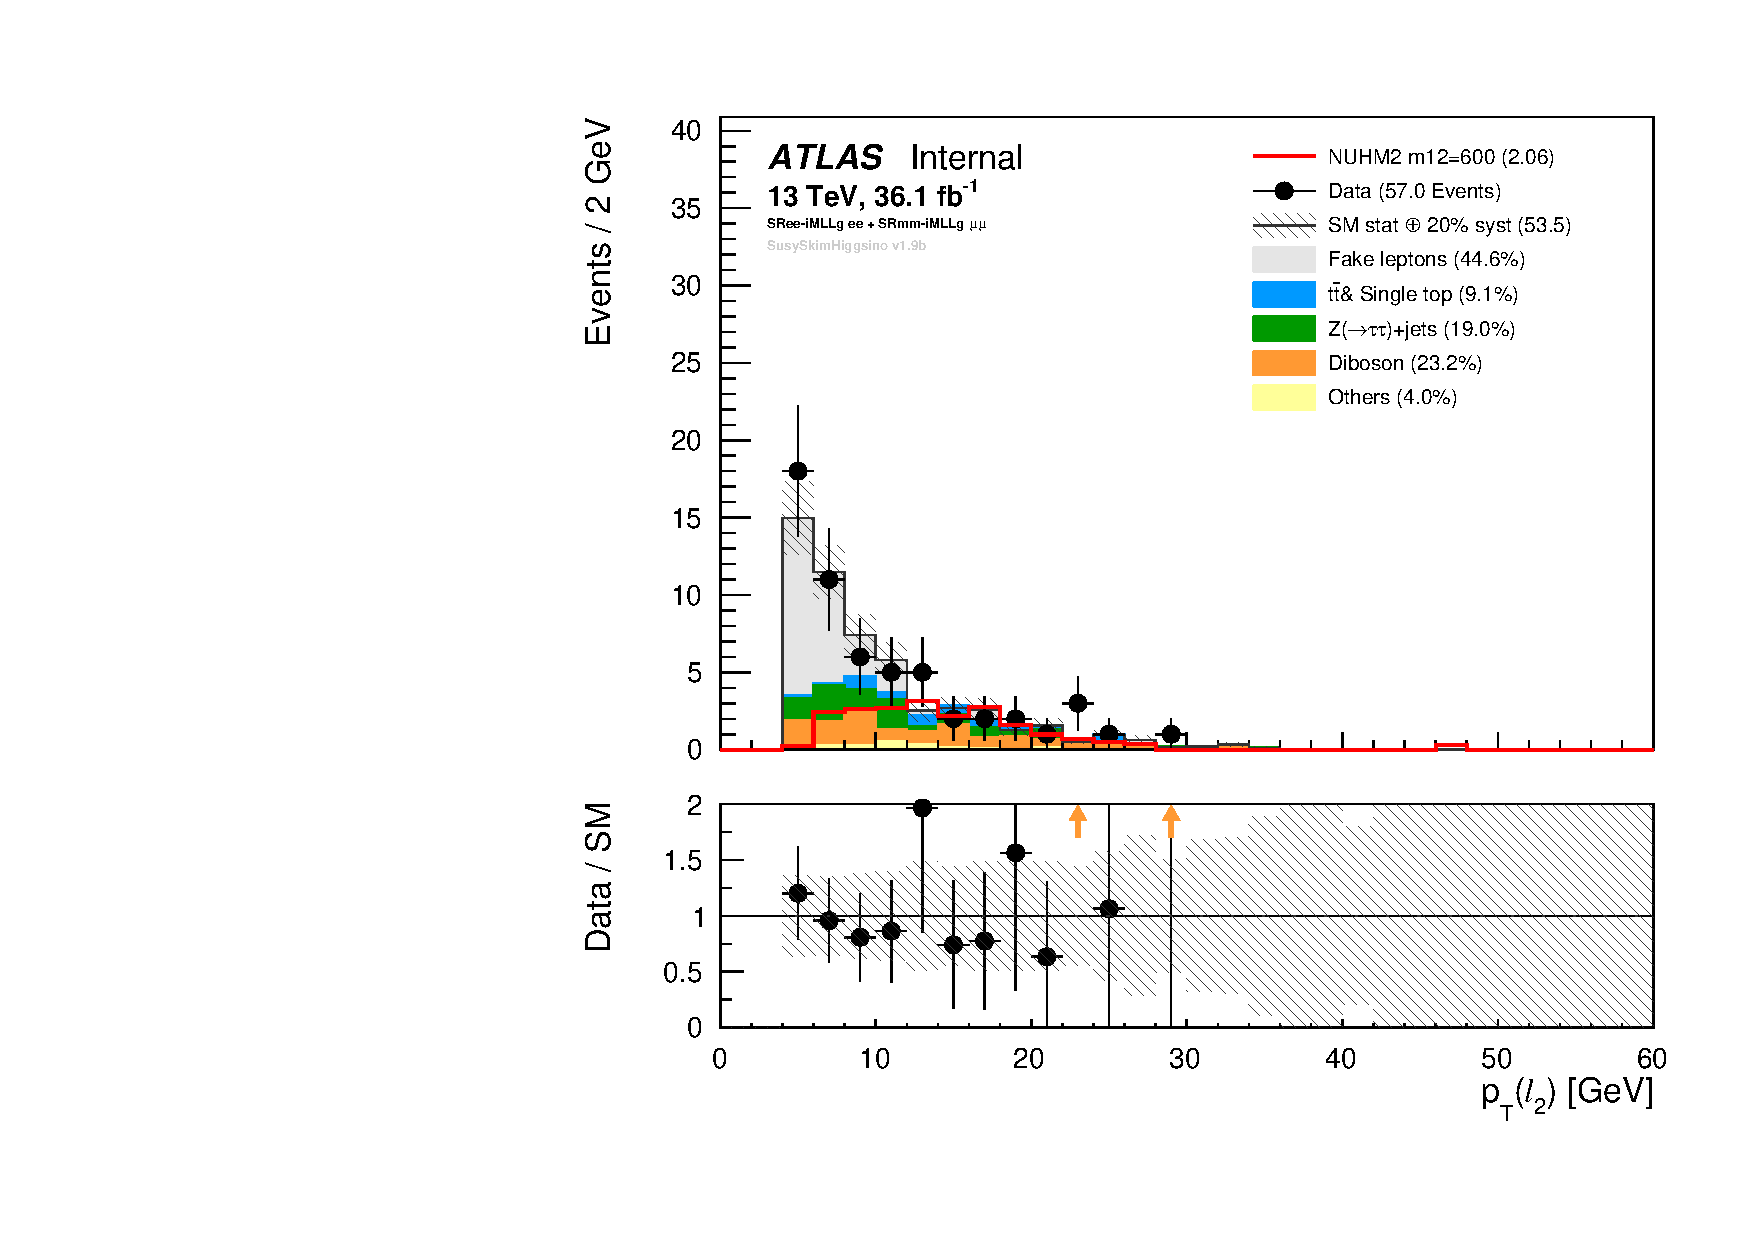
\includegraphics[scale=0.3]{NUHM2_m12_600_and_Bkg_lep2Pt_SFOS_N_minus_one_distribution_in_SR_times_10_on_Nsig.pdf}
            \caption{$p^{\ell_2}_{\mathrm{T}}$}
            \label{fig:event_nuhm2_m12_600_lep2Pt_SFOS}
        \end{subfigure}
        \begin{subfigure}[b]{0.48\textwidth}
            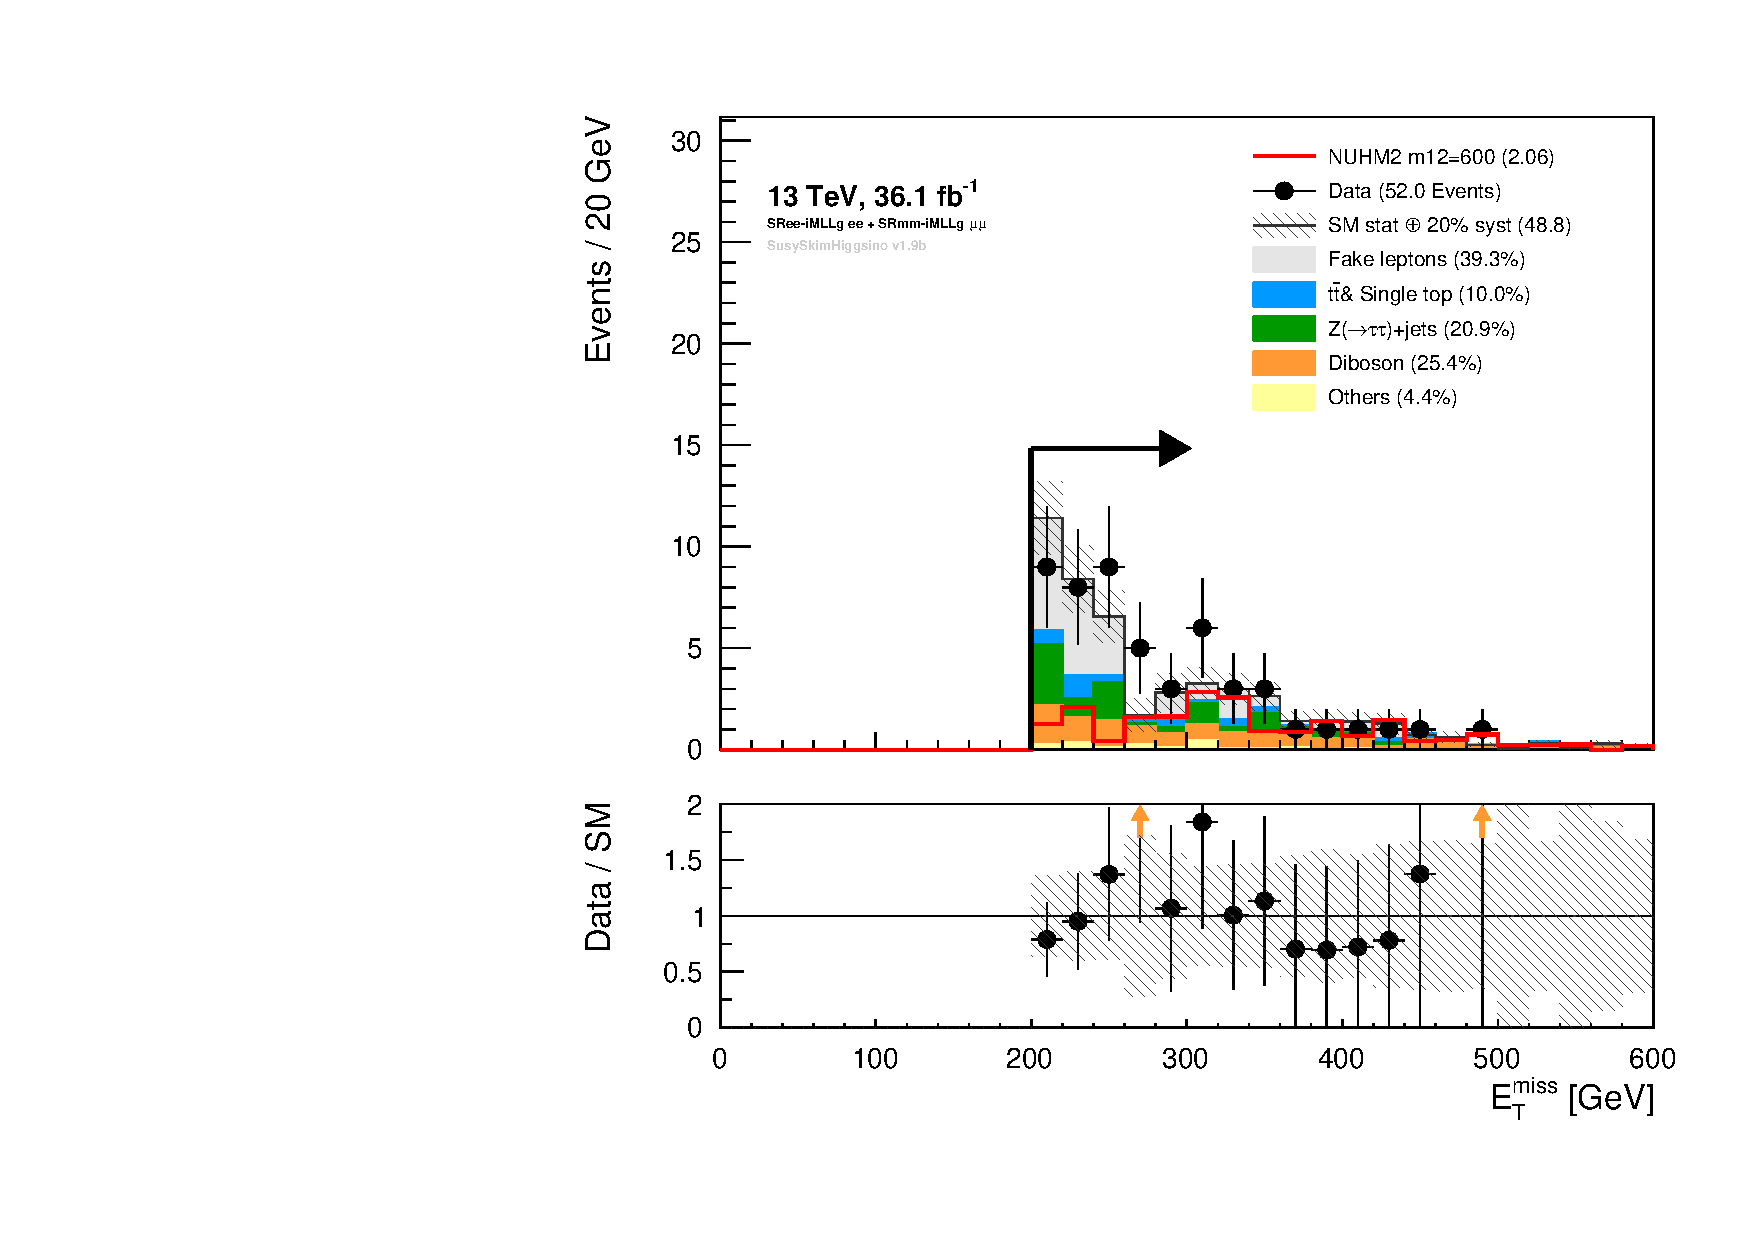
\includegraphics[scale=0.3]{NUHM2_m12_600_and_Bkg_met_Et_SFOS_N_minus_one_distribution_in_SR_times_10_on_Nsig.pdf}
            \caption{$E^{\mathrm{miss}}_{\mathrm{T}}$}
            \label{fig:event_nuhm2_m12_600_met_SFOS}
        \end{subfigure}
        \begin{subfigure}[b]{0.48\textwidth}
            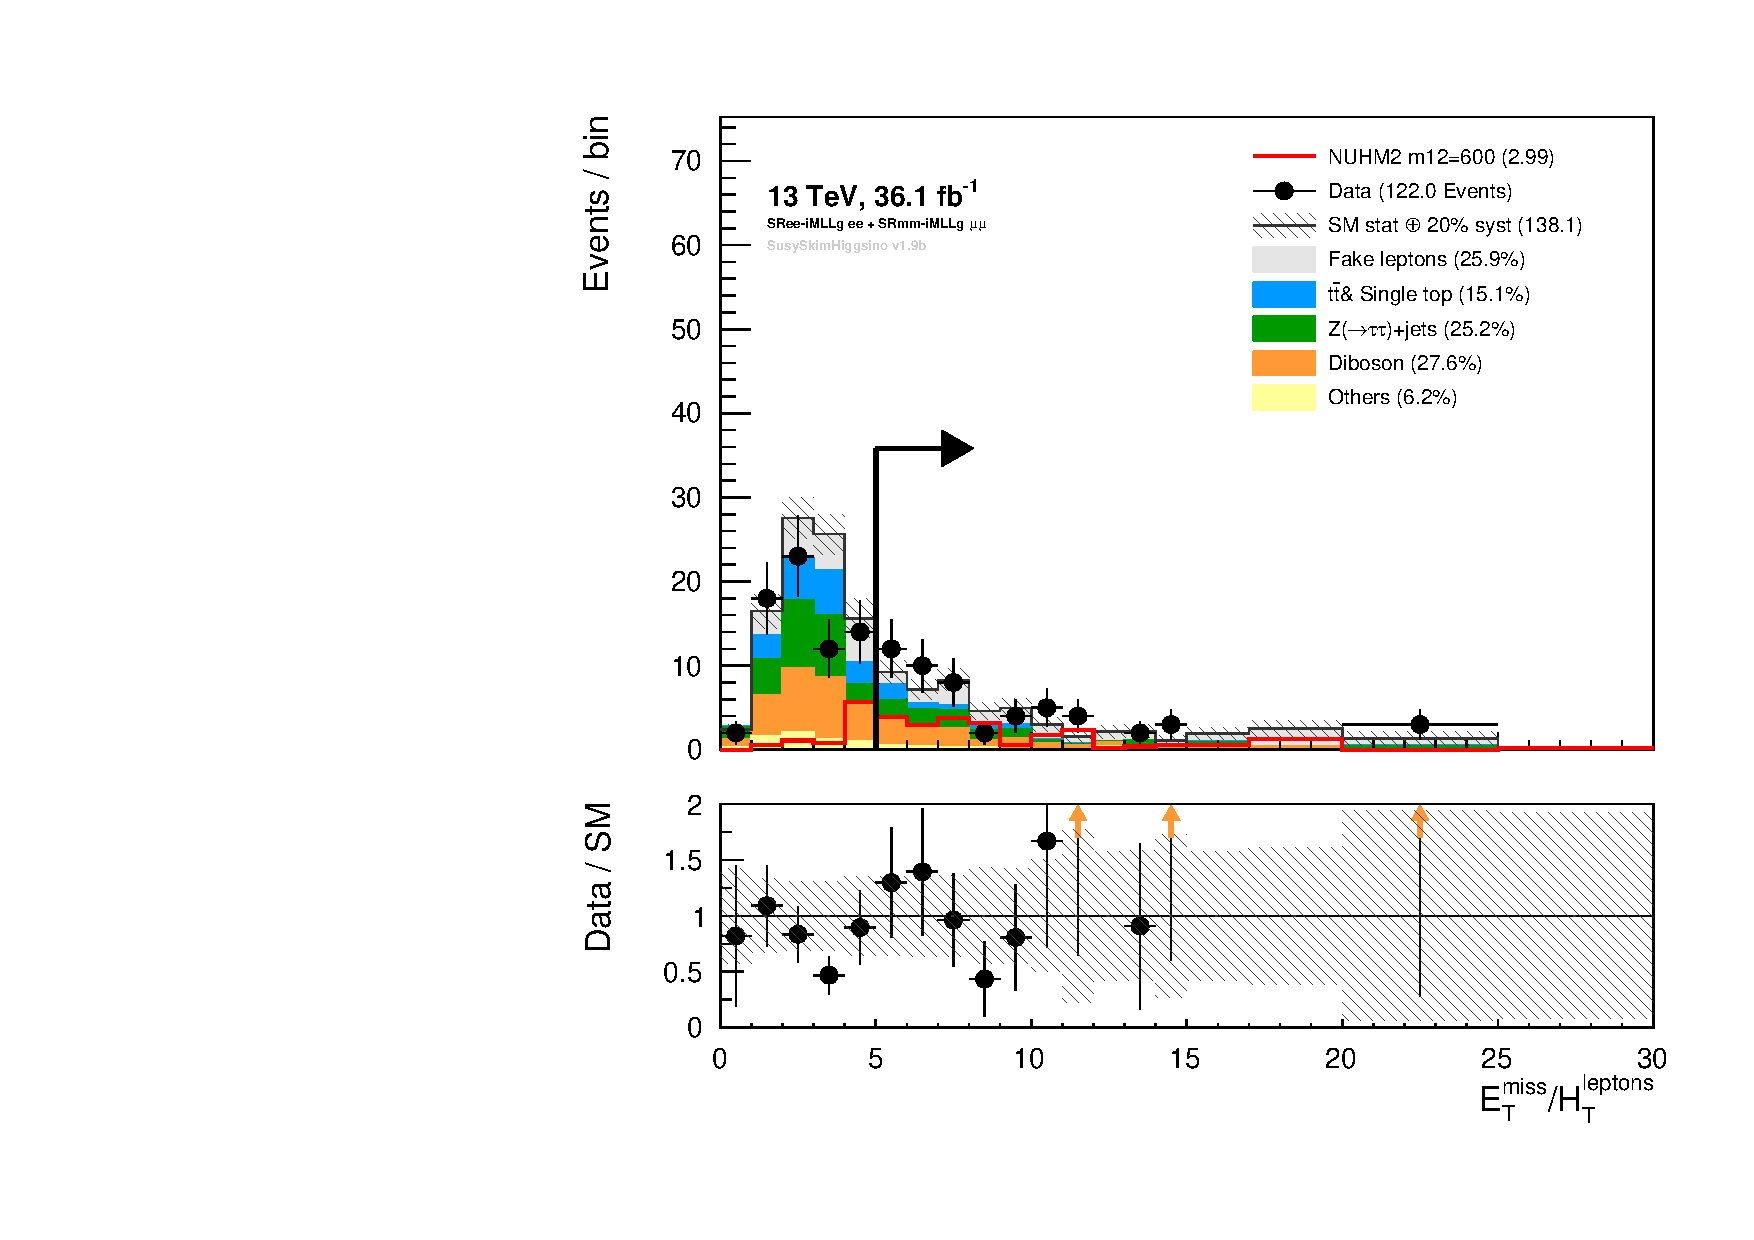
\includegraphics[scale=0.3]{NUHM2_m12_600_and_Bkg_METOverHTLep_SFOS_N_minus_one_distribution_in_SR_times_10_on_Nsig.pdf}
            \caption{$E^{\mathrm{miss}}_{\mathrm{T}} / H^{\mathrm{leptons}}_{\mathrm{T}}$}
            \label{fig:event_nuhm2_m12_600_METOverHTLep_SFOS}
        \end{subfigure}
    \end{center}
    \caption{The `$N-1$' distributions for NUHM2 model with $m_{1/2} = 600$~{\GeV} in SR region $1 < $SR$\ell \ell$-$m_{\ell \ell} < 60$~{\GeV}.
    The NUHM2 distributions are multiplied by 10 but the number of events in the legend use its actual values.}
    \label{fig:event_nuhm2_kinematic_in_SR_SFOS_m12_600_1}
\end{figure}

\begin{figure}[htbp]
    \begin{center}
        \begin{subfigure}[b]{0.48\textwidth}
            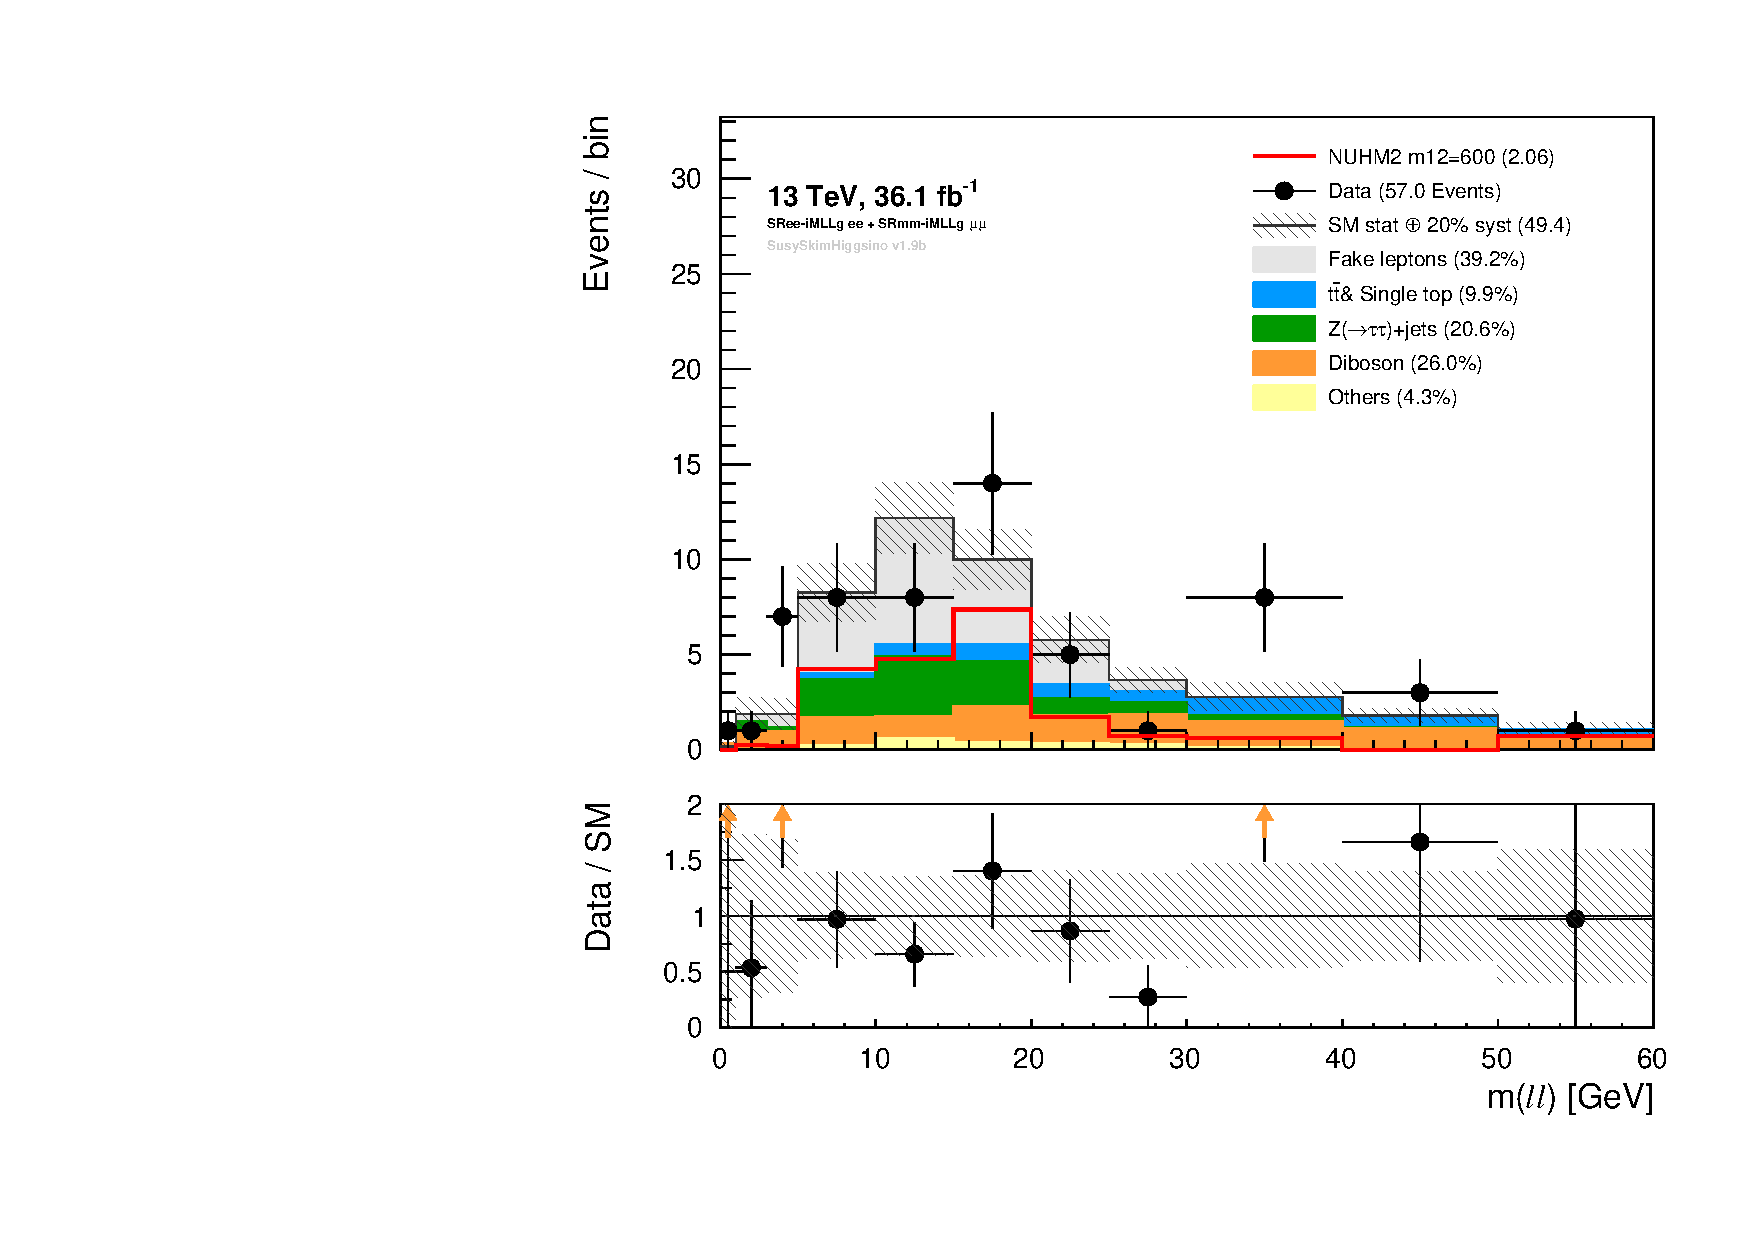
\includegraphics[scale=0.3]{NUHM2_m12_600_and_Bkg_mll_SFOS_N_minus_one_distribution_in_SR_times_10_on_Nsig.pdf}
            \caption{$m_{\ell\ell}$}
            \label{fig:event_nuhm2_m12_600_mll_SFOS}
        \end{subfigure}
        \begin{subfigure}[b]{0.48\textwidth}
            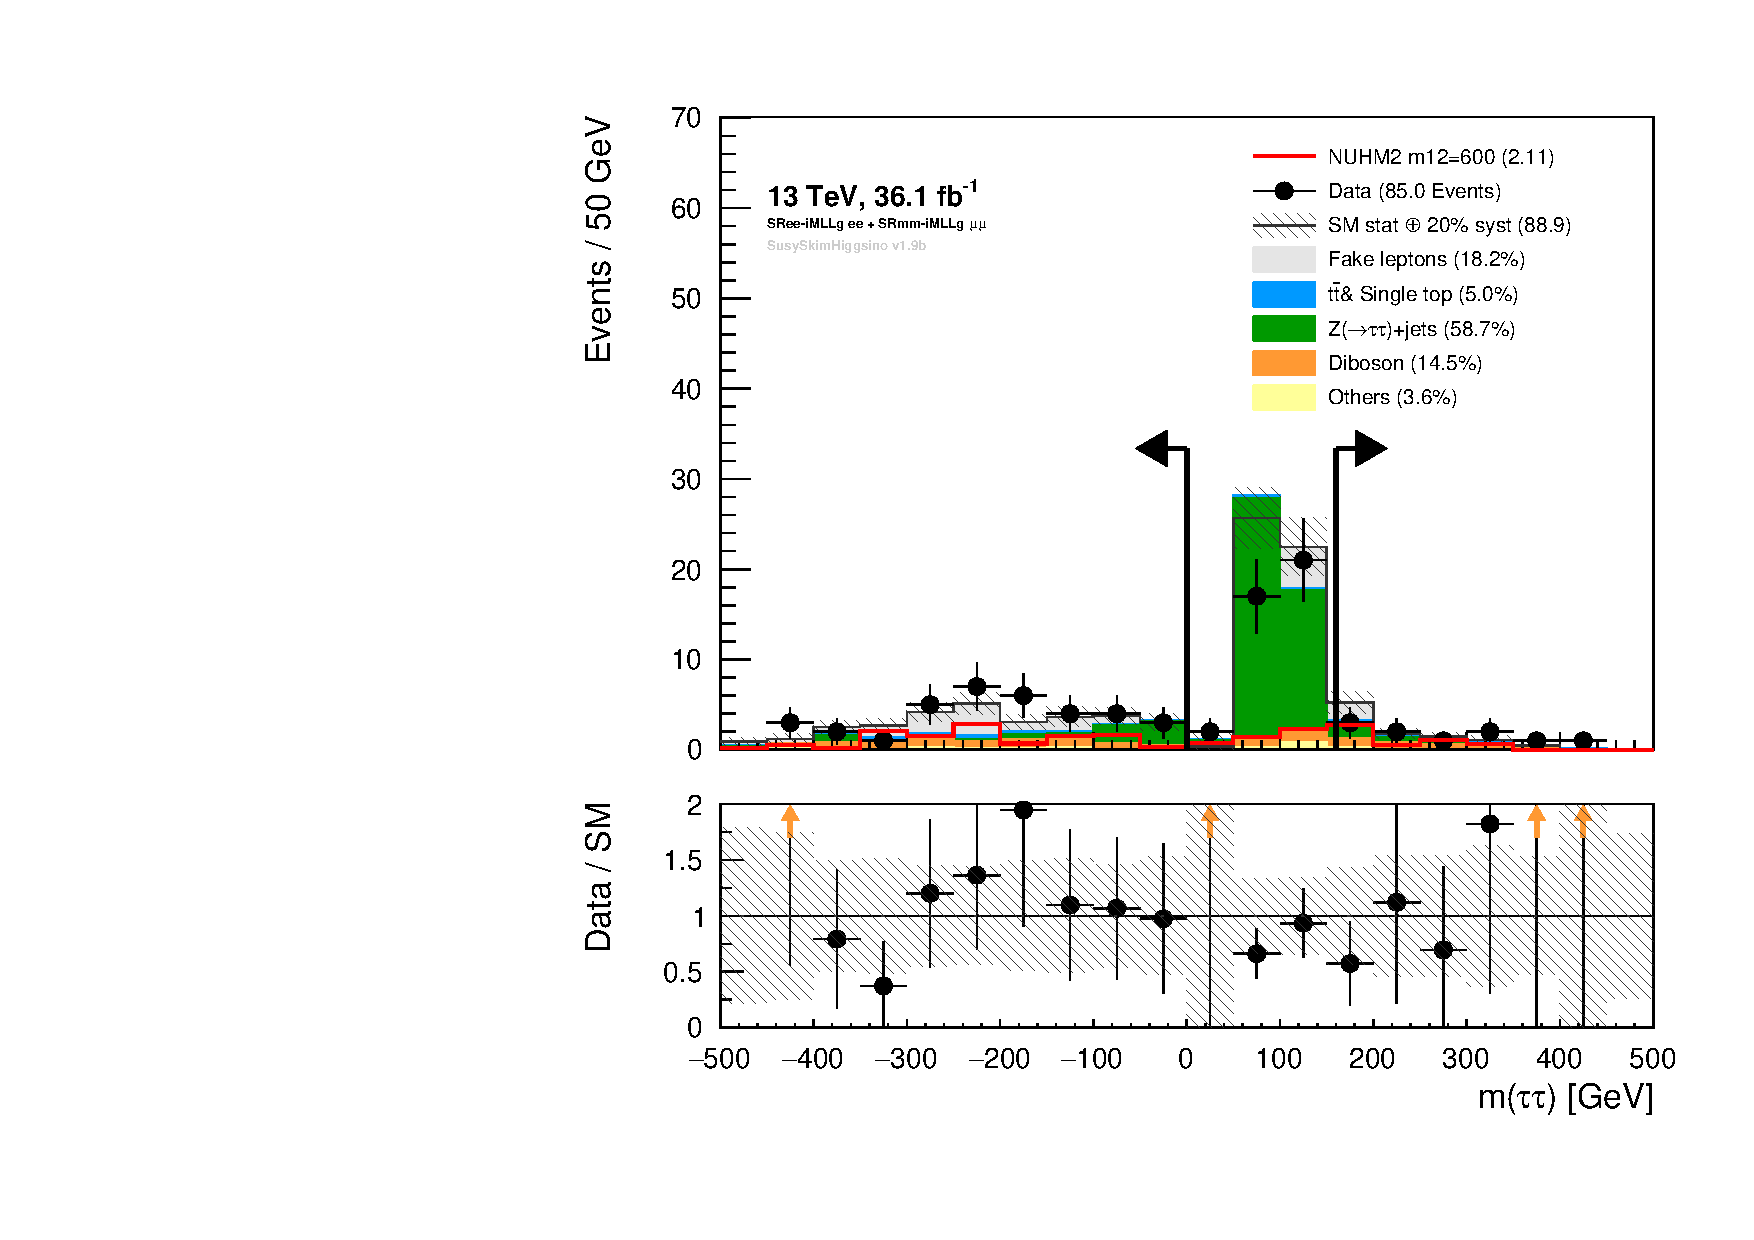
\includegraphics[scale=0.3]{NUHM2_m12_600_and_Bkg_MTauTau_SFOS_N_minus_one_distribution_in_SR_times_10_on_Nsig.pdf}
            \caption{$m_{\tau\tau}$}
            \label{fig:event_nuhm2_m12_600_MTauTau_SFOS}
        \end{subfigure}
        \begin{subfigure}[b]{0.48\textwidth}
            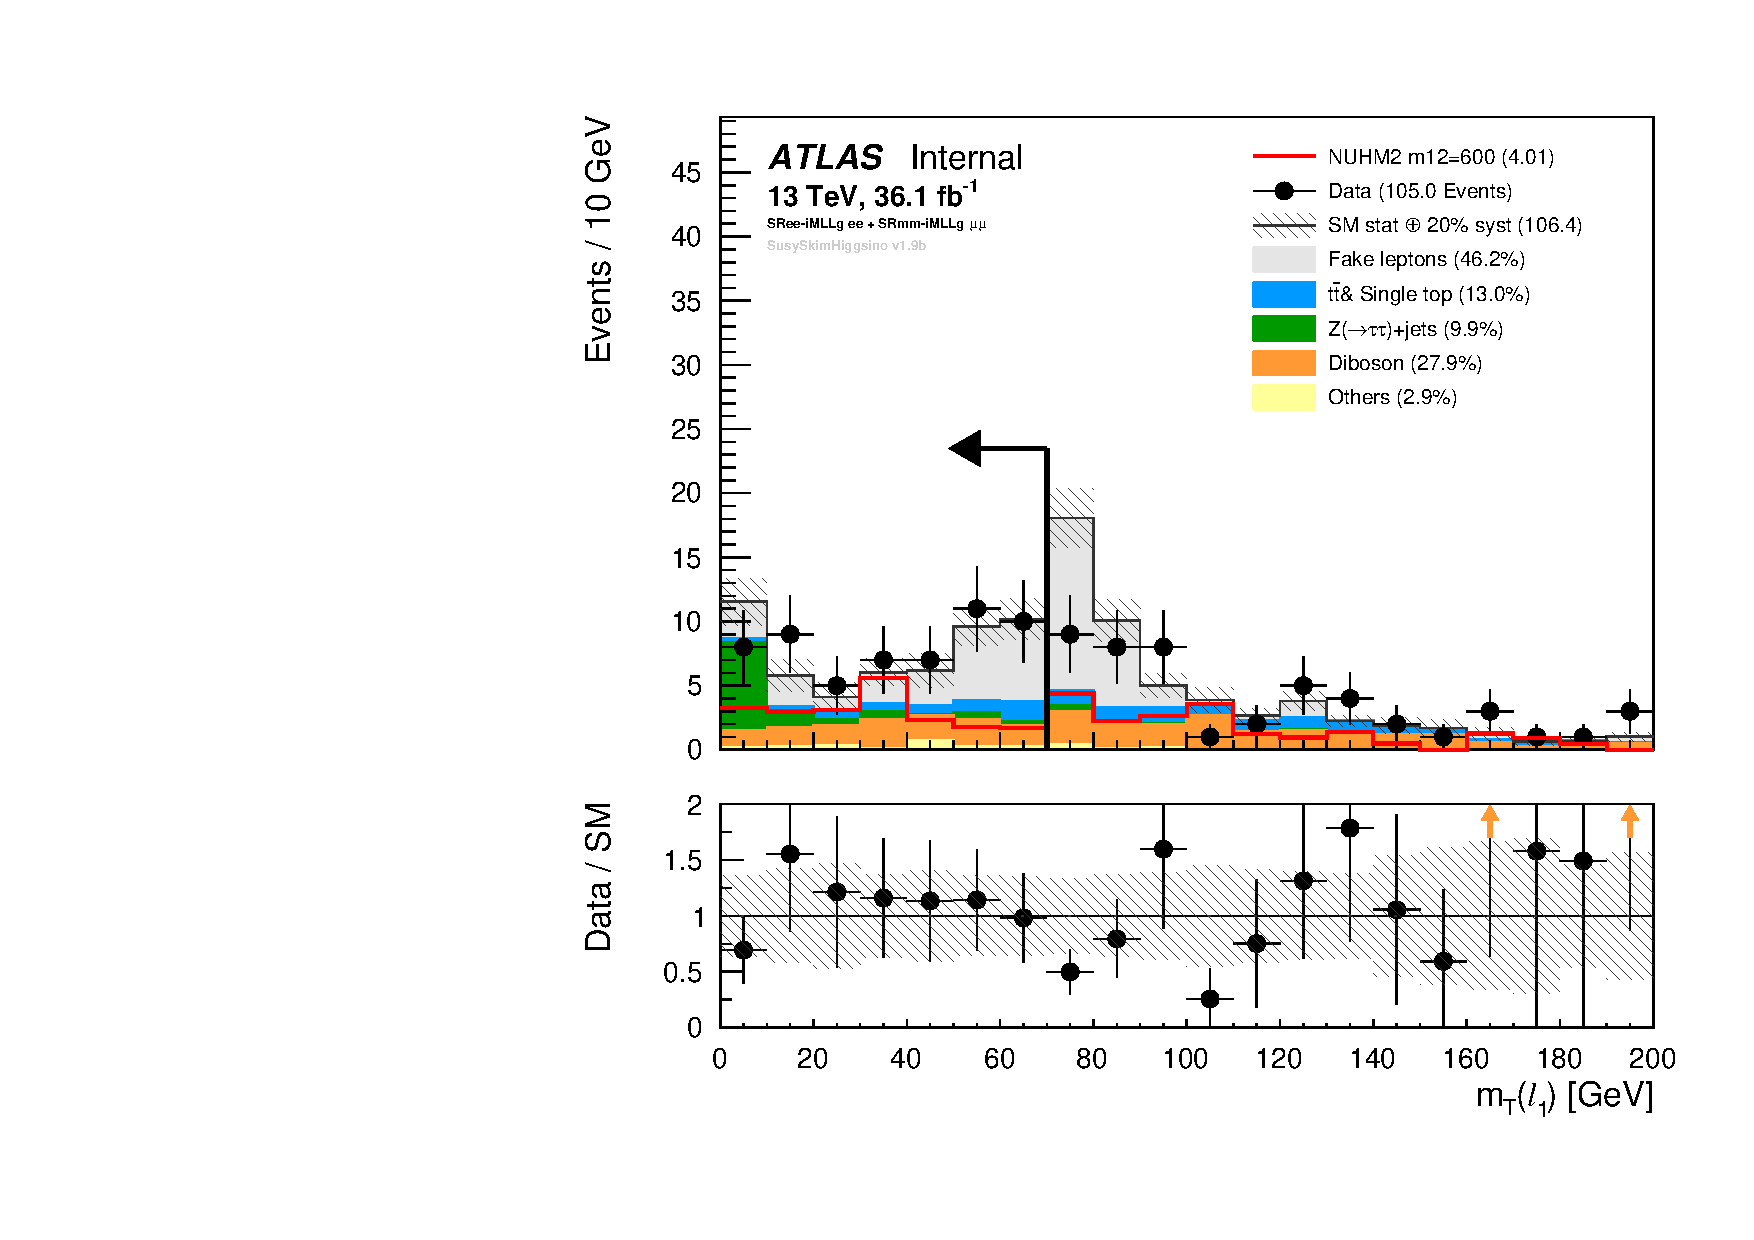
\includegraphics[scale=0.3]{NUHM2_m12_600_and_Bkg_mt_lep1_SFOS_N_minus_one_distribution_in_SR_times_10_on_Nsig.pdf}
            \caption{$m_{T}(\ell_{1})$}
            \label{fig:event_nuhm2_m12_600_mt_lep1_SFOS}
        \end{subfigure}
        \begin{subfigure}[b]{0.48\textwidth}
            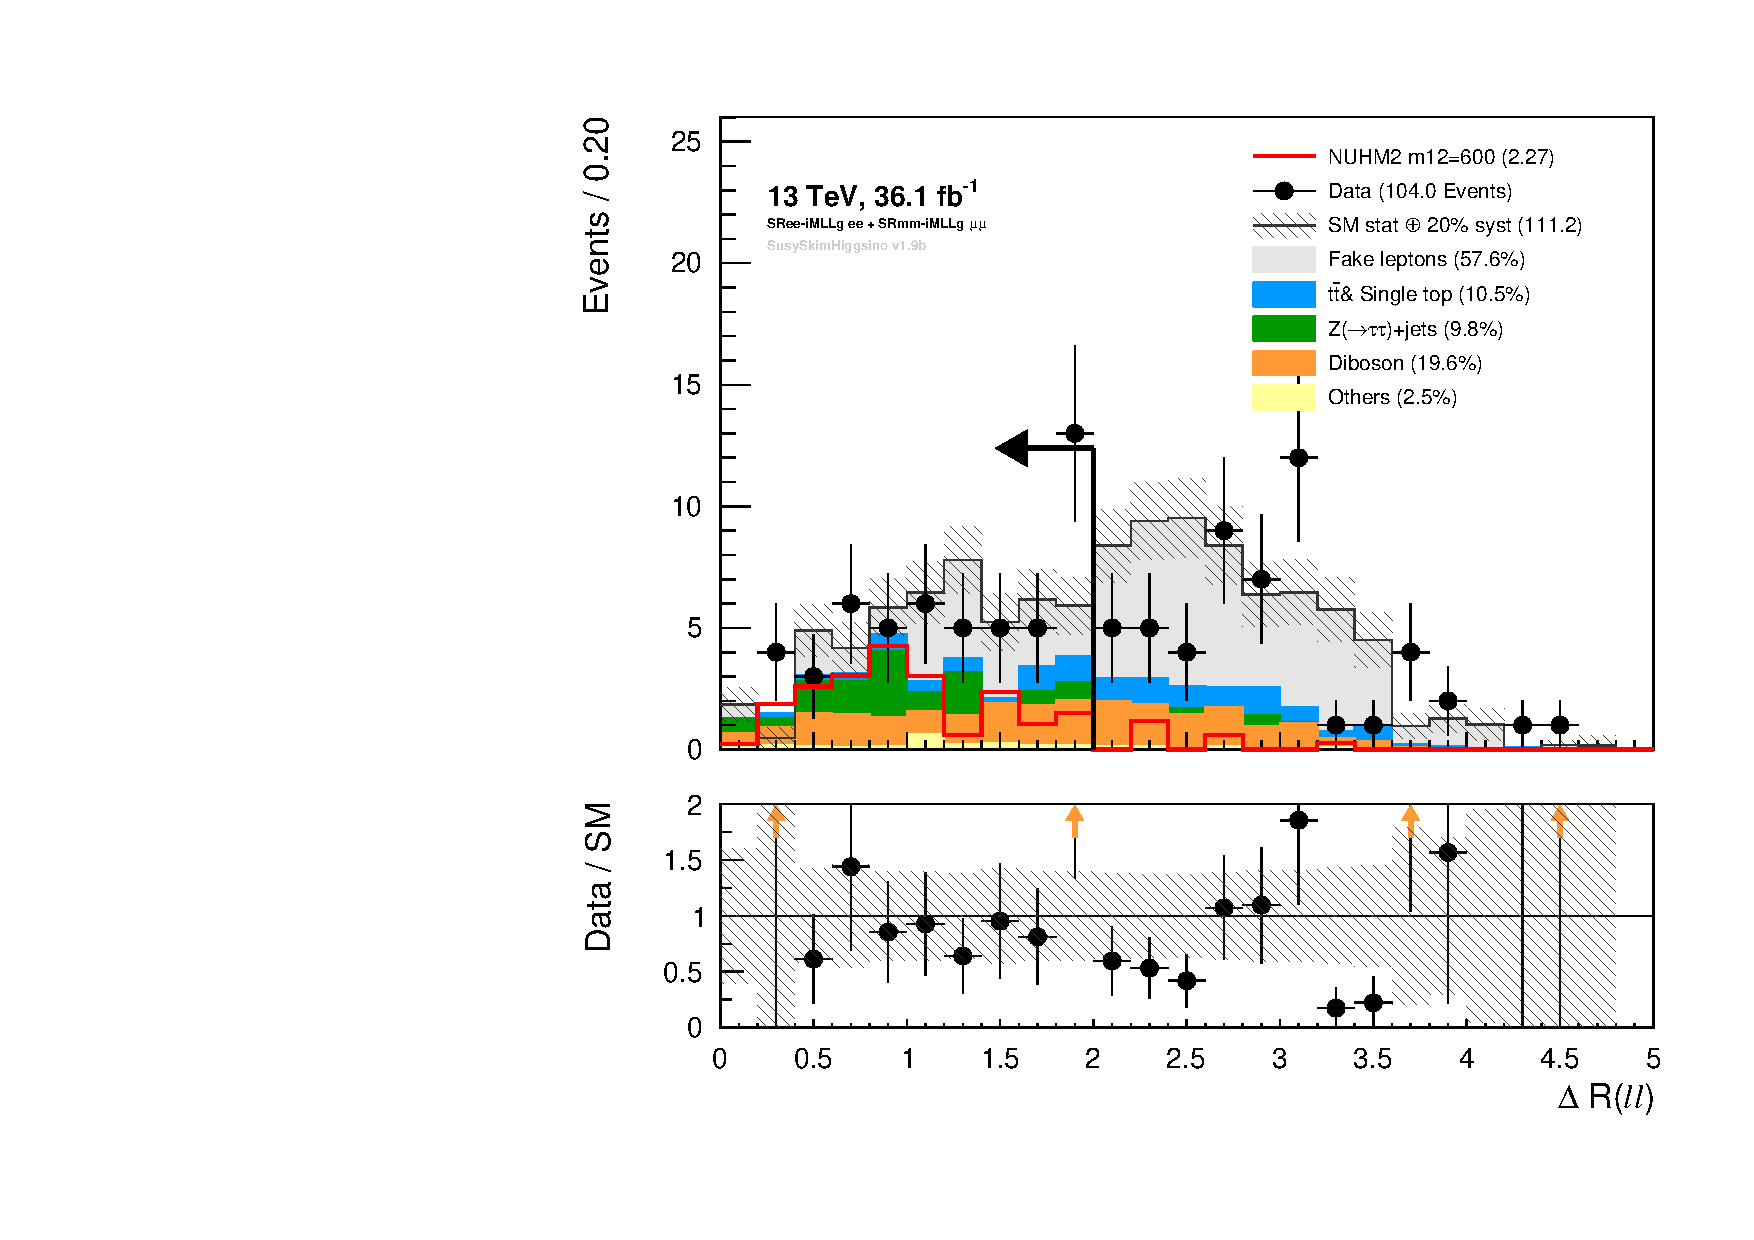
\includegraphics[scale=0.3]{NUHM2_m12_600_and_Bkg_Rll_SFOS_N_minus_one_distribution_in_SR_times_10_on_Nsig.pdf}
            \caption{$\Delta R_{\ell\ell}$}
            \label{fig:event_nuhm2_m12_600_Rll_SFOS}
        \end{subfigure}
        \begin{subfigure}[b]{0.48\textwidth}
            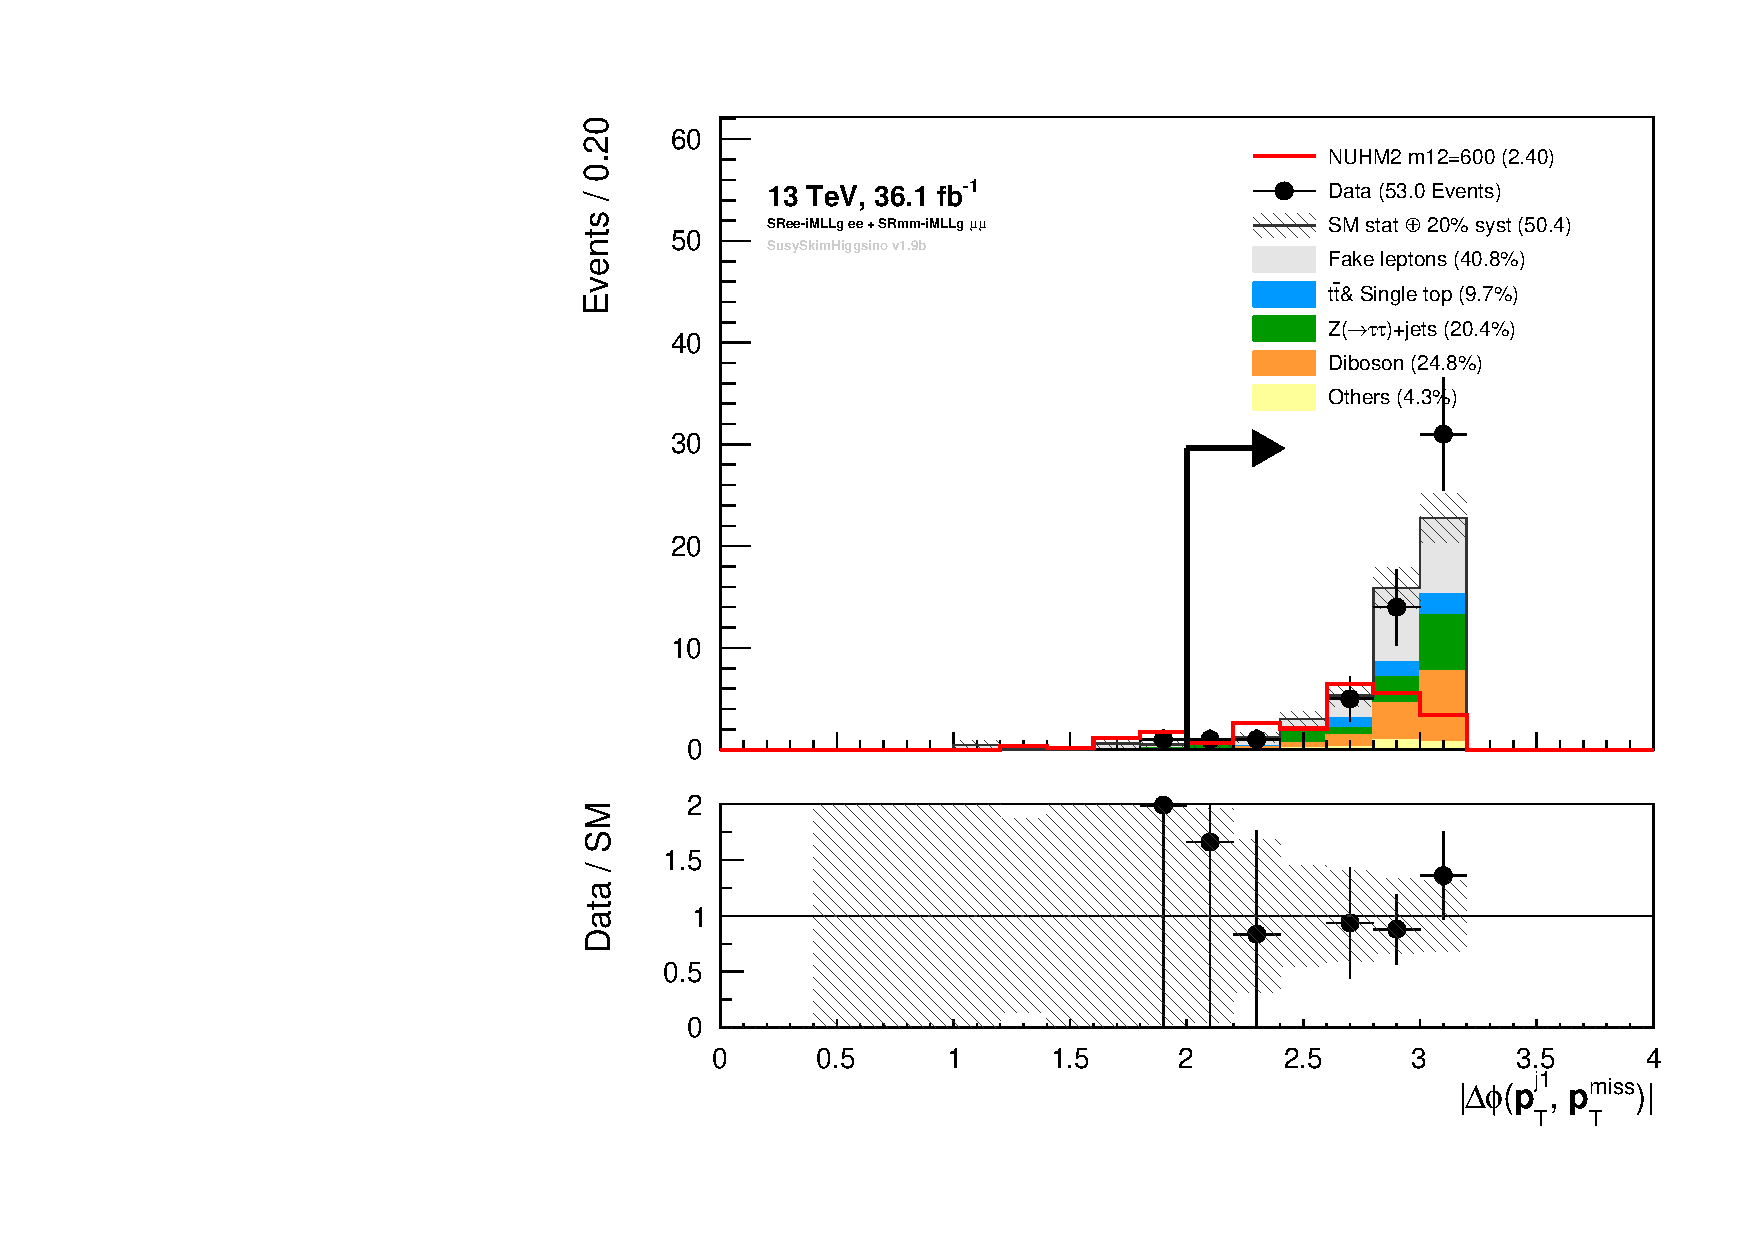
\includegraphics[scale=0.3]{NUHM2_m12_600_and_Bkg_DPhiJ1Met_SFOS_N_minus_one_distribution_in_SR_times_10_on_Nsig.pdf}
            \caption{$|\Delta \phi(\mathbf{p}^{j_{1}}_{\mathrm{T}}, \mathbf{p}^{\mathrm{miss}}_{\mathrm{T}})|$}
            \label{fig:event_nuhm2_m12_600_DPhiJ1Met_SFOS}
        \end{subfigure}
        \begin{subfigure}[b]{0.48\textwidth}
            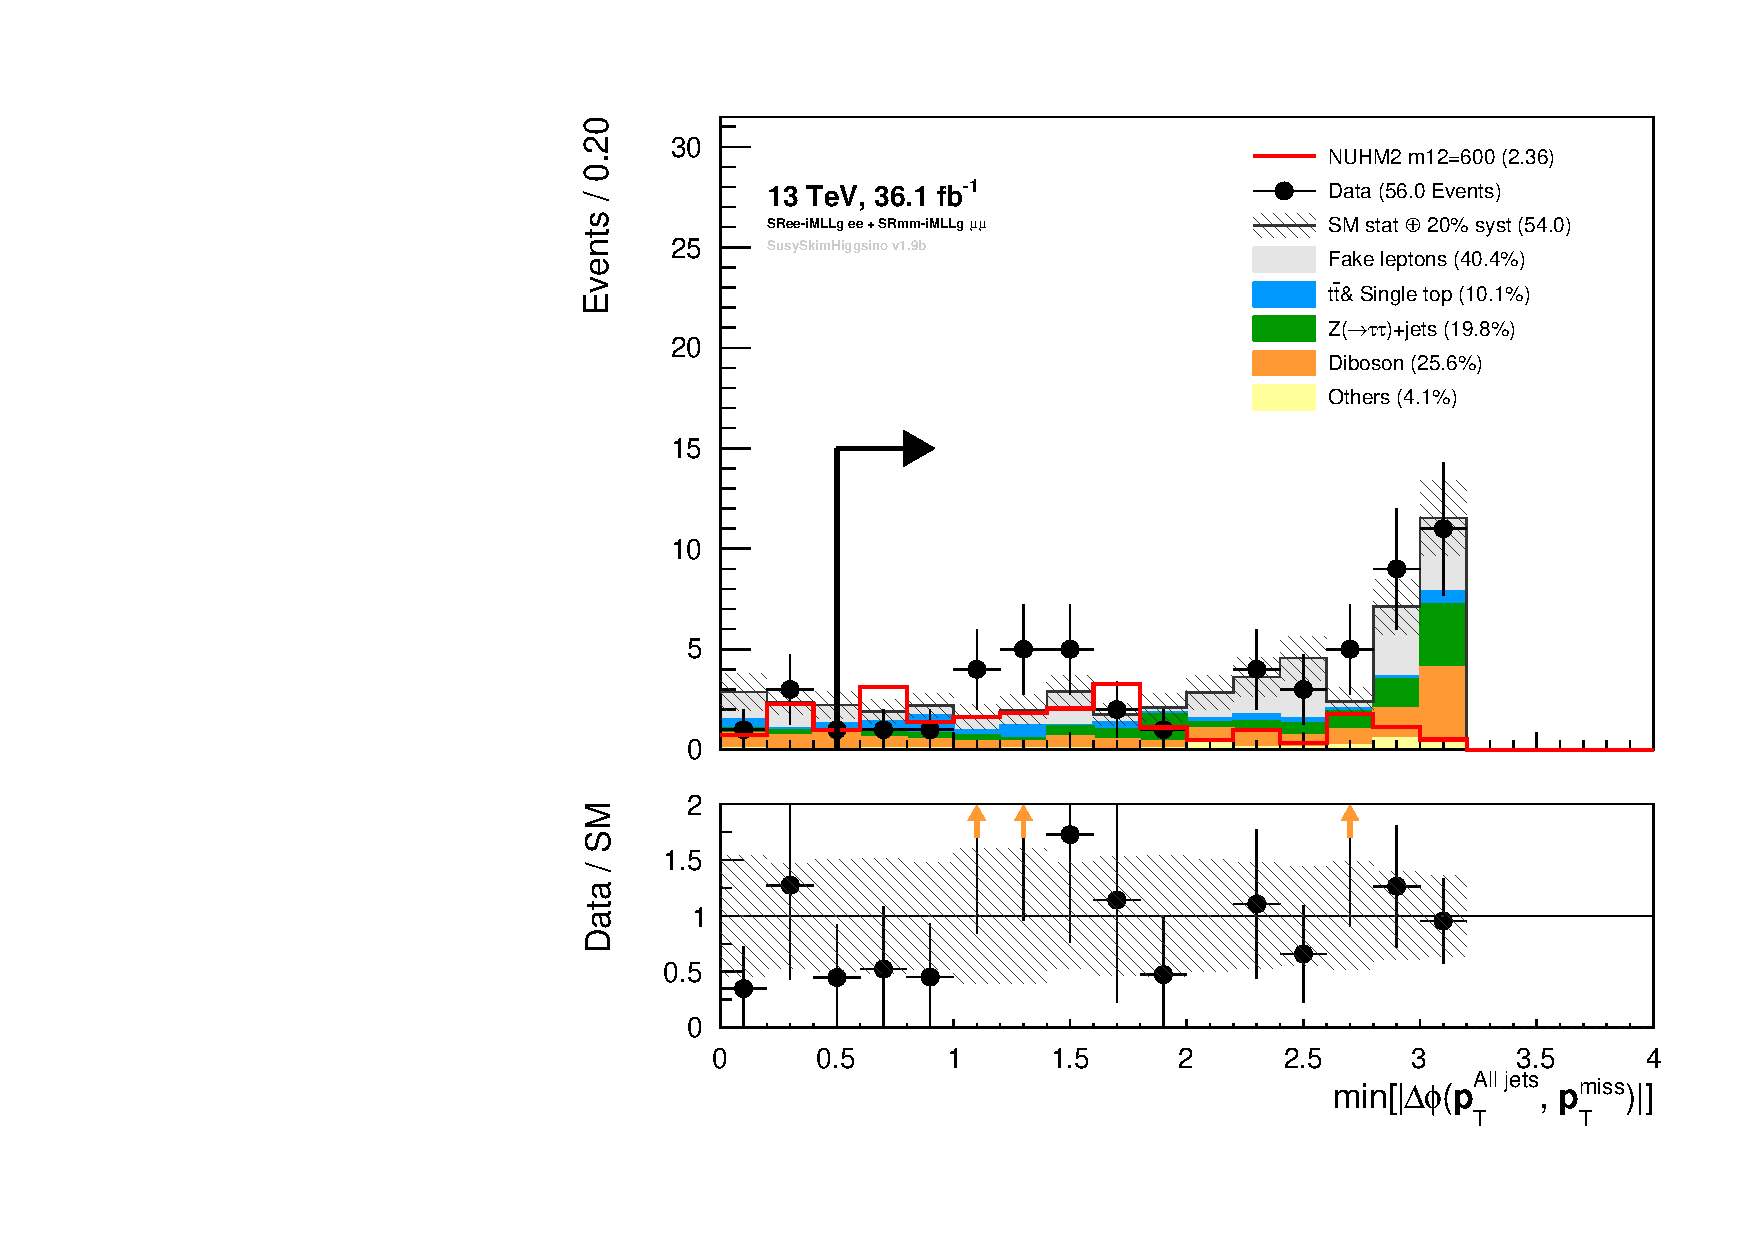
\includegraphics[scale=0.3]{NUHM2_m12_600_and_Bkg_minDPhiAllJetsMet_SFOS_N_minus_one_distribution_in_SR_times_10_on_Nsig.pdf}
            \caption{min[$|\Delta \phi(\mathbf{p}^{\textrm{All jets}}_{\mathrm{T}}, \mathbf{p}^{\mathrm{miss}}_{\mathrm{T}})|$]}
            \label{fig:event_nuhm2_m12_600_minDPhiAllJetsMet_SFOS}
        \end{subfigure}
    \end{center}
    \caption{The `$N-1$' distributions for NUHM2 model with $m_{1/2} = 600$~{\GeV} in SR region $1 < $SR$\ell \ell$-$m_{\ell \ell} < 60$~{\GeV}.
    The NUHM2 distributions are multiplied by 10 but the number of events in the legend use its actual values.}
    \label{fig:event_nuhm2_kinematic_in_SR_SFOS_m12_600_2}
\end{figure}

% m12 = 700
\begin{figure}[htbp]
    \begin{center}
        \begin{subfigure}[b]{0.48\textwidth}
            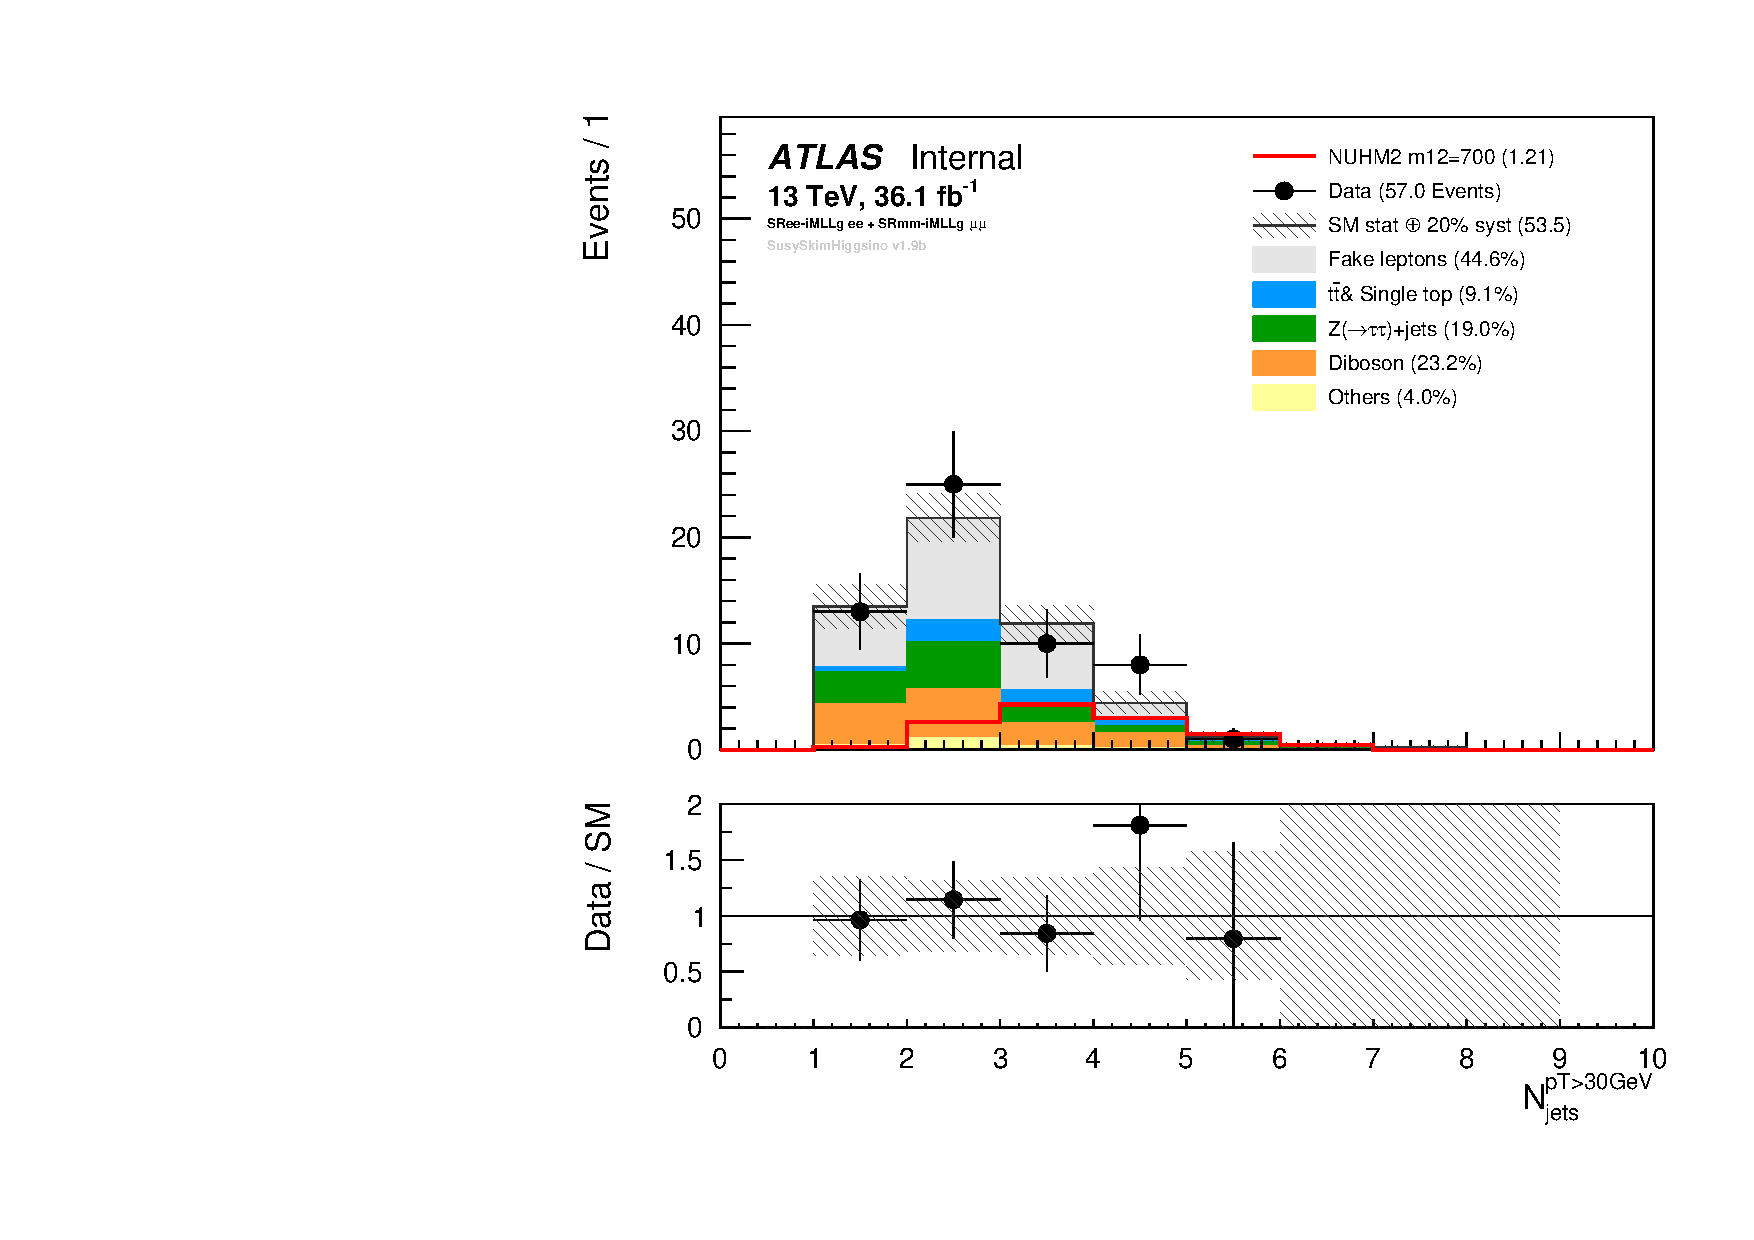
\includegraphics[scale=0.3]{NUHM2_m12_700_and_Bkg_nJet30_SFOS_N_minus_one_distribution_in_SR_times_10_on_Nsig.pdf}
            \caption{$N^{30}_{\mathrm{jets}}$}
            \label{fig:event_nuhm2_m12_700_nJet30_SFOS}
        \end{subfigure}
        \begin{subfigure}[b]{0.48\textwidth}
            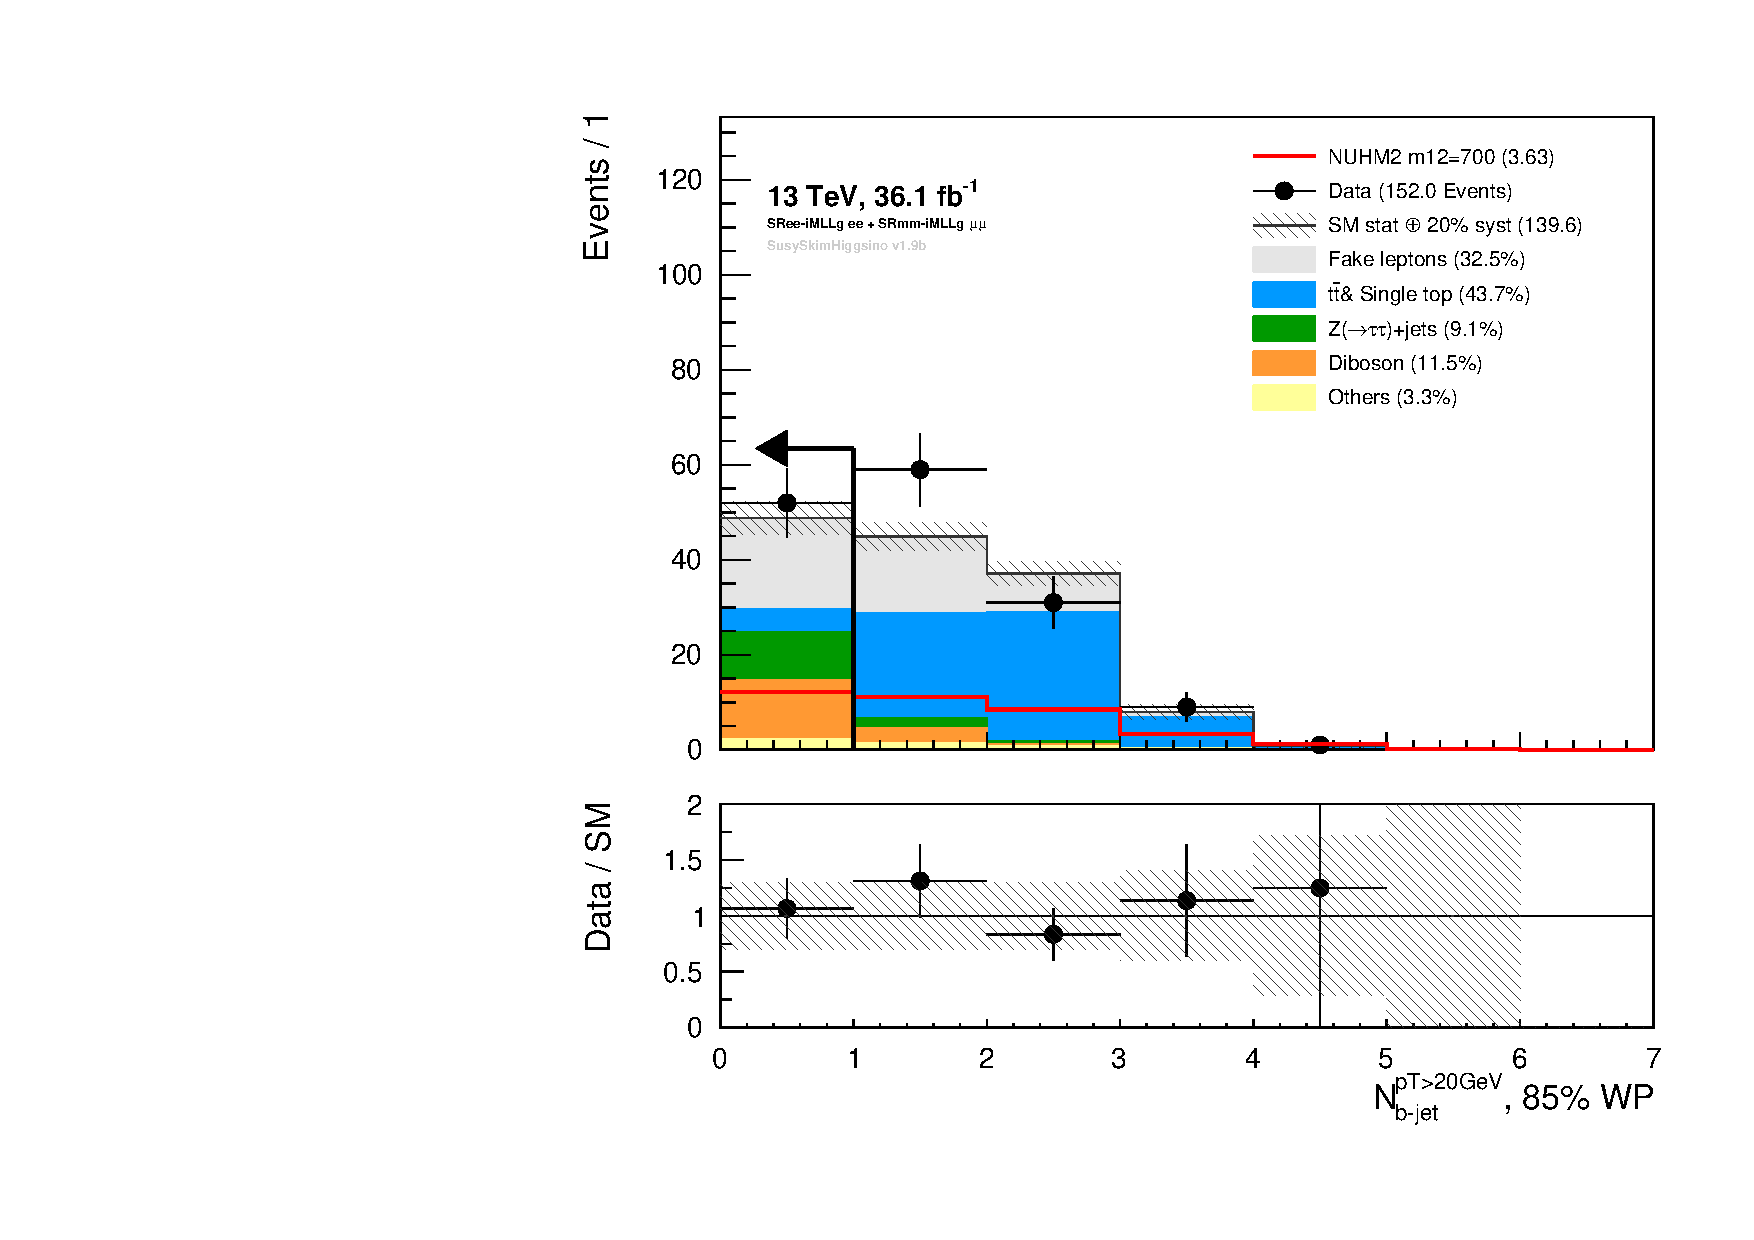
\includegraphics[scale=0.3]{NUHM2_m12_700_and_Bkg_nBJet20_MV2c10_SFOS_N_minus_one_distribution_in_SR_times_10_on_Nsig.pdf}
            \caption{$N^{20}_{\mathrm{b-jets}}$}
            \label{fig:event_nuhm2_m12_700_nBJet20_SFOS}
        \end{subfigure}
        \begin{subfigure}[b]{0.48\textwidth}
            \includegraphics[scale=0.3]{NUHM2_m12_700_and_Bkg_lep1Pt_SFOS_N_minus_one_distribution_in_SR_times_10_on_Nsig.pdf}
            \caption{$p^{\ell_1}_{\mathrm{T}}$}
            \label{fig:event_nuhm2_m12_700_lep1Pt_SFOS}
        \end{subfigure}
        \begin{subfigure}[b]{0.48\textwidth}
            \includegraphics[scale=0.3]{NUHM2_m12_700_and_Bkg_lep2Pt_SFOS_N_minus_one_distribution_in_SR_times_10_on_Nsig.pdf}
            \caption{$p^{\ell_2}_{\mathrm{T}}$}
            \label{fig:event_nuhm2_m12_700_lep2Pt_SFOS}
        \end{subfigure}
        \begin{subfigure}[b]{0.48\textwidth}
            \includegraphics[scale=0.3]{NUHM2_m12_700_and_Bkg_met_Et_SFOS_N_minus_one_distribution_in_SR_times_10_on_Nsig.pdf}
            \caption{$E^{\mathrm{miss}}_{\mathrm{T}}$}
            \label{fig:event_nuhm2_m12_700_met_SFOS}
        \end{subfigure}
        \begin{subfigure}[b]{0.48\textwidth}
            \includegraphics[scale=0.3]{NUHM2_m12_700_and_Bkg_METOverHTLep_SFOS_N_minus_one_distribution_in_SR_times_10_on_Nsig.pdf}
            \caption{$E^{\mathrm{miss}}_{\mathrm{T}} / H^{\mathrm{leptons}}_{\mathrm{T}}$}
            \label{fig:event_nuhm2_m12_700_METOverHTLep_SFOS}
        \end{subfigure}
    \end{center}
    \caption{The `$N-1$' distributions for NUHM2 model with $m_{1/2} = 700$~{\GeV} in SR region $1 < $SR$\ell \ell$-$m_{\ell \ell} < 60$~{\GeV}.
    The NUHM2 distributions are multiplied by 10 but the number of events in the legend use its actual values.}
    \label{fig:event_nuhm2_kinematic_in_SR_SFOS_m12_700_1}
\end{figure}

\begin{figure}[htbp]
    \begin{center}
        \begin{subfigure}[b]{0.48\textwidth}
            \includegraphics[scale=0.3]{NUHM2_m12_700_and_Bkg_mll_SFOS_N_minus_one_distribution_in_SR_times_10_on_Nsig.pdf}
            \caption{$m_{\ell\ell}$}
            \label{fig:event_nuhm2_m12_700_mll_SFOS}
        \end{subfigure}
        \begin{subfigure}[b]{0.48\textwidth}
            \includegraphics[scale=0.3]{NUHM2_m12_700_and_Bkg_MTauTau_SFOS_N_minus_one_distribution_in_SR_times_10_on_Nsig.pdf}
            \caption{$m_{\tau\tau}$}
            \label{fig:event_nuhm2_m12_700_MTauTau_SFOS}
        \end{subfigure}
        \begin{subfigure}[b]{0.48\textwidth}
            \includegraphics[scale=0.3]{NUHM2_m12_700_and_Bkg_mt_lep1_SFOS_N_minus_one_distribution_in_SR_times_10_on_Nsig.pdf}
            \caption{$m_{T}(\ell_{1})$}
            \label{fig:event_nuhm2_m12_700_mt_lep1_SFOS}
        \end{subfigure}
        \begin{subfigure}[b]{0.48\textwidth}
            \includegraphics[scale=0.3]{NUHM2_m12_700_and_Bkg_Rll_SFOS_N_minus_one_distribution_in_SR_times_10_on_Nsig.pdf}
            \caption{$\Delta R_{\ell\ell}$}
            \label{fig:event_nuhm2_m12_700_Rll_SFOS}
        \end{subfigure}
        \begin{subfigure}[b]{0.48\textwidth}
            \includegraphics[scale=0.3]{NUHM2_m12_700_and_Bkg_DPhiJ1Met_SFOS_N_minus_one_distribution_in_SR_times_10_on_Nsig.pdf}
            \caption{$|\Delta \phi(\mathbf{p}^{j_{1}}_{\mathrm{T}}, \mathbf{p}^{\mathrm{miss}}_{\mathrm{T}})|$}
            \label{fig:event_nuhm2_m12_700_DPhiJ1Met_SFOS}
        \end{subfigure}
        \begin{subfigure}[b]{0.48\textwidth}
            \includegraphics[scale=0.3]{NUHM2_m12_700_and_Bkg_minDPhiAllJetsMet_SFOS_N_minus_one_distribution_in_SR_times_10_on_Nsig.pdf}
            \caption{min[$|\Delta \phi(\mathbf{p}^{\textrm{All jets}}_{\mathrm{T}}, \mathbf{p}^{\mathrm{miss}}_{\mathrm{T}})|$]}
            \label{fig:event_nuhm2_m12_700_minDPhiAllJetsMet_SFOS}
        \end{subfigure}
    \end{center}
    \caption{The `$N-1$' distributions for NUHM2 model with $m_{1/2} = 700$~{\GeV} in SR region $1 < $SR$\ell \ell$-$m_{\ell \ell} < 60$~{\GeV}.
    The NUHM2 distributions are multiplied by 10 but the number of events in the legend use its actual values.}
    \label{fig:event_nuhm2_kinematic_in_SR_SFOS_m12_700_2}
\end{figure}

% m12 = 800
\begin{figure}[htbp]
    \begin{center}
        \begin{subfigure}[b]{0.48\textwidth}
            \includegraphics[scale=0.3]{NUHM2_m12_800_and_Bkg_nJet30_SFOS_N_minus_one_distribution_in_SR_times_10_on_Nsig.pdf}
            \caption{$N^{30}_{\mathrm{jets}}$}
            \label{fig:event_nuhm2_m12_800_nJet30_SFOS}
        \end{subfigure}
        \begin{subfigure}[b]{0.48\textwidth}
            \includegraphics[scale=0.3]{NUHM2_m12_800_and_Bkg_nBJet20_MV2c10_SFOS_N_minus_one_distribution_in_SR_times_10_on_Nsig.pdf}
            \caption{$N^{20}_{\mathrm{b-jets}}$}
            \label{fig:event_nuhm2_m12_800_nBJet20_SFOS}
        \end{subfigure}
        \begin{subfigure}[b]{0.48\textwidth}
            \includegraphics[scale=0.3]{NUHM2_m12_800_and_Bkg_lep1Pt_SFOS_N_minus_one_distribution_in_SR_times_10_on_Nsig.pdf}
            \caption{$p^{\ell_1}_{\mathrm{T}}$}
            \label{fig:event_nuhm2_m12_800_lep1Pt_SFOS}
        \end{subfigure}
        \begin{subfigure}[b]{0.48\textwidth}
            \includegraphics[scale=0.3]{NUHM2_m12_800_and_Bkg_lep2Pt_SFOS_N_minus_one_distribution_in_SR_times_10_on_Nsig.pdf}
            \caption{$p^{\ell_2}_{\mathrm{T}}$}
            \label{fig:event_nuhm2_m12_800_lep2Pt_SFOS}
        \end{subfigure}
        \begin{subfigure}[b]{0.48\textwidth}
            \includegraphics[scale=0.3]{NUHM2_m12_800_and_Bkg_met_Et_SFOS_N_minus_one_distribution_in_SR_times_10_on_Nsig.pdf}
            \caption{$E^{\mathrm{miss}}_{\mathrm{T}}$}
            \label{fig:event_nuhm2_m12_800_met_SFOS}
        \end{subfigure}
        \begin{subfigure}[b]{0.48\textwidth}
            \includegraphics[scale=0.3]{NUHM2_m12_800_and_Bkg_METOverHTLep_SFOS_N_minus_one_distribution_in_SR_times_10_on_Nsig.pdf}
            \caption{$E^{\mathrm{miss}}_{\mathrm{T}} / H^{\mathrm{leptons}}_{\mathrm{T}}$}
            \label{fig:event_nuhm2_m12_800_METOverHTLep_SFOS}
        \end{subfigure}
    \end{center}
    \caption{The `$N-1$' distributions for NUHM2 model with $m_{1/2} = 800$~{\GeV} in SR region $1 < $SR$\ell \ell$-$m_{\ell \ell} < 60$~{\GeV}.
    The NUHM2 distributions are multiplied by 10 but the number of events in the legend use its actual values.}
    \label{fig:event_nuhm2_kinematic_in_SR_SFOS_m12_800_1}
\end{figure}

\begin{figure}[htbp]
    \begin{center}
        \begin{subfigure}[b]{0.48\textwidth}
            \includegraphics[scale=0.3]{NUHM2_m12_800_and_Bkg_mll_SFOS_N_minus_one_distribution_in_SR_times_10_on_Nsig.pdf}
            \caption{$m_{\ell\ell}$}
            \label{fig:event_nuhm2_m12_800_mll_SFOS}
        \end{subfigure}
        \begin{subfigure}[b]{0.48\textwidth}
            \includegraphics[scale=0.3]{NUHM2_m12_800_and_Bkg_MTauTau_SFOS_N_minus_one_distribution_in_SR_times_10_on_Nsig.pdf}
            \caption{$m_{\tau\tau}$}
            \label{fig:event_nuhm2_m12_800_MTauTau_SFOS}
        \end{subfigure}
        \begin{subfigure}[b]{0.48\textwidth}
            \includegraphics[scale=0.3]{NUHM2_m12_800_and_Bkg_mt_lep1_SFOS_N_minus_one_distribution_in_SR_times_10_on_Nsig.pdf}
            \caption{$m_{T}(\ell_{1})$}
            \label{fig:event_nuhm2_m12_800_mt_lep1_SFOS}
        \end{subfigure}
        \begin{subfigure}[b]{0.48\textwidth}
            \includegraphics[scale=0.3]{NUHM2_m12_800_and_Bkg_Rll_SFOS_N_minus_one_distribution_in_SR_times_10_on_Nsig.pdf}
            \caption{$\Delta R_{\ell\ell}$}
            \label{fig:event_nuhm2_m12_800_Rll_SFOS}
        \end{subfigure}
        \begin{subfigure}[b]{0.48\textwidth}
            \includegraphics[scale=0.3]{NUHM2_m12_800_and_Bkg_DPhiJ1Met_SFOS_N_minus_one_distribution_in_SR_times_10_on_Nsig.pdf}
            \caption{$|\Delta \phi(\mathbf{p}^{j_{1}}_{\mathrm{T}}, \mathbf{p}^{\mathrm{miss}}_{\mathrm{T}})|$}
            \label{fig:event_nuhm2_m12_800_DPhiJ1Met_SFOS}
        \end{subfigure}
        \begin{subfigure}[b]{0.48\textwidth}
            \includegraphics[scale=0.3]{NUHM2_m12_800_and_Bkg_minDPhiAllJetsMet_SFOS_N_minus_one_distribution_in_SR_times_10_on_Nsig.pdf}
            \caption{min[$|\Delta \phi(\mathbf{p}^{\textrm{All jets}}_{\mathrm{T}}, \mathbf{p}^{\mathrm{miss}}_{\mathrm{T}})|$]}
            \label{fig:event_nuhm2_m12_800_minDPhiAllJetsMet_SFOS}
        \end{subfigure}
    \end{center}
    \caption{The `$N-1$' distributions for NUHM2 model with $m_{1/2} = 800$~{\GeV} in SR region $1 < $SR$\ell \ell$-$m_{\ell \ell} < 60$~{\GeV}.
    The NUHM2 distributions are multiplied by 10 but the number of events in the legend use its actual values.}
    \label{fig:event_nuhm2_kinematic_in_SR_SFOS_m12_800_2}
\end{figure}